\documentclass[12pt,a4paper,figuresright]{book}

% make sure sessions and talks are not split between pages
\usepackage{needspace}
\usepackage[colorlinks=true,
linkcolor=blue,      % color of internal links
citecolor=green,     % color of citations
urlcolor=red         % color of URLs
]{hyperref}
%\usepackage{hyperref}
\usepackage{bm}
\usepackage{verbatim}
\usepackage{tabularx}
\usepackage{amsmath}
\usepackage{amssymb}
\usepackage{mathrsfs}

\usepackage{mcm_macros}

% Put date and time stamp, page number in footer
\usepackage{datetime}
\usepackage{fancyhdr}
\fancyhf{}
\fancyfoot[L]{\twodigit{\day}/\twodigit{\month}/\the\year\ \currenttime}
\fancyfoot[R]{\thepage}
\pagestyle{fancy}
\renewcommand{\headrulewidth}{0pt}
\renewcommand{\footrulewidth}{0.4pt}
\renewcommand{\dateseparator}{/}

% ------------------------------------------------------------------------
% Document begins here
% ------------------------------------------------------------------------
\begin{document}

% ------------------------------------------------------------------------
% ------------------------------------------------------------------------
% ------------------------------------------------------------------------
\chapter{The Fifteenth International Conference on Monte Carlo and Applications  (MCM 2025) }



% ------------------------------------------------------------------------
\section{Welcome}

We are delighted to welcome you to Chicago and Illinois Institute of Technology (Illinois Tech) for the \emph{15th International Conference on Monte Carlo and Applications (MCM)}. MCM was last held in the United States twenty years ago and last held in North America eight years ago.  Our Monte Carlo community is truly international, and although videoconferencing is easier than ever, gathering in person promotes greater understanding and insight.

MCM features over 150 presentations, including eight plenary talks,  dozens of special sessions, and many contributed talks.  Our speakers represent a variety of academic backgrounds, institutions, and career stages.  This interplay of perspectives will doubtless spur progress in Monte Carlo.  As a reminder to our speakers, your audience may vary quite a bit in their knowledge of your expertise; please keep this in mind as you speak.

Illinois Tech is a private, research university emphasizing architecture, business, computing, design, engineering, law, and science and letters.  Our roots date to the late 1800s.  From our earliest days we have striven to provide upward educational and economic mobility for our students.  We are proud to be the top university in Illinois and \#32 in the US for lifting or lifting students from families in the bottom 20\% of income to the top 20\%.

Chicago is known for its economic and cultural influence, and we like to think of ourselves as a more pleasant large city.  
While you are visiting here, we hope that you will enjoy our beautiful lakefront, diverse traditions, and cultural attractions. The visitor's guide at \href{https://www.choosechicago.com/articles/bucket-list/first-time-visitors-guide-to-chicago/}{\nolinkurl{www.choosechicago.com/articles/bucket-list/first-time-visitors-guide-to-chicago/}} may be of help.

We wish you a productive and interesting week at MCM 2025! If we can be of help, please approach any of us.

We wish you a productive and interesting week at MCM 2025!


\vspace{5ex}

The MCM 2025 Organizers 

\smallskip

Sou-Cheng Choi, \emph{Illinois Institute of Technology} \\
Yuhan Ding, \emph{Illinois Institute of Technology} \\
Fred J. Hickernell, \emph{Illinois Institute of Technology} \\
Tim Hobbs, \emph{Argonne National Laboratory} \\
Faith Kancauski, \emph{Illinois Institute of Technology} \\
Lulu Kang, \emph{University of Massachusetts Amherst} \\
Nathan Kirk, \emph{Illinois Institute of Technology} \\
Yiou Li, \emph{DePaul University} \\
David Minh, \emph{Illinois Institute of Technology} \\
Chang-Han Rhee, \emph{Northwestern University} \\
Daniel Sanz-Alonso, \emph{University of Chicago}


\vspace{0.5cm}
Conference website: \url{https://mcm2025chicago.org} \\
Conference email: \url{info@mcm2025chicago.org}

% ------------------------------------------------------------------------
\thispagestyle{empty} \tableofcontents

\section{About MCM 2025}

\subsection{Steering Committee and History}


The biennial International Conference on Monte Carlo Methods and Applications (MCM) is an international gathering of researchers devoted to the theory, methodology, and application of Monte Carlo methods and related subjects. It is held in odd numbered years and is guided by a steering committee: 

Ronald Cools, \emph{KU Leuven} \\
Mike Giles, \emph{Oxford University} \\
Emmanuel Gobet, \emph{Ecole Polytechnique, Palaiseau} \\
Frances Kuo, \emph{University of New South Wales} \\
Christiane Lemieux, \emph{University of Waterloo} \\
Gunter Leobacher, \emph{University of Graz} \\
Thomas Müller-Gronbach, \emph{Universität Passau} \\
Bruno Tuffin, \emph{Inria Rennes Bretagne-Atlantique}

This is the fifteenth MCM conference.  The previous  conferences were held in
\begin{enumerate}
\item Paris, France, July 2023
\item Mannheim, Germany, August 2021
\item Sydney, Australia, July 2019
\item Montreal, Canada, July 2017
\item Linz, Austria, July 2015
\item Annecy-le-Vieux, France, July 2013
\item Borovets, Bulgaria, August 2011
\item Brussels, Belgium, September 2009
\item Reading, UK, June 2007
\item Tallahassee, USA, May 2005
\item Berlin, Germany, September 2003
\item Salzburg, Austria, September 2001
\item Varna, Bulgaria, June 1999
\item Brussels, Belgium, April 1997 
\end{enumerate}


\subsection{Scientific Committee}

Academics engaged in Monte Carlo theory, methodoglogy, and practice served on the Scientific Committee.  These colleagues nominated plenary speakers and organized special sessions.


\setlength{\columnsep}{1cm}
\begin{multicols}{2}
\raggedright
Miguel Arratia (Department of Physics and Astronomy, U California, Riverside)

Ronald Cools (Department of Computer Science, KU Leuven)

Xinwei Deng (Department of Statistics, Virginia Polytechnic and State U)

Jing Dong (Graduate School of Business, Columbia)

Mike Giles (Mathematical Institute, Oxford U)

Emmanuel Gobet (Centre de Mathématiques Appliquées, École Polytechnique)

Shane Henderson (School of Operations Research and Information Engineering, Cornell U)

Xuhui Huang (Department of Chemistry, UW Madison)

Joshua Isaacson (Fermilab)

Peter Kritzer (Johann Radon Institute for Computational and Applied Mathematics, Austrian Academy of Sciences)

Frances Kuo (School of Mathematics and Statistics, U New South Wales)

Pierre L'Ecuyer (Département d'informatique et de recherche opérationnelle, U Montréal)

Christiane Lemieux (Department of Statistics and Actuarial Science, U Waterloo)

Gunther Leobacher (Institute of Mathematics and Scientific Computing, U Graz)

Chunfang Devon Lin (Department of Mathematics and Statistics, Queens U)

Simon Mak (Department of Statistical Science, Duke U)

Michael Mascagni (Department of Computer Science, Florida State U)

Thomas Müller-Gronbach (Faculty of Computer Science and Mathematics, U Passau)

Ben Nachman (Lawrence Berkeley National Lab)

Chris Oates (School of Mathematics, Statistics, and Physics, U Newcastle Upon Tyne)

Art Owen (Department of Statistics, Stanford U)

Raghu Pasupathy (Department of Statistics, Purdue U)

Natesh Pillai (Department of Statistics, Harvard U)

Pieterjan Robbe (Sandia National Labs)

Veronika Rockova (Chicago Booth School of Business, U Chicago)

Jeffrey Rosenthal (Department of Statistics, U Toronto)

Aretha Teckentrup (School of Mathematics, U Edinburgh)

Bruno Tuffin (INRIA Rennes Bretagne-Atlantique)

Jonathan Weare (Courant Institute of Mathematical Sciences, New York U)

\end{multicols}

\vspace{-5ex}
\subsection{Plenary Speakers}

We are delighted that eight Monte Carlo experts accepted our 

Nicolas Chopin, \emph{ENSAE, Institut Polytechnique de Paris} \\
Peter W Glynn, \emph{Stanford University} \\
Roshan Joseph, \emph{Georgia Institute of Technology} \\
Christiane Lemieux, \emph{University of Waterloo} \\
Veronika Rockova, \emph{University of Chicago} \\
Rohan Sawhney, \emph{NVIDIA} \\
Uros Seljak, \emph{University of California, Berkeley} \\
Michaela Szölgyenyi, \emph{University of Klagenfurt (AAU)}

\subsection{Conference Topics}

MCM 2025 will include active topics of research in Monte Carlo methods—those
with a long history as well as those emerging topics. These include:

\setlength{\columnsep}{1cm}
\begin{multicols}{2}
\raggedright
• Markov chain Monte Carlo

• Hamiltonian Monte Carlo

• Sequential Monte Carlo, particle filters

• Non-equilibrium candidate Monte Carlo

• Bridge sampling

• Rare event simulation

• Multi-level Monte Carlo

• (Randomized) quasi-Monte Carlo

• Digital nets and lattice rules

• Discrepancy theory

• Complexity and tractability of multivariate problems

• Variance reduction

• Monte Carlo simulation on high-performance architectures

• Uncertainty quantification

• Experimental design

• Generative models from artificial intelligence

• Variational inference

• Probabilistic numerics

• Monte Carlo methods for quantum computers

• Stochastic gradient and other stochastic optimization methods

• Statistical learning and Monte Carlo sampling

• Reinforcement learning and control

• Bayesian inference

• Computational statistical physics

• Economic, engineering, industrial, and scientific applications

\end{multicols}


\vspace{-5ex}
\subsection{Local Organizers}

Sou-Cheng Choi, \emph{Principal Data Scientist, SAS Institute and Applied Mathematics, Illinois Institute of Technology} \\
Yuhan Ding, \emph{Applied Mathematics, Illinois Institute of Technology} \\
Fred Hickernell, \emph{Applied Mathematics, Illinois Institute of Technology} \\
Tim Hobbs, \emph{Physics, Argonne National Laboratory} \\
Faith Kancauski, \emph{Applied Mathematics, Illinois Institute of Technology} \\
Lulu Kang, \emph{Mathematics and Statistics, U Massachusetts Amherst} \\
Nathan Kirk, \emph{Applied Mathematics, Illinois Institute of Technology} \\
Yiou Li, \emph{Mathematical Sciences, DePaul U} \\
David Minh, \emph{Chemistry, Illinois Institute of Technology} \\
Chang-Han Rhee, \emph{Industrial Engineering and Management Sciences, Northwestern U} \\
Daniel Sanz-Alonso, \emph{Statistics, U Chicago}

\subsection{Local Technical and Support Team}
\update{TODO}

% \colorbox{gray!20!white}{\makebox{%
%   \includegraphics[width=3cm]{organizer-Sedgers}}}

\subsection{Sponsors}

Institute for Mathematical and Statistical Innovation (IMSI), a US National Science Foundation research institute based at the University of Chicago\\
\url{https://www.imsi.institute/}

Illinois Institute of Technology\\
\url{https://www.iit.edu/}

Committee on Computational and Applied Mathematics, University of Chicago\\
\url{https://cam.uchicago.edu/}

NYU Courant Institute\\
\url{https://cims.nyu.edu/}

Argonne National Laboratory\\
\url{https://www.anl.gov/}

BeeInventor: IoT for Smart Construction\\
\url{https://www.beeinventor.com/}

Xcelerator Business Summit\\
\url{https://www.xbsinfo.com/}

\vspace{-10ex}
% Sponsor logos
\begin{center}

\includegraphics[height=6cm]{Photos/imsi_logo.png} 
\includegraphics[height=3cm]{Photos/nsf_logo.png}
\includegraphics[height=1.5cm]{Photos/illinois_tech_logo_full.png}
\includegraphics[height=3cm]{Photos/uchicago_cam_logo.png}
\includegraphics[height=3cm]{Photos/nyu_courant_logo.png}
\includegraphics[height=2.5cm]{Photos/argonne_logo.png}
\includegraphics[height=2.5cm]{Photos/beeinventor_logo.png}
\includegraphics[height=3cm]{Photos/xcelerator_logo.png}

\end{center}


% ------------------------------------------------------------------------
\subsection{Special Thanks}

The conference organizers would like to thank all sponsors for making this
event possible. We especially want to express our gratitude to the Institute for Mathematical and Statistical Innovation (IMSI), a US National Science Foundation research institute, for their generous support and funding for travel assistance to conference participants.

We also want to express our gratitude to Illinois Institute of Technology for providing us with the venue, resources, and institutional support to host this conference. Special thanks to the Department of Applied Mathematics and the entire Illinois Tech community for their assistance with the conference organization.

We are grateful to our partner institutions including the University of Chicago's Committee on Computational and Applied Mathematics, NYU Courant Institute, and Argonne National Laboratory for their support and collaboration.

We also thank our industry sponsors BeeInventor and Xcelerator Business Summit for their contributions to making this conference possible.

We wish to extend our thanks to the entire Steering Committee and
Scientific Program Committee, and past MCM conference organizers for their
contribution and support. We also thank our plenary speakers Nicolas Chopin, Peter W Glynn, Roshan Joseph, Christiane Lemieux, Veronika Rockova, Rohan Sawhney, Uros Seljak, and Michaela Szölgyenyi, as well as all special session organizers and session chairs for their help and support with the scientific organization of the conference.

Last but not least, we are extremely grateful to many friends in the MCM community 
who helped us in various ways to organize MCM 2025, in particular Mike Giles, 
Takashi Goda, Frances Y. Kuo, Christiane Lemieux, and Art B. Owen. \update{Names}

\clearpage

% ------------------------------------------------------------------------
% ------------------------------------------------------------------------
% ------------------------------------------------------------------------ % old

\chapter{Schedule}
\begin{table}
{\footnotesize
\begin{tabularx}{\textwidth}{>{\hsize=0.32\hsize}X|>{\hsize=1.7\hsize}X}
\hline
\textbf{Mon, Jul 28} & \textbf{Session} \\
\hline
\cellcolor{\EmptyColor}08:00---17:30 & \cellcolor{\EmptyColor}Registration Desk Open (HH Lobby) \\
\cellcolor{\PlenaryColor}09:00---10:00 & \cellcolor{\PlenaryColor}Plenary Talk by Rohan Sawhney (HH Auditorium) \\
\cellcolor{\EmptyColor}10:00---10:30 & \cellcolor{\EmptyColor}Coffee Break (HH Lobby) \\
\cellcolor{\SessionTitleColor}10:30---12:30 & \cellcolor{\SessionTitleColor}Stochastic Computation and Complexity, Part~I (HH Auditorium) \\
\cellcolor{\SessionTitleColor}10:30---12:30 & \cellcolor{\SessionTitleColor}Domain Uncertainty Quantification (HH Ballroom) \\
\cellcolor{\SessionTitleColor}10:30---12:30 & \cellcolor{\SessionTitleColor}Nested expectations: models and estimators, Part~I (PH Auditorium) \\
\cellcolor{\SessionTitleColor}10:30---12:30 & \cellcolor{\SessionTitleColor}Hardware or Software for (Quasi-)Monte Carlo Algorithms, Part~I (WH Auditorium) \\
\cellcolor{\SessionLightColor}10:30-12:30 & \cellcolor{\SessionLightColor}Technical Session - Markov Chain Monte Carlo (HH Alumni Lounge) \\
\cellcolor{\EmptyColor}12:30---14:00 & \cellcolor{\EmptyColor}Lunch Break \\
\cellcolor{\PlenaryColor}14:00---15:00 & \cellcolor{\PlenaryColor}Plenary Talk by Christiane Lemieux, U of Waterloo, Golden ratio nets and sequences (HH Auditorium) \\
\cellcolor{\EmptyColor}15:00---15:30 & \cellcolor{\EmptyColor}Coffee Break (HH Lobby) \\
\cellcolor{\SessionTitleColor}15:30---17:30 & \cellcolor{\SessionTitleColor}Stochastic Computation and Complexity, Part~II (HH Auditorium) \\
\cellcolor{\SessionTitleColor}15:30---17:30 & \cellcolor{\SessionTitleColor}Recent advances in optimization under uncertainty (HH Ballroom) \\
\cellcolor{\SessionTitleColor}15:30---17:30 & \cellcolor{\SessionTitleColor}Computational Methods for Low-discrepancy Sampling and Applications (PH Auditorium) \\
\cellcolor{\SessionLightColor}15:30---17:30 & \cellcolor{\SessionLightColor}Technical Session - Quasi-Monte Carlo, Part~1 (WH Auditorium) \\
\cellcolor{\SessionLightColor}15:30-17:30 & \cellcolor{\SessionLightColor}Technical Session - PDEs (HH Alumni Lounge) \\
\cellcolor{\EmptyColor}17:30-19:30 & \cellcolor{\EmptyColor}Welcome Reception (HH Lobby) \\
\hline
\end{tabularx}
}
\end{table}

\begin{table}
{\footnotesize
\begin{tabularx}{\textwidth}{>{\hsize=0.32\hsize}X|>{\hsize=1.7\hsize}X}
\hline
\textbf{Tue, Jul 29} & \textbf{Session} \\
\hline
\cellcolor{\EmptyColor}08:30---17:30 & \cellcolor{\EmptyColor}Registration Desk Open (HH Lobby) \\
\cellcolor{\PlenaryColor}09:00---10:00 & \cellcolor{\PlenaryColor}Plenary Talk by Peter Glynn, Stanford U, Combining Simulation and Linear Algebra: COSIMLA (HH Auditorium) \\
\cellcolor{\EmptyColor}10:00---10:30 & \cellcolor{\EmptyColor}Coffee Break (HH Lobby) \\
\cellcolor{\SessionTitleColor}10:30---12:30 & \cellcolor{\SessionTitleColor}Stochastic Computation and Complexity, Part~III (HH Auditorium) \\
\cellcolor{\SessionTitleColor}10:30---12:30 & \cellcolor{\SessionTitleColor}Next-generation optimal experimental design: theory, scalability, and real world impact: Part~I (HH Ballroom) \\
\cellcolor{\SessionTitleColor}10:30---12:30 & \cellcolor{\SessionTitleColor}Heavy-tailed Sampling (PH Auditorium) \\
\cellcolor{\SessionTitleColor}10:30---12:30 & \cellcolor{\SessionTitleColor}Frontiers in (Quasi-)Monte Carlo and Markov Chain Monte Carlo Methods, Part~I (WH Auditorium) \\
\cellcolor{\SessionLightColor}10:30-12:30 & \cellcolor{\SessionLightColor}Technical Session - Bayesian Methods (HH Alumni Lounge) \\
\cellcolor{\EmptyColor}12:30---14:00 & \cellcolor{\EmptyColor}Lunch Break \\
\cellcolor{\PlenaryColor}14:00---15:00 & \cellcolor{\PlenaryColor}Plenary Talk by Roshan Joseph, Georgia Institute of Technology, Sensitivity and Screening: From Monte Carlo to Experimental Design (HH Auditorium) \\
\cellcolor{\EmptyColor}15:00---15:30 & \cellcolor{\EmptyColor}Coffee Break (HH Lobby) \\
\cellcolor{\SessionTitleColor}15:30---17:30 & \cellcolor{\SessionTitleColor}Stochastic Computation and Complexity, Part~IV (HH Auditorium) \\
\cellcolor{\SessionTitleColor}15:30---17:30 & \cellcolor{\SessionTitleColor}Next-generation optimal experimental design: theory, scalability, and real world impact: Part~II (HH Ballroom) \\
\cellcolor{\SessionTitleColor}15:30---17:30 & \cellcolor{\SessionTitleColor}Advances in Rare Events Simulation (PH Auditorium) \\
\cellcolor{\SessionTitleColor}15:30---17:30 & \cellcolor{\SessionTitleColor}Frontiers in (Quasi-)Monte Carlo and Markov Chain Monte Carlo Methods, Part~II (WH Auditorium) \\
\cellcolor{\SessionLightColor}15:30-17:30 & \cellcolor{\SessionLightColor}Technical Session - Quasi-Monte Carlo, Part~2 (HH Alumni Lounge) \\
\hline
\end{tabularx}
}
\end{table}

\begin{table}
{\footnotesize
\begin{tabularx}{\textwidth}{>{\hsize=0.32\hsize}X|>{\hsize=1.7\hsize}X}
\hline
\textbf{Wed, Jul 30} & \textbf{Session} \\
\hline
\cellcolor{\EmptyColor}08:30---16:30 & \cellcolor{\EmptyColor}Registration Desk Open (HH Lobby) \\
\cellcolor{\PlenaryColor}09:00---10:00 & \cellcolor{\PlenaryColor}Plenary Talk by Michaela Sz\"olgyenyi, U of Klagenfurt, An optimal transport approach to quantifying model uncertainty of SDEs (HH Auditorium) \\
\cellcolor{\EmptyColor}10:00---10:30 & \cellcolor{\EmptyColor}Coffee Break (HH Lobby) \\
\cellcolor{\SessionTitleColor}10:30---12:30 & \cellcolor{\SessionTitleColor}Stochastic Computation and Complexity, Part~V (HH Auditorium) \\
\cellcolor{\SessionTitleColor}10:30---12:30 & \cellcolor{\SessionTitleColor}Statistical Design of Experiments (HH Ballroom) \\
\cellcolor{\SessionTitleColor}10:30---12:30 & \cellcolor{\SessionTitleColor}Advances in Adaptive Hamiltonian Monte Carlo (PH Auditorium) \\
\cellcolor{\SessionLightColor}10:30---12:30 & \cellcolor{\SessionLightColor}Technical Session - Simulation (WH Auditorium) \\
\cellcolor{\SessionLightColor}10:30-12:30 & \cellcolor{\SessionLightColor}Technical Session - Sampling (HH Alumni Lounge) \\
\cellcolor{\EmptyColor}12:30---14:00 & \cellcolor{\EmptyColor}Lunch Break \\
\cellcolor{\SessionTitleColor}14:00---16:00 & \cellcolor{\SessionTitleColor}Stochastic Optimization (HH Auditorium) \\
\cellcolor{\SessionTitleColor}14:00---16:00 & \cellcolor{\SessionTitleColor}Recent Progress on Algorithmic Discrepancy Theory and Applications (HH Ballroom) \\
\cellcolor{\SessionTitleColor}14:00---16:00 & \cellcolor{\SessionTitleColor}Monte Carlo Applications in High-performance Computing, Computer Graphics, and Computational Science (PH Auditorium) \\
\cellcolor{\SessionLightColor}14:00---16:00 & \cellcolor{\SessionLightColor}Technical Session - Statistics (WH Auditorium) \\
\cellcolor{\EmptyColor}16:00-16:30 & \cellcolor{\EmptyColor}Coffee Break (HH Lobby) \\
\cellcolor{\EmptyColor}18:00-20:30 & \cellcolor{\EmptyColor}Conference Dinner (Bridgeport Arts Center) \\
\hline
\end{tabularx}
}
\end{table}

\begin{table}
{\footnotesize
\begin{tabularx}{\textwidth}{>{\hsize=0.32\hsize}X|>{\hsize=1.7\hsize}X}
\hline
\textbf{Thu, Jul 31} & \textbf{Session} \\
\hline
\cellcolor{\EmptyColor}08:30---17:30 & \cellcolor{\EmptyColor}Registration Desk Open (HH Lobby) \\
\cellcolor{\PlenaryColor}09:00---10:00 & \cellcolor{\PlenaryColor}Plenary Talk by Uros Seljak, UC Berkeley, Gradient-Based MCMC Sampling: Methods and Optimization Strategies (HH Auditorium) \\
\cellcolor{\EmptyColor}10:00---10:30 & \cellcolor{\EmptyColor}Coffee Break (HH Lobby) \\
\cellcolor{\SessionTitleColor}10:30---12:30 & \cellcolor{\SessionTitleColor}QMC and Applications Part~I (HH Auditorium) \\
\cellcolor{\SessionTitleColor}10:30---12:30 & \cellcolor{\SessionTitleColor}Analysis of Langevin and Related Sampling Algorithms, Part~I (HH Ballroom) \\
\cellcolor{\SessionTitleColor}10:30---12:30 & \cellcolor{\SessionTitleColor}Nested expectations: models and estimators, Part~II (PH Auditorium) \\
\cellcolor{\SessionLightColor}10:30---12:30 & \cellcolor{\SessionLightColor}Technical Session - Finance (WH Auditorium) \\
\cellcolor{\SessionLightColor}10:30-12:30 & \cellcolor{\SessionLightColor}Technical Session - ML \& Optimization (HH Alumni Lounge) \\
\cellcolor{\EmptyColor}12:30---14:00 & \cellcolor{\EmptyColor}Lunch Break \\
\cellcolor{\PlenaryColor}14:00---15:00 & \cellcolor{\PlenaryColor}Plenary Talk by Nicolas Chopin, Institut Polytechnique de Paris, Saddlepoint Monte Carlo and its application to exact ecological inference (HH Auditorium) \\
\cellcolor{\EmptyColor}15:00---15:30 & \cellcolor{\EmptyColor}Coffee Break (HH Lobby) \\
\cellcolor{\SessionTitleColor}15:30---17:30 & \cellcolor{\SessionTitleColor}QMC and Applications Part~II (HH Auditorium) \\
\cellcolor{\SessionTitleColor}15:30---17:30 & \cellcolor{\SessionTitleColor}Analysis of Langevin and Related Sampling Algorithms, Part~II (HH Ballroom) \\
\cellcolor{\SessionTitleColor}15:30---17:30 & \cellcolor{\SessionTitleColor}Recent Advances in Stochastic Gradient Descent (PH Auditorium) \\
\cellcolor{\SessionLightColor}15:30---17:30 & \cellcolor{\SessionLightColor}Technical Session - Sampling (WH Auditorium) \\
\cellcolor{\SessionLightColor}15:30-17:30 & \cellcolor{\SessionLightColor}Technical Session - SDEs (HH Alumni Lounge) \\
\cellcolor{\SessionTitleColor}18:00-20:30 & \cellcolor{\SessionTitleColor}Steering Committee Meeting (by invitation) \\
\hline
\end{tabularx}
}
\end{table}

\begin{table}
{\footnotesize
\begin{tabularx}{\textwidth}{>{\hsize=0.32\hsize}X|>{\hsize=1.7\hsize}X}
\hline
\textbf{Fri, Aug 1} & \textbf{Session} \\
\hline
\cellcolor{\EmptyColor}08:30---12:15 & \cellcolor{\EmptyColor}Registration Desk Open (HH Lobby) \\
\cellcolor{\SessionTitleColor}09:00---11:00 & \cellcolor{\SessionTitleColor}Forward and Inverse Problems for Stochastic Reaction Networks (HH Auditorium) \\
\cellcolor{\SessionTitleColor}09:00---11:00 & \cellcolor{\SessionTitleColor}Hardware or Software for (Quasi-)Monte Carlo Algorithms, Part~II (HH Ballroom) \\
\cellcolor{\SessionLightColor}09:00---11:00— & \cellcolor{\SessionLightColor}Technical Session - Simulation (PH Auditorium) \\
\cellcolor{\SessionLightColor}09:00---11:00— & \cellcolor{\SessionLightColor}Technical Session - Sampling (WH Auditorium) \\
\cellcolor{\SessionLightColor}09:00---11:00 & \cellcolor{\SessionLightColor}Technical Session - Markov Chain Monte Carlo (HH Alumni Lounge) \\
\cellcolor{\EmptyColor}11:00-11:30 & \cellcolor{\EmptyColor}Coffee Break (HH Lobby) \\
\cellcolor{\PlenaryColor}11:30-12:30— & \cellcolor{\PlenaryColor}Plenary Talk by Veronika Ro\v{c}kov\'a, U of Chicago, AI-Powered Bayesian Inference (HH Auditorium) \\
\cellcolor{\PlenaryColor}12:30-12:45 & \cellcolor{\PlenaryColor}Closing Remarks (HH Auditorium) \\
\hline
\end{tabularx}
}
\end{table}


\clearpage
\begin{sideways}
\begin{tabular}{l|l}
\hline
\large\textbf{Timings, Monday, 
 July 28} & \large\textbf{} \\
\hline
\cellcolor{\EmptyColor}08:00–09:00 & \cellcolor{\EmptyColor}Registration Desk Open \\
\cellcolor{\EmptyColor}8:45–9:00 & \cellcolor{\EmptyColor}Conference Opening \\
\cellcolor{\PlenaryColor}09:00–10:00 — Morning Plenary Lecture & \cellcolor{\PlenaryColor}Matt Pharr \\
\cellcolor{\EmptyColor}10:00–10:30 — Coffee Break & \cellcolor{\EmptyColor}Coffee Break \\
\cellcolor{\SessionTitleColor}10:30–12:30 — Morning Parallel Sessions Track A & \cellcolor{\SessionTitleColor}Stochastic Computation and Complexity, Part I \\
\cellcolor{\SessionTitleColor}10:30–12:30 — Morning Parallel Sessions Track B & \cellcolor{\SessionTitleColor}Domain Uncertainty Quantification \\
\cellcolor{\SessionTitleColor}10:30–12:30 — Morning Parallel Sessions Track C & \cellcolor{\SessionTitleColor}Nested expectations: models and estimators, Part I \\
\cellcolor{\SessionTitleColor}10:30–12:30 — Morning Parallel Sessions Track D & \cellcolor{\SessionTitleColor}Hardware or Software for (Quasi-)Monte Carlo Algorithms \\
\cellcolor{\SessionLightColor}10:30-12:30 — Morning Parallel Sessions Track E & \cellcolor{\SessionLightColor}Technical Session 1 - Markov Chain Monte Carlo \\
\cellcolor{\EmptyColor}12:30–14:00 — Lunch Break & \cellcolor{\EmptyColor}Lunch Break \\
\cellcolor{\PlenaryColor}14:00–15:00 — Afternoon Plenary Lecture & \cellcolor{\PlenaryColor}Christiane Lemieux \\
\cellcolor{\EmptyColor}15:00–15:30 — Coffee Break & \cellcolor{\EmptyColor}Coffee Break \\
\cellcolor{\SessionTitleColor}15:30–17:30 — Afternoon Parallel Sessions Track F & \cellcolor{\SessionTitleColor}Stochastic Computation and Complexity, Part II \\
\cellcolor{\SessionTitleColor}15:30–17:30 — Afternoon Parallel Sessions Track G & \cellcolor{\SessionTitleColor}Recent advances in optimization under uncertainty \\
\cellcolor{\SessionLightColor}15:30–17:30 — Afternoon Parallel Sessions Track H & \cellcolor{\SessionLightColor}Technical Session 12 - PDEs \\
\cellcolor{\SessionTitleColor}15:30–17:30 — Afternoon Parallel Sessions Track I & \cellcolor{\SessionTitleColor}Computational Methods for Low-discrepancy Sampling and Applications \\
\cellcolor{\SessionLightColor}15:30-17:30 — Afternoon Parallel Sessions Track J & \cellcolor{\SessionLightColor}Technical Session 4 - Quasi-Monte Carlo, Part 1 \\
\cellcolor{\EmptyColor} & \cellcolor{\EmptyColor}RECEPTION \\
\hline
\end{tabular}
\end{sideways}

\begin{sideways}
\begin{tabular}{l|l}
\hline
\large\textbf{Timings, Tuesday, 
 July 29} & \large\textbf{} \\
\hline
\cellcolor{\EmptyColor}08:00–09:00 & \cellcolor{\EmptyColor}Registration Desk Open \\
\cellcolor{\SessionTitleColor} & \cellcolor{\SessionTitleColor} \\
\cellcolor{\PlenaryColor}09:00–10:00 — Morning Plenary Lecture & \cellcolor{\PlenaryColor}Peter Glynn \\
\cellcolor{\EmptyColor}10:00–10:30 — Coffee Break & \cellcolor{\EmptyColor}Coffee Break \\
\cellcolor{\SessionTitleColor}10:30–12:30 — Morning Parallel Sessions Track A & \cellcolor{\SessionTitleColor}Stochastic Computation and Complexity, Part III \\
\cellcolor{\SessionTitleColor}10:30–12:30 — Morning Parallel Sessions Track B & \cellcolor{\SessionTitleColor}Next-generation optimal experimental design: theory, scalability, and real world impact: Part I \\
\cellcolor{\SessionTitleColor}10:30–12:30 — Morning Parallel Sessions Track C & \cellcolor{\SessionTitleColor}Heavy-tailed Sampling \\
\cellcolor{\SessionTitleColor}10:30–12:30 — Morning Parallel Sessions Track D & \cellcolor{\SessionTitleColor}Frontiers in (Quasi-)Monte Carlo and Markov Chain Monte Carlo Methods \\
\cellcolor{\SessionLightColor}10:30-12:30 — Morning Parallel Sessions Track E & \cellcolor{\SessionLightColor}Technical Session 2 - Bayesian Methods \\
\cellcolor{\EmptyColor}12:30–14:00 — Lunch Break & \cellcolor{\EmptyColor}Lunch Break \\
\cellcolor{\PlenaryColor}14:00–15:00 — Afternoon Plenary Lecture & \cellcolor{\PlenaryColor}Roshan Joseph \\
\cellcolor{\EmptyColor}15:00–15:30 — Coffee Break & \cellcolor{\EmptyColor}Coffee Break \\
\cellcolor{\SessionTitleColor}15:30–17:30 — Afternoon Parallel Sessions Track F & \cellcolor{\SessionTitleColor}Stochastic Computation and Complexity, Part IV \\
\cellcolor{\SessionTitleColor}15:30–17:30 — Afternoon Parallel Sessions Track G & \cellcolor{\SessionTitleColor}Next-generation optimal experimental design: theory, scalability, and real world impact: Part II \\
\cellcolor{\SessionTitleColor}15:30–17:30 — Afternoon Parallel Sessions Track H & \cellcolor{\SessionTitleColor}Advances in Rare Events Simulation  \\
\cellcolor{\SessionLightColor}15:30–17:30 — Afternoon Parallel Sessions Track I & \cellcolor{\SessionLightColor}Technical Session 5 - Quasi-Monte Carlo, Part 2 \\
\cellcolor{\SessionTitleColor}15:30-17:30 — Afternoon Parallel Sessions Track J & \cellcolor{\SessionTitleColor}// \\
\cellcolor{\SessionTitleColor} & \cellcolor{\SessionTitleColor} \\
\hline
\end{tabular}
\end{sideways}

\begin{sideways}
\begin{tabular}{l|l}
\hline
\large\textbf{Timings, Wednesday,
 July 30} & \large\textbf{} \\
\hline
\cellcolor{\EmptyColor}08:00–09:00 & \cellcolor{\EmptyColor}Registration Desk Open \\
\cellcolor{\SessionTitleColor} & \cellcolor{\SessionTitleColor} \\
\cellcolor{\PlenaryColor}09:00–10:00 — Morning Plenary Lecture & \cellcolor{\PlenaryColor}Michaela Szölgyenyi \\
\cellcolor{\EmptyColor}10:00–10:30 — Coffee Break & \cellcolor{\EmptyColor}Coffee Break \\
\cellcolor{\SessionTitleColor}10:30–12:30 — Morning Parallel Sessions Track A & \cellcolor{\SessionTitleColor}Stochastic Computation and Complexity, Part V \\
\cellcolor{\SessionTitleColor}10:30–12:30 — Morning Parallel Sessions Track B & \cellcolor{\SessionTitleColor}Statistical Design of Experiments \\
\cellcolor{\SessionTitleColor}10:30–12:30 — Morning Parallel Sessions Track C & \cellcolor{\SessionTitleColor}Advances in Adaptive Hamiltonian Monte Carlo \\
\cellcolor{\SessionLightColor}10:30–12:30 — Morning Parallel Sessions Track D & \cellcolor{\SessionLightColor}Technical Session 15 - Simulation \\
\cellcolor{\SessionLightColor}10:30-12:30 — Morning Parallel Sessions Track E & \cellcolor{\SessionLightColor}Technical Session 6 - Sampling \\
\cellcolor{\EmptyColor}12:30–14:00 — Lunch Break & \cellcolor{\EmptyColor}Lunch Break \\
\cellcolor{\SessionTitleColor}14:00–16:00 — Afternoon Parallel Sessions Track F & \cellcolor{\SessionTitleColor}Stochastic Optimization \\
\cellcolor{\SessionTitleColor}14:00–16:00 — Afternoon Parallel Sessions Track G & \cellcolor{\SessionTitleColor}Recent Progress on Algorithmic Discrepancy Theory and Applications \\
\cellcolor{\SessionTitleColor}14:00–16:00  — Afternoon Parallel Sessions Track H & \cellcolor{\SessionTitleColor}Monte Carlo Applications in High-performance Computing, Computer Graphics, and Computational Science \\
\cellcolor{\SessionLightColor}14:00–16:00  — Afternoon Parallel Sessions Track I & \cellcolor{\SessionLightColor}Technical Session 16 - Statistics \\
\cellcolor{\SessionLightColor}14:00–16:00  — Afternoon Parallel Sessions Track J & \cellcolor{\SessionLightColor}Technical Session 10 - Langevin \\
\cellcolor{\EmptyColor}16-16:30 — Coffee Break & \cellcolor{\EmptyColor}Coffee Break \\
\cellcolor{\SessionTitleColor} & \cellcolor{\SessionTitleColor}// \\
\cellcolor{\SessionTitleColor} & \cellcolor{\SessionTitleColor}CONFERENCE DINNER \\
\hline
\end{tabular}
\end{sideways}

\begin{sideways}
\begin{tabular}{l|l}
\hline
\large\textbf{Timings, Thursday, 
 July 31} & \large\textbf{} \\
\hline
\cellcolor{\EmptyColor}08:00–09:00 & \cellcolor{\EmptyColor}Registration Desk Open \\
\cellcolor{\SessionTitleColor} & \cellcolor{\SessionTitleColor} \\
\cellcolor{\PlenaryColor}09:00–10:00 — Morning Plenary Lecture & \cellcolor{\PlenaryColor}Uros Seljak \\
\cellcolor{\EmptyColor}10:00–10:30 — Coffee Break & \cellcolor{\EmptyColor}Coffee Break \\
\cellcolor{\SessionTitleColor}10:30–12:30 — Morning Parallel Sessions Track A & \cellcolor{\SessionTitleColor}QMC and Applications Part I \\
\cellcolor{\SessionTitleColor}10:30–12:30 — Morning Parallel Sessions Track B & \cellcolor{\SessionTitleColor}Analysis of Langevin and Related Sampling Algorithms, Part I \\
\cellcolor{\SessionLightColor}10:30–12:30 — Morning Parallel Sessions Track C & \cellcolor{\SessionLightColor}Technical Session 8 - Finance \\
\cellcolor{\SessionTitleColor}10:30–12:30 — Morning Parallel Sessions Track D & \cellcolor{\SessionTitleColor}Nested expectations: models and estimators, Part II \\
\cellcolor{\SessionLightColor}10:30-12:30 — Morning Parallel Sessions Track E & \cellcolor{\SessionLightColor}Technical Session 13 - ML \& Optimization \\
\cellcolor{\EmptyColor}12:30–14:00 — Lunch Break & \cellcolor{\EmptyColor}Lunch Break \\
\cellcolor{\PlenaryColor}14:00–15:00 — Afternoon Plenary Lecture & \cellcolor{\PlenaryColor}Nicolas Chopin \\
\cellcolor{\EmptyColor}15:00–15:30 — Coffee Break & \cellcolor{\EmptyColor}Coffee Break \\
\cellcolor{\SessionTitleColor}15:30–17:30 — Afternoon Parallel Sessions Track F & \cellcolor{\SessionTitleColor}QMC and Applications Part II \\
\cellcolor{\SessionTitleColor}15:30–17:30 — Afternoon Parallel Sessions Track G & \cellcolor{\SessionTitleColor}Analysis of Langevin and Related Sampling Algorithms, Part II \\
\cellcolor{\SessionLightColor}15:30–17:30 — Afternoon Parallel Sessions Track H & \cellcolor{\SessionLightColor}Technical Session 7 - Sampling \\
\cellcolor{\SessionLightColor}15:30–17:30 — Afternoon Parallel Sessions Track I & \cellcolor{\SessionLightColor}Technical Session 11 - SDEs \\
\cellcolor{\SessionTitleColor}15:30-17:30 — Afternoon Parallel Sessions Track J & \cellcolor{\SessionTitleColor}// \\
\cellcolor{\SessionTitleColor} & \cellcolor{\SessionTitleColor} \\
\hline
\end{tabular}
\end{sideways}

\begin{sideways}
\begin{tabular}{l|l}
\hline
\large\textbf{Timings, Friday,
 August 1} & \large\textbf{} \\
\hline
\cellcolor{\EmptyColor}08:30–09:00 & \cellcolor{\EmptyColor}Registration Desk Open \\
\cellcolor{\SessionTitleColor} & \cellcolor{\SessionTitleColor} \\
\cellcolor{\SessionTitleColor}9:00–10:30 — Morning Parallel Sessions Track A & \cellcolor{\SessionTitleColor}Forward and Inverse Problems for Stochastic Reaction Networks \\
\cellcolor{\SessionLightColor}9:00–10:30 — Morning Parallel Sessions Track B & \cellcolor{\SessionLightColor}Technical Session 3 - Simulation \\
\cellcolor{\SessionLightColor}9:00–10:30 — Morning Parallel Sessions Track C & \cellcolor{\SessionLightColor}Technical Session 9 - Sampling \\
\cellcolor{\SessionLightColor}9:00–10:30 — Morning Parallel Sessions Track D & \cellcolor{\SessionLightColor}Technical Session 14 - Markov Chain Monte Carlo \\
\cellcolor{\EmptyColor}10:30-11 — Coffee Break & \cellcolor{\EmptyColor}Coffee Break \\
\cellcolor{\PlenaryColor}11:00-12:00 — Afternoon Plenary Lecture & \cellcolor{\PlenaryColor}Veronika Rockova \\
\cellcolor{\SessionTitleColor}12:00-12:15 - Closing & \cellcolor{\SessionTitleColor}Closing Remarks \\
\cellcolor{\SessionTitleColor} & \cellcolor{\SessionTitleColor} \\
\cellcolor{\SessionTitleColor} & \cellcolor{\SessionTitleColor} \\
\cellcolor{\SessionTitleColor} & \cellcolor{\SessionTitleColor} \\
\cellcolor{\SessionTitleColor} & \cellcolor{\SessionTitleColor} \\
\cellcolor{\SessionTitleColor} & \cellcolor{\SessionTitleColor} \\
\cellcolor{\SessionTitleColor} & \cellcolor{\SessionTitleColor} \\
\cellcolor{\SessionTitleColor} & \cellcolor{\SessionTitleColor} \\
\cellcolor{\SessionTitleColor} & \cellcolor{\SessionTitleColor} \\
\cellcolor{\SessionTitleColor} & \cellcolor{\SessionTitleColor} \\
\hline
\end{tabular}
\end{sideways}



%-------------------------------------------------------------------------------
% Plenary Talks: to be done/ordered manually
%-------------------------------------------------------------------------------

\chapter{Plenary Talks}
\newpage

\begin{talk}
  {Golden ratio nets and sequences}% [1] talk title
  {Christiane Lemieux}% [2] speaker name
  {University of Waterloo}% [3] affiliations
  {clemieux@uwaterloo.ca}% [4] email
  {Nathan Kirk and Jaspar Wiart}% [5] coauthors
  {}% [6] special session
  {Mon, July 28 14:00–15:00}% [7] time slot
  {P2}% [8] talk id
  {photo}% [9] session id or photo
				% Insert the title of the special session if you were invited to give a talk in a special session.
			

In this talk, we discuss nets and sequences constructed in an irrational base, focusing on the case of a base given by the golden ratio $\varphi$. We provide a complete framework to study equidistribution properties of nets in base $\varphi$, which among other things requires the introduction of a new concept of prime elementary intervals which differ from the standard definition used for integer bases. We define the one-dimensional van der Corput sequence in base $\varphi$ and two-dimensional Hammersley point sets in base $\varphi$ and we prove some properties for $(0,1)-$sequences and $(0,m,2)-$nets in base $\varphi$, respectively. This part of the talk is based on [1].


Building on this new framework, we propose 
an {\em interlaced Halton sequence} that makes use of integer \textit{and} irrational-based van der Corput sequences and show empirically improved performance compared to the traditional Halton sequence [2]. In addition, we propose a scrambling algorithm for irrational-based digital sequences, which leverages dependence properties of scrambled digital nets [3].

\medskip

%If you would like to include references, please do so by creating a simple list numbered by [1], [2], [3], \ldots. See example below.
%Please do not use the \texttt{bibliography} environment or \texttt{bibtex} files.
%APA reference style is recommended.
\begin{enumerate}
	\item[{[1]}] N. Kirk, C. Lemieux and J. Wiart. Golden ratio nets and sequences. To appear in {\em Functiones and Approximatio}, 2025.
	\item[{[2]}] N. Kirk, C. Lemieux. An improved Halton sequence for implementation in quasi-Monte Carlo methods. {\em Proceedings of the 2024 Winter Simulation Conference}, 431--442, IEEE Press, Piscataway, NJ, 2024. 
    \item[{[3]}] C. Lemieux and J. Wiart. On the distribution of scrambled $(0, m, s)$-nets over unanchored
boxes. In: {\em Monte Carlo and Quasi-Monte Carlo Methods 2020}, A. Keller (ed), 
Springer, 187-230, 2022.
\end{enumerate}

%Equations may be used if they are referenced. Please note that the equation numbers may be different (but will be cross-referenced correctly) in the final program book.
\end{talk}

\clearpage
\begin{talk}
  {Combining Simulation and Linear Algebra: COSIMLA}% [1] talk title
  {Peter W. Glynn}% [2] speaker name
  {Stanford University}% [3] affiliations
  {glynn@stanford.edu}% [4] email
  {Zeyu Zheng}% [5] coauthors
  {}% [6] special session
  {Tue, July 29 09:00–10:00}% [7] time slot
  {P3}% [8] talk id
  {photo}% [9] session id or photo
				% Insert the title of the special session if you were invited to give a talk in a special session.
			
In numerical computation for Markov chains and jump processes, matrix-based linear algebraic methods leverage fully the special structure of such models, allowing one to efficiently compute highly accurate solutions quickly. When the number of states is large or infinite, Monte Carlo simulation is an appealing alternative, typically allowing low accuracy solutions to be computed efficiently. In this talk, we describe COSIMLA, COmbined SIMulations and Linear Algebra. This new class of algorithms combines the best of the two numerical approaches, using matrix methods to compute expectations and probabilities in the truncated core of the state space, while one uses Monte Carlo to simulate path excursions outside the truncation. As a result, one can now compute high accuracy solutions for models with a very large state space. We show how the method applies to computing equilibrium quantities and various transient characteristics of Markov chains. These algorithms can typically be viewed as an application of conditional Monte Carlo. We also discuss how stratification can be conveniently applied in this setting to provide further variance reductions.  

\end{talk}

\clearpage
\begin{talk}
  {Sensitivity and Screening: From Monte Carlo to Experimental Design}% [1] talk title
  {Roshan Joseph}% [2] speaker name
  {Georgia Institute of Technology, Atlanta}% [3] affiliations
  {roshan@gatech.edu}% [4] email
  {}% [5] coauthors
  {}% [6] special session
  {Tue, July 29 14:00–15:00}% [7] time slot
  {P4}% [8] talk id
  {photo}% [9] session id or photo
				% Insert the title of the special session if you were invited to give a talk in a special session.
			
Identifying the most important factors affecting the output of a system from a set of potentially important factors is an important problem in scientific investigations. If a computational model is available to predict the output, we can use global sensitivity analysis to quantify the importance of each factor. There are many Monte Carlo-based methods available to estimate global sensitivity indices. However, their computation can become costly if the model is computationally expensive. In such cases, carefully designed experiments can be used for screening the factors. In this talk, I will explain some of these techniques and the latest developments, including their applications in active learning. I will also briefly explain how to estimate the sensitivity indices from noisy data when we do not know or have access to the model that generated the data.
\medskip

\begin{enumerate}
	\item[{[1]}] Xiao, Q., Joseph, V. R., and Ray, D. M. (2023). {\it Maximum One-Factor-At-A-Time  Designs for Screening in Computer Experiments}. Technometrics, 65, 220-230.
    \item[{[2]}] Song, D. and Joseph, V. R. (2025). {\it Efficient Active Learning Strategies for Computer Experiments}. https://arxiv.org/abs/2501.13841.
	\item[{[3]}] Huang, C. and Joseph, V. R. (2025). {\it Factor Importance Ranking and Selection using Total Indices}. Technometrics, https://doi.org/10.1080/00401706.2025.2483531.
\end{enumerate}

%Equations may be used if they are referenced. Please note that the equation numbers may be different (but will be cross-referenced correctly) in the final program book.
\end{talk}

\clearpage
\begin{talk}
  {An optimal transport approach to quantifying model uncertainty of SDEs}% [1] talk title
  {Michaela Sz\"olgyenyi}% [2] speaker name
  {University of Klagenfurt}% [3] affiliations
  {michaela.szoelgyenyi@aau.at}% [4] email
  {Benjamin A.~Robinson}% [5] coauthors
  {}% [6] special session
  {Wed, July 30 09:00–10:00}% [7] time slot
  {P5}% [8] talk id
  {photo}% [9] session id or photo
				% Insert the title of the special session if you were invited to give a talk in a special session.

A fundamental question in stochastic modelling is that of quantifying the effects of model uncertainty. In this context it is of interest to compute a distance between different stochastic models. A  reasonable choice of distance is a modification of the Wasserstein distance on the space of probability measures called adapted Wasserstein distance, as it appears in bicausal optimal transport.

	We solve constrained optimal transport problems in which the marginal laws are given by the laws of solutions of stochastic differential equations (SDEs). We consider SDEs with irregular coefficients, making only minimal regularity assumptions. Numerical methods are employed as a theoretical tool to bound the adapted Wasserstein distance. This opens the door for computing the adapted Wasserstein distance in a simple way. We show that this method can be applied to quantifying model uncertainty in stochastic optimisation problems. 	
	
	Our approach successfully brings together optimal transport and numerical analysis of SDEs. 
\end{talk}

\clearpage
\begin{talk}
  {Gradient-Based MCMC Sampling: Methods and Optimization Strategies}% [1] talk title
  {Uro\v s Seljak}% [2] speaker name
  {UC Berkeley and Lawrence Berkeley National Laboratory}% [3] affiliations
  {useljak@berkeley.edu}% [4] email
  {Reuben Cohn-Gordon, Jakob Robnik}% [5] coauthors
  {}% [6] special session
  {Thu, July 31 09:00–10:00}% [7] time slot
  {P6}% [8] talk id
  {photo}% [9] session id or photo
				% Insert the title of the special session if you were invited to give a talk in a special session.
			
\vspace{-5ex}
Gradient-based Markov Chain Monte Carlo (MCMC) methods significantly outperform gradient-free alternatives in sampling efficiency, particularly in high-dimensional spaces where they have become the standard approach. These methods leverage gradient information to guide the sampling process more intelligently than random-walk approaches.
Two fundamental approaches that dominate this field are 1)
Hamiltonian Monte Carlo (HMC), which  employs principles from classical mechanics, treating the sampling problem as simulating Hamiltonian dynamics on an extended phase space. This approach naturally incorporates momentum variables that help the sampler traverse the parameter space more efficiently than simple random walks. 2)
Langevin Monte Carlo (LMC), which utilizes stochastic differential equations that incorporate both gradient information and controlled noise injection. 
Recent theoretical developments have produced microcanonical versions of both Hamiltonian and Langevin samplers (MCHMC and MCLMC). These variants demonstrate measurably superior sampling efficiency compared to their canonical predecessors.

In addition to the choice of 
the method, 
practitioners face numerous algorithmic choices that can significantly impact performance:
1) Metropolis Adjustment: The decision whether to include Metropolis-Hastings correction steps involves trading exact preservation of the target distribution against computational speed.
2) Preconditioning: Incorporating problem-specific geometric information through preconditioning matrices can dramatically improve convergence rates, particularly for ill-conditioned target distributions.
3) Hyperparameter Tuning: Critical parameters include step sizes, trajectory lengths for HMC, and damping coefficients for Langevin methods. Recently, well tuned black-box methods have been developed that approach optimal performance. 
4) Parallelization Strategy: parallel sampling on a GPU or CPU cluster enables dramatically reduced wall clock time to reach the required target accuracy. 
5) Numerical Integration: Higher-order integrators can improve accuracy at the cost of additional gradient evaluations per step.

This goal of this talk is to provide
guidance to 
the optimal choice among these methods, which depends on specific application requirements including computational budget, accuracy demands, and problem dimensionality. Understanding the theoretical trade-offs enables practitioners to select and configure samplers that best match their particular constraints and objectives.


\end{talk}

\clearpage
\begin{talk}
  {Saddlepoint Monte Carlo and its Application to Exact Ecological Inference}% [1] talk title
  {Nicolas Chopin}% [2] speaker name
  {ENSAE, Institut Polytechnique de Paris}% [3] affiliations
  {nicolas.chopin@ensae.fr}% [4] email
  {Théo Voldoire, Guillaume Rateau, Robin J. Ryder}% [5] coauthors
  {}% [6] special session
  {Thu, July 31 14:00–15:00}% [7] time slot
  {P7}% [8] talk id
  {photo}% [9] session id or photo
				% Insert the title of the special session if you were invited to give a talk in a special session.
			
\vspace{-5ex}
In ecological inference, one wishes to model individual items, but perform
inference based only on aggregate data.  For instance, in two-round elections,
we are interested the behaviour of individual voters, but only have access to
aggregate vote numbers at each precinct.  We develop an exact method for a
large class of Ecological Inference Bayesian models, which scales  to the large
data setting.  Our approach solves a more general problem:  assuming $X$ is a
random vector and $A$ a non-invertible matrix, one sometimes need to perform
inference while only having access to samples of $Y=AX$. The corresponding
likelihood is typically intractable. One may still be able to perform exact
Bayesian inference using a pseudo-marginal sampler, but this requires an
unbiased estimator of the intractable likelihood.

We propose saddlepoint Monte Carlo, a method for obtaining an unbiased estimate
of the density of $Y$ with very low variance, for any model belonging to an
exponential family. Our method relies on importance sampling and 
characteristic functions, with insights brought by the standard saddlepoint
approximation scheme with exponential tilting.  We show that saddlepoint Monte
Carlo makes it possible to perform exact inference on particularly challenging
problems and datasets.  We present a study of the carryover of votes between
the two rounds of various French elections, using the finest available data
(number of votes for each candidate in about 60,000 polling stations over most
of the French territory). 

We show that existing, popular approximate methods for ecological inference can
lead to substantial bias; saddlepoint Monte Carlo is immune from this bias, and 
can handle ecological inference in the large data framework. We also
present original results for the 2024 legislative elections on political
centre-to-left and left-to-centre conversion rates when the far-right is
present in the second round. Finally, we discuss other exciting applications
for saddlepoint Monte Carlo in privacy and inverse problems, such as dealing
with inference with empirical quantiles for continuous data.

\medskip

\begin{enumerate}
	\item[{[1]}] 
      Voldoire T., Chopin N., Rateau G. and Ryder R.J. (2024).
      Monte Carlo and its Application to Exact Ecological Inference, 
      \textit{arxiv 2410.18243},
      \url{https://arxiv.org/abs/2410.18243}, 
\end{enumerate}

\end{talk}



%-------------------------------------------------------------------------------
% Special Sessions
%-------------------------------------------------------------------------------

\section{Special Sessions}
\begin{talk}
  {Stochastic Computation and Complexity, Part I}% [1] talk title
  {3}% [2] speaker name
  {}% [3] affiliations
  {}% [4] email
  {}% [5] coauthors
  {}% [6] special session
  {Mon, July 28 10:30–12:30 Track A}% [7] time slot
  {S1}% [8] talk id
  {S1}% [9] session id or photo


  {\organizer{Stefan Heinrich}% organizer two name, if needed


	{RPTU Kaiserslautern-Landau}% orgnizer two affiliations, if needed


	{heinrich@informatik.uni-kl.de}}% organizer two email


 {\organizer{Thomas M\''uller-Gronbach }% organizer one name


{University of Passau}% orgnizer one affiliations


    {Thomas.Mueller-Gronbach@uni-passau.de}}% organizer one email


  {\organizer{Larisa Yaroslavtseva}% organizer one name


	{University of Graz}% orgnizer one affiliations


	{larisa.yaroslavtseva@uni-graz.at}}% organizer one email





The session is devoted to algorithms and complexity for\\





--- quadrature and strong approximation of SDEs and SPDEs, in particular under nonstandard assumptions,\\





--- high and infinite dimensional integration and approximation, and\\





--- stochastic optimization and neural networks,





including connections to functional analysis and stochastic analysis.








\medskip





Speakers:





\begin{enumerate}


\item Andreas Neuenkirch, University of Mannheim


\item Chengcheng Ling, University of Augsburg


\item Christopher Rauh\''ogger, University of Passau


\item Verena Schwarz, University of Klagenfurt


\end{enumerate}








\end{talk}

\begin{talk}
  {Domain uncertainty quantification}% [1] talk title
  {{\tt a.zepernick@fu-berlin.de}\\{\tt philipp.guth@ricam.oeaw.ac.at}\\{\tt vesa.kaarnioja@fu-berlin.de}}% [2] speaker name
  {}% [3] affiliations
  {}% [4] email
  {}% [5] coauthors
  {}% [6] special session
  {Mon, July 28 10:30–12:30 Track B}% [7] time slot
  {S2}% [8] talk id
  {S2}% [9] session id or photo
  {}% [4] email
  {}% [5] organizer name. Leave unchanged if there is no second organizer, otherwise fill in accordingly.
  {}% [6] affiliations. Leave unchanged if there is no second organizer, otherwise fill in accordingly.
  {}% [7] email. Leave unchanged if there is no second organizer, otherwise fill in accordingly.

Uncertainty in computational measurement models poses significant challenges in engineering and applied mathematics, where inaccuracies in material properties or geometric domains can greatly impact outcomes. Geometric errors, such as manufacturing imperfections or improper modeling in applications like electronic design and tomography, can be the dominant error contributor. Some approaches to modeling domain uncertainty include homogenization, perturbation, and reference mapping techniques, which facilitate the analysis of uncertainty propagation within computational measurement models. This session brings together leading experts to present recent theoretical and computational advancements in the study of domain uncertainty quantification.

List of speakers:

1. Andr\'e-Alexander Zepernick (Free University of Berlin)

2. Carlos Jerez-Hanckes (Universidad Adolfo Ib\'{a}\~{n}ez)

3. J\''urgen D\''olz (University of Bonn)

4. Harri Hakula (Aalto University)

\end{talk}

\begin{talk}
  {Nested expectations: models and estimators, Part I}% [1] talk title
  {Arved Bartuska}% [2] speaker name
  {King Abdullah University of Science and Technology/RWTH Aachen University}% [3] affiliations
  {arved.bartuska@kaust.edu.sa}% [4] email
  {Abdul-Lateef Haji-Ali}% [5] coauthors
  {Heriot-Watt University}% [6] special session
  {Mon, July 28 10:30–12:30 Track C}% [7] time slot
  {S3}% [8] talk id
  {S3}% [9] session id or photo

Nested expectations 
arise in many applications, such as in engineering, mathematical finance, and medical decision-making. In addition to their nested structure, numerical estimations of such expectations are often complicated by singularities or discontinuities. Moreover, approximations when evaluating inner expectations using, for example, finite element or time-stepping schemes render traditional estimation methods such as double-loop Monte Carlo prohibitively expensive. This session will explore models and applications with this structure and methods for efficient estimation.

List of speakers:

Abdul-Lateef Haji-Ali (Heriot-Watt University)

Sebastian Krumscheid (Karlsruhe Institute of Technology)

Truong Vinh Hoang (RWTH Aachen University)

Vesa Kaarnioja (FU Berlin)

\end{talk}

\begin{talk}
  {Hardware or Software for (Quasi-)Monte Carlo Algorithms}% [1] talk title
  {3}% [2] speaker name
  {}% [3] affiliations
  {}% [4] email
  {}% [5] coauthors
  {}% [6] special session
  {Mon, July 28 10:30–12:30 Track D}% [7] time slot
  {S4}% [8] talk id
  {S4}% [9] session id or photo
  {\organizer{Sou-Cheng T.  Choi}% organizer one name
    {Illinois Institute of Technology}% orgnizer one affiliations
    {schoi32@iit.edu}}% organizer one email
  {\organizer{Pieterjan Robbe}% organizer two name, if needed
	{Sandia National Laboratories}% orgnizer two affiliations, if needed
	{pmrobbe@sandia.gov}}% organizer two email
  {\organizer{Mike Giles}% organizer one name
	{University of Oxford}% orgnizer one affiliations
	{mike.giles@maths.ox.ac.uk}}% organizer one email

Monte Carlo (MC) or quasi-Monte Carlo (QMC) algorithms are widely used in various fields such as finance, physics, and engineering for their ability to handle high-dimensional integration problems. The development and maintenance of software for (quasi-)Monte Carlo ((Q)MC) algorithms can significantly enhance the accessibility and usability of these techniques. This special session aims to bring together experts from academia and industry to discuss recent advances in (Q)MC software, share best practices, and explore future directions, fostering collaboration among researchers and practitioners.

Topics of interest for the session include:
\begin{itemize}
    \item Novel hardware or architectural designs for open-source (Q)MC libraries.
    \item Best collaborative practices for developing and maintaining efficient and reliable (Q)MC software.
    \item Challenges and opportunities in integrating (Q)MC methods with machine learning and AI techniques.
    \item High-performance computing solutions for (Q)MC software.
    \item Adaptation of (Q)MC software to application fields such as finance, computer graphics, sensitivity analysis, Bayesian optimization, and uncertainty quantification.
    \item Innovative approaches to enhancing and extending existing (Q)MC tools.
\end{itemize}


Committed Speakers and Topics:
\begin{itemize}
\item Part 1 of the Special Session:
\begin{itemize}
    \item Speaker 1: Pieterjan Robbe, Sandia National Laboratories, Multifidelity QMC development in Dakota (https://dakota.sandia.gov/), \texttt{pmrobbe@sandia.gov}
    \item Speaker 2: Irina-Beatrice Haas, University of Oxford,  MLMC for FPGAs, \newline \texttt{Irina-Beatrice.Haas@maths.ox.ac.uk} 
    \item Speaker 3: Mike Giles, University of Oxford, CUDA implementation of MLMC (\url{https://people.maths.ox.ac.uk/gilesm/mlmc/}), \texttt{mike.giles@maths.ox.ac.uk}
    \item Speaker 4: Chung Ming Loi,  Durham University, UM-Bridge (\url{https://github.com/um-bridge}), \texttt{chung.m.loi@durham.ac.uk} %PhD student of Anne Reinarz 
\end{itemize}
\item Part 2 of the Special Session:
\begin{itemize}
    \item Speaker 5:  Niklas Baumgarten, University of Heidelberg, Software for Multilevel Monte Carlo Methods, \texttt{niklas.baumgarten@uni-heidelberg.de}
    \item Speaker 6: Aleksei Sorokin,  Illinois Institute of Technology, QMCPy's Randomization Routines and Fast Kernel Interpolation, \texttt{asorokin@hawk.iit.edu}
    \item Speaker 7:  Johannes Krotz, University of Notre Dame, Methods and Software for Hybrid Q/MC Solvers for Radiation Transport, \texttt{jkrotz@nd.edu} %postdoc of Ryan McClarren
    \item Speaker 8: Joseph Farmer, University of Notre Dame, High Performance Calculations of Radiation Emission from High Temperature Fluid Flow, \texttt{jfarmer4@nd.edu} % PhD Student of Ryan McClarren

\end{itemize}
\end{itemize}


\medskip
\begin{comment}
If you would like to include references, please do so by creating a simple list numbered by [1], [2], [3], \ldots. See example below.
Please do not use the \texttt{bibliography} environment or \texttt{bibtex} files.
%APA reference style is recommended.
\begin{enumerate}
	\item[{[1]}] Niederreiter, Harald (1992). {\it Random number generation and quasi-Monte Carlo methods}. Society for Industrial and Applied Mathematics (SIAM).
	\item[{[2]}] Roberts, Gareth O, \& Rosenthal, Jeffrey S. (2002).  Optimal scaling for various Metropolis-Hastings algorithms, \textbf{16}(4), 351--367.
\end{enumerate}

Equations may be used if they are referenced. Please note that the equation numbers may be different (but will be cross-referenced correctly) in the final program book.
\end{comment}
\end{talk}

\begin{talk}
  {Stochastic Computation and Complexity, Part II}% [1] talk title
  {3}% [2] speaker name
  {}% [3] affiliations
  {}% [4] email
  {}% [5] coauthors
  {}% [6] special session
  {Mon, July 28 15:30–17:30 Track F}% [7] time slot
  {S5}% [8] talk id
  {S5}% [9] session id or photo


  {\organizer{Stefan Heinrich}% organizer two name, if needed


	{RPTU Kaiserslautern-Landau}% orgnizer two affiliations, if needed


	{heinrich@informatik.uni-kl.de}}% organizer two email


 {\organizer{Thomas M\''uller-Gronbach }% organizer one name


{University of Passau}% orgnizer one affiliations


    {Thomas.Mueller-Gronbach@uni-passau.de}}% organizer one email


  {\organizer{Larisa Yaroslavtseva}% organizer one name


	{University of Graz}% orgnizer one affiliations


	{larisa.yaroslavtseva@uni-graz.at}}% organizer one email





The session is devoted to algorithms and complexity for\\





--- quadrature and strong approximation of SDEs and SPDEs, in particular under nonstandard assumptions,\\





--- high and infinite dimensional integration and approximation, and\\





--- stochastic optimization and neural networks,





including connections to functional analysis and stochastic analysis.








\medskip





Speakers:





\begin{enumerate}


\item Michael Gnewuch, Osnabr\''uck University


\item Kateryna Pozharska, Chemnitz University of Technology


\item Marcin Wnuk, Osnabr\''uck University


\item Leszek Plaskota, University of Warsaw





\end{enumerate}








\end{talk}

\begin{talk}
  {Recent advances in optimization under uncertainty}% [1] talk title
  {Philipp A. Guth}% [2] speaker name
  {RICAM, Austrian Academy of Sciences}% [3] affiliations
  {philipp.guth@ricam.oeaw.ac.at}% [4] email
  {Vesa Kaarnioja}% [5] coauthors
  {Free University of Berlin}% [6] special session
  {Mon, July 28 15:30–17:30 Track G}% [7] time slot
  {S6}% [8] talk id
  {S6}% [9] session id or photo

The quantification of uncertainties associated with large-scale optimization problems based on partial differential equation models typically involves a number of uncertainties. Some uncertain parameters may include, e.g., the material parameters, domain shape or sensor locations used to collect measurement data. The associated challenging high-dimensional integration problems can be solved efficiently using, e.g., multilevel Monte Carlo or quasi-Monte Carlo methods. This session aims to cover some recent developments in the computational and theoretical treatment of this actively developing field of research.

List of speakers:

1. Tapio Helin (LUT University)

2. Karina Koval (University of Heidelberg)

3. Johannes Milz (Georgia Institute of Technology)

4. Arved Bartuska (RWTH Aachen)

\end{talk}

\begin{talk}
  {Computational Methods for Low-discrepancy Sampling and Applications}% [1] talk title
  {2}% [2] speaker name
  {}% [3] affiliations
  {}% [4] email
  {}% [5] coauthors
  {}% [6] special session
  {Mon, July 28 15:30–17:30 Track H}% [7] time slot
  {S7}% [8] talk id
  {S7}% [9] session id or photo
  {\organizer{Nathan Kirk}% organizer one name
    {Illinois Institute of Technology}% orgnizer one affiliations
    {nkirk@iit.edu}}% organizer one email
  {\organizer{François Clément}% organizer two name, if needed
	{University of Washington}% orgnizer two affiliations, if needed
	{fclement@uw.edu}}% organizer two email
  {\organizer{Name three}% organizer one name
	{Affiliation(s) three}% orgnizer one affiliations
	{organizer-three-email-goes@here}}% organizer one email

This session aims to showcase recent advancements in the optimization of sample point distributions [1, 2] and their applications. Some of the methods on display will range from deep learning methods to permutation optimization and greedy approaches [3], showcasing the usefulness of the $L_2$-discrepancies in optimizing the $L_{\infty}$ discrepancies. As a consequence of some of these improved low-discrepancy sets, an application will be shown in improved path planning in robotics [4]. Several other applications will be explored in the context of using the median over the mean of $r$ RQMC estimates as proposed in several recent papers including [5].

\medskip


\begin{enumerate}
	\item[{[1]}] T. K. Rusch, N. Kirk, M. Bronstein, C. Lemieux and D. Rus, \textit{Message-Passing Monte Carlo: Generating low-discrepancy point sets via graph neural networks}, PNAS \textbf{121} (40) e2409913121 (2024)

	\item[{[2]}] F. Clément, C. Doerr, K. Klamroth, L. Paquete, \textit{Transforming the Challenge of Constructing Low-Discrepancy Point Sets into a Permutation Selection Problem}, \url{https://arxiv.org/abs/2407.11533}.
    \item[{[3]}] F. Cl\'ement, \textit{Outperforming the Best {1D} Low-Discrepancy Constructions with a Greedy Algorithm}, \url{https://arxiv.org/abs/2406.18132}.
        \item[{[4]}] M. Chahine, T. K. Rusch, Z. J. Patterson and D. Rus, \textit{Improving Efficiency of Sampling-based Motion Planning via Message-Passing Monte Carlo}, \url{https://arxiv.org/abs/2410.03909}
        \item[{[5]}] P. L'Ecuyer, M. K. Nayakama, A. B. Owen and B. Tuffin, \textit{Confidence Intervals for Randomized Quasi-Monte Carlo Estimators}, Proceedings of the 2023 Winter Simulation Conference (2023)
\end{enumerate}

Speakers:
\begin{enumerate}
    \item François Clément (University of Washington)
    \item Nathan Kirk (Illinois Tech)
    \item Makram Chahine (MIT)
    \item Greg de Salaberry Seljak (University of Montréal)
\end{enumerate}

  
\end{talk}

\begin{talk}
  {Stochastic Computation and Complexity, Part III}% [1] talk title
  {3}% [2] speaker name
  {}% [3] affiliations
  {}% [4] email
  {}% [5] coauthors
  {}% [6] special session
  {Tue, July 29 10:30–12:30 Track A}% [7] time slot
  {S8}% [8] talk id
  {S8}% [9] session id or photo


  {\organizer{Stefan Heinrich}% organizer two name, if needed


	{RPTU Kaiserslautern-Landau}% orgnizer two affiliations, if needed


	{heinrich@informatik.uni-kl.de}}% organizer two email


 {\organizer{Thomas M\''uller-Gronbach }% organizer one name


{University of Passau}% orgnizer one affiliations


    {Thomas.Mueller-Gronbach@uni-passau.de}}% organizer one email


  {\organizer{Larisa Yaroslavtseva}% organizer one name


	{University of Graz}% orgnizer one affiliations


	{larisa.yaroslavtseva@uni-graz.at}}% organizer one email





The session is devoted to algorithms and complexity for\\





--- quadrature and strong approximation of SDEs and SPDEs, in particular under nonstandard assumptions,\\





--- high and infinite dimensional integration and approximation, and\\





--- stochastic optimization and neural networks,





including connections to functional analysis and stochastic analysis.








\medskip





Speakers:





\begin{enumerate}


\item Jean-Fran\c{c}ois Chassagneux, ENSAE Paris





\item Gon\c{c}alo dos Reis, University of Edinburgh





\item Noufel Frikha, Paris 1 Panth\'eon-Sorbonne University


\item Sotirios Sabanis, University of Edinburgh





 


\end{enumerate}








\end{talk}

\begin{talk}
  {Next-generation optimal experimental design: theory, scalability, and real world impact: Part I}% [1] talk title
  {3}% [2] speaker name
  {}% [3] affiliations
  {}% [4] email
  {}% [5] coauthors
  {}% [6] special session
  {Tue, July 29 10:30–12:30 Track B}% [7] time slot
  {S9}% [8] talk id
  {S9}% [9] session id or photo
  {\organizer{Florence Forbes}% organizer one name
    {Inria, France}% orgnizer one affiliations
    {florence.forbes@inria.fr}}% organizer one email
  {\organizer{Xun Huan}% organizer two name, if needed
	{University of Michigan, USA}% orgnizer two affiliations, if needed
	{xhuan@umich.edu}}% organizer two email
  {\organizer{Youssef Marzouk}% organizer one name
	{Massachusetts Institute of Technology, USA}% orgnizer one affiliations
	{ymarz@mit.edu}}% organizer one email


Optimal experimental design (OED) provides a mathematical framework for identifying candidate data or experimental configurations that are most useful for inference, prediction, or some other downstream goal. Though OED is hardly a new topic,\footnote{At the first session of the Indian Statistical Conference in 1938, R.\ Fisher supposedly said, ``To call in the statistician after the experiment is done may be no more than asking him to perform a postmortem examination: he may be able to say what the experiment died of.''} the need for advances in OED has never been greater than it is today. Myriad application areas have witnessed, on the one hand, an explosion in the volume of data that can be acquired, and on the other, the use of increasingly complex and computationally intensive models to interpret these data. Yet large volumes of data do not by default carry a commensurate amount of information. Moreover, we inevitably face constraints: on the costs of experimentation or data acquisition, on data storage and communication, and on the computational effort of statistical inference in complex models. OED directly addresses the associated trade-offs---e.g., between experimentation, measurement, and/or processing \textit{costs} and 
the \textit{quality} of subsequent and decision making. See {\it e.g.} [1] for a recent review of OED topics, which provides numerous other references.

This session will highlight computational developments at the OED research frontier. Methods for stochastic simulation, high-dimensional approximation or integration, and stochastic optimization are central to modern OED and to the scaling of OED to large parameter spaces and complex statistical models. Modern machine learning methodologies---from neural network surrogates, to deep reinforcement learning in sequential OED, to modern generative models and transport methods for simulation-based inference---also play a catalyzing role in such OED approaches. Talks in this session will illuminate these emerging interactions and their role in realizing Bayesian, decision-theoretic, and information-theoretic formulations of OED for truly complex problems. Session speakers will also discuss ongoing work to develop theoretical guarantees for these new OED methodologies, and showcase applications to real-world problems ranging from sensor steering to seismology.

\medskip

\begin{enumerate}
	\item[{[1]}] X.\ Huan, J.\ Jagalur, Y.\ Marzouk (2024). Optimal experimental design: Formulations and computations, \textit{Acta Numerica} \textbf{33}, 715--840.
	%\item[{[2]}] T. Rainforth, A. Foster, D.R. Ivanova, F. Bickford Smith. Modern Bayesian experimental design, Statistical Science 39 (1), 100-114, 2024.
\end{enumerate}


\textbf{Speakers and their affiliations}

\begin{itemize}
\item Xun Huan, xhuan@umich.edu, University of Michigan, USA
\item Adrien Corenflos, adrien.corenflos@warwick.ac.uk, University of Warwick, UK 
\item Ayoub Belhadji, abelhadj@mit.edu, MIT, USA
\end{itemize}

\end{talk}

\begin{talk}
  {Heavy-tailed Sampling}% [1] talk title
  {Alex Shestopaloff}% [2] speaker name
  {Queen Mary University of London, UK}% [3] affiliations
  {a.shestopaloff@qmul.ac.uk}% [4] email
  {Jun Yang}% [5] coauthors
  {University of Copenhagen, Denmark}% [6] special session
  {Tue, July 29 10:30–12:30 Track C}% [7] time slot
  {S10}% [8] talk id
  {S10}% [9] session id or photo

Heavy-tailed distributions frequently arise in modern statistics, machine learning, and applied sciences, yet their intricate properties pose significant challenges for computational inference. This session, Heavy-Tailed Sampling, brings together cutting-edge advances in Monte Carlo methods and stochastic optimization to address these challenges. The topics span theoretical breakthroughs and practical algorithms, showcasing how heavy-tailed phenomena influence algorithmic design and performance. Our session aims to inspire new methods and applications in the broader Monte Carlo community. The session will explore:
\begin{itemize}
    \item 
Langevin Monte Carlo for Heavy-Tailed Distributions: A comprehensive complexity analysis of Langevin-based samplers for heavy-tailed targets using weighted Poincaré inequalities. The results reveal fundamental limits of mean-square analysis and include innovative techniques for gradient approximation.
\item
Stereographic MCMC: A novel class of samplers that map Euclidean spaces onto spheres to resolve mixing issues inherent to heavy-tailed targets. These methods, featuring uniform ergodicity and rapid convergence, capitalize on the ''blessings of dimensionality'' to enhance performance in high dimensions.
\item
Large Deviation Principles in MCMC: A groundbreaking application of large deviation theory to assess and improve MCMC algorithms. This approach extends to Metropolis-Hastings and related methods on general state spaces, providing new insights into empirical measure convergence and rate functions.
\item 
Heavy-Tailed Phenomena in Stochastic Gradient Descent (SGD): An analysis of heavy-tailed noise in SGD and its impact on escaping sharp minima in deep learning. The session highlights a variant of SGD with gradient truncation, offering theoretical and empirical evidence of enhanced generalization through flatter minima.
\end{itemize}

\medskip

List of speakers
\begin{itemize}
    \item Murat A.~Erdogdu, University of Toronto, Canada
    \item Sebastiano Grazzi, Bocconi University, Italy
    \item Federica Milinanni, KTH Royal Institute of Technology, Sweden
    \item Xingyu Wang,  University of Amsterdam, Netherlands
\end{itemize}




\end{talk}

\begin{talk}
  {Frontiers in (Quasi-)Monte Carlo and Markov Chain Monte Carlo Methods}% [1] talk title
  {2}% [2] speaker name
  {}% [3] affiliations
  {}% [4] email
  {}% [5] coauthors
  {}% [6] special session
  {Tue, July 29 10:30–12:30 Track D}% [7] time slot
  {S11}% [8] talk id
  {S11}% [9] session id or photo
  {\organizer{Sou-Cheng T.  Choi}% organizer one name
    {Illinois Institute of Technology}% orgnizer one affiliations
    {schoi32@iit.edu}}% organizer one email
  {\organizer{Yuhan Ding}% organizer two name, if needed
	{Illinois Institute of Technology}% orgnizer two affiliations, if needed
	{yding2@iit.edu}}% organizer two email
  {\organizer{}% organizer one name
	{}% orgnizer one affiliations
	{}}% organizer one email


(Quasi-)Monte Carlo ((Q)MC) and Markov Chain Monte Carlo (MCMC) algorithms are fundamental tools in computational mathematics, with a wide range of applications spanning finance, physics, engineering, and more. These methods have proven invaluable in solving high-dimensional problems where traditional numerical techniques often fail, and continue to expand their reach into emerging fields such as artificial intelligence, climate modeling, precision medicine, and data science.

Recent advances in the theoretical foundations of these methods, including convergence rates, complexity analysis, sampling techniques, error analysis, variance reduction, optimal stopping conditions, and ergodic properties, have significantly improved their accuracy, efficiency, and reliability. In addition, interdisciplinary applications are driving new developments, such as machine learning, Bayesian inference, stochastic optimization, and uncertainty quantification.

This special session aims to bring together leading experts from academia and industry to share breakthroughs, foster interdisciplinary collaboration, and identify future research directions in the broad field of Monte Carlo methods. Participants will benefit from insights into cutting-edge research and practical applications of (Q)MC and MCMC methods, as well as opportunities to network with peers and thought leaders.


Committed Speakers and Topics:
\begin{itemize}

\item Speaker 1: Jonathan Weare, New York University, Convergence of Langevin in high dimensions, \texttt{weare@nyu.edu}
    
\item Speaker 2: Nikhil Bansal, University of Michigan, Ann Arbor, Theoretical Randomized quasi-Monte-Carlo and discrepancy, \texttt{bansal@gmail.com}
    
\item Speaker 3: Michael Mascagni, Florida State University, Solving partial differential equations using the walk-on-spheres method, \texttt{mascagni@fsu.edu}
    
\item Speaker 4: Hwanwoo Kim, Duke University, Utilizing the Gaussian process to facilitate MCMC for Bayesian inference with intractable likelihood or to perform black-box numerical integration to get the normalizing constant, \texttt{ghksdn1227@gmail.com}
\end{itemize}



\begin{comment}
If you would like to include references, please do so by creating a simple list numbered by [1], [2], [3], \ldots. See example below.
Please do not use the \texttt{bibliography} environment or \texttt{bibtex} files.
%APA reference style is recommended.
\begin{enumerate}
	
\item[{[1]}] Niederreiter, Harald (1992). {\it Random number generation and quasi-Monte Carlo methods}. Society for Industrial and Applied Mathematics (SIAM).
	
\item[{[2]}] Roberts, Gareth O, \& Rosenthal, Jeffrey S. (2002).  Optimal scaling for various Metropolis-Hastings algorithms, \textbf{16}(4), 351--367.
\end{enumerate}

Equations may be used if they are referenced. Please note that the equation numbers may be different (but will be cross-referenced correctly) in the final program book.
\end{comment}
\end{talk}

\begin{talk}
  {Stochastic Computation and Complexity, Part IV}% [1] talk title
  {3}% [2] speaker name
  {}% [3] affiliations
  {}% [4] email
  {}% [5] coauthors
  {}% [6] special session
  {Tue, July 29 15:30–17:30 Track F}% [7] time slot
  {S12}% [8] talk id
  {S12}% [9] session id or photo


  {\organizer{Stefan Heinrich}% organizer two name, if needed


	{RPTU Kaiserslautern-Landau}% orgnizer two affiliations, if needed


	{heinrich@informatik.uni-kl.de}}% organizer two email


 {\organizer{Thomas M\''uller-Gronbach }% organizer one name


{University of Passau}% orgnizer one affiliations


    {Thomas.Mueller-Gronbach@uni-passau.de}}% organizer one email


  {\organizer{Larisa Yaroslavtseva}% organizer one name


	{University of Graz}% orgnizer one affiliations


	{larisa.yaroslavtseva@uni-graz.at}}% organizer one email





The session is devoted to algorithms and complexity for\\





--- quadrature and strong approximation of SDEs and SPDEs, in particular under nonstandard assumptions,\\





--- high and infinite dimensional integration and approximation, and\\





--- stochastic optimization and neural networks,





including connections to functional analysis and stochastic analysis.








\medskip





Speakers:





\begin{enumerate}


\item Larisa Yaroslavtseva, University of Graz


\item Gunther Leobacher, University of Graz


\item Andr\'e Herzwurm, Rosenheim Technical University of Applied Sciences


\item Alexander Steinecke, University of Leoben


 


\end{enumerate}








\end{talk}

\begin{talk}
  {Next-generation optimal experimental design: theory, scalability, and real world impact: Part II}% [1] talk title
  {3}% [2] speaker name
  {}% [3] affiliations
  {}% [4] email
  {}% [5] coauthors
  {}% [6] special session
  {Tue, July 29 15:30–17:30 Track G}% [7] time slot
  {S13}% [8] talk id
  {S13}% [9] session id or photo
  {\organizer{Florence Forbes}% organizer one name
    {Inria, France}% orgnizer one affiliations
    {florence.forbes@inria.fr}}% organizer one email
  {\organizer{Xun Huan}% organizer two name, if needed
	{University of Michigan, USA}% orgnizer two affiliations, if needed
	{xhuan@umich.edu}}% organizer two email
  {\organizer{Youssef Marzouk}% organizer one name
	{Massachusetts Institute of Technology, USA}% orgnizer one affiliations
	{ymarz@mit.edu}}% organizer one email


Optimal experimental design (OED) provides a mathematical framework for identifying candidate data or experimental configurations that are most useful for inference, prediction, or some other downstream goal. Though OED is hardly a new topic,\footnote{At the first session of the Indian Statistical Conference in 1938, R.\ Fisher supposedly said, ``To call in the statistician after the experiment is done may be no more than asking him to perform a postmortem examination: he may be able to say what the experiment died of.''} the need for advances in OED has never been greater than it is today. Myriad application areas have witnessed, on the one hand, an explosion in the volume of data that can be acquired, and on the other, the use of increasingly complex and computationally intensive models to interpret these data. Yet large volumes of data do not by default carry a commensurate amount of information. Moreover, we inevitably face constraints: on the costs of experimentation or data acquisition, on data storage and communication, and on the computational effort of statistical inference in complex models. OED directly addresses the associated trade-offs---e.g., between experimentation, measurement, and/or processing \textit{costs} and 
the \textit{quality} of subsequent and decision making. See {\it e.g.} [1] for a recent review of OED topics, which provides numerous other references.

This session will highlight computational developments at the OED research frontier. Methods for stochastic simulation, high-dimensional approximation or integration, and stochastic optimization are central to modern OED and to the scaling of OED to large parameter spaces and complex statistical models. Modern machine learning methodologies---from neural network surrogates, to deep reinforcement learning in sequential OED, to modern generative models and transport methods for simulation-based inference---also play a catalyzing role in such OED approaches. Talks in this session will illuminate these emerging interactions and their role in realizing Bayesian, decision-theoretic, and information-theoretic formulations of OED for truly complex problems. Session speakers will also discuss ongoing work to develop theoretical guarantees for these new OED methodologies, and showcase applications to real-world problems ranging from sensor steering to seismology.

\medskip

\begin{enumerate}
	\item[{[1]}] X.\ Huan, J.\ Jagalur, Y.\ Marzouk (2024). Optimal experimental design: Formulations and computations, \textit{Acta Numerica} \textbf{33}, 715--840.
	%\item[{[2]}] T. Rainforth, A. Foster, D.R. Ivanova, F. Bickford Smith. Modern Bayesian experimental design, Statistical Science 39 (1), 100-114, 2024.
\end{enumerate}


\textbf{Speakers and their affiliations}

\begin{itemize}
\item Alen Alexanderian,  aalexan3@ncsu.edu, North Carolina State University, USA

\item Jacopo Iollo, jacopo.iollo@inria.fr, INRIA, Universit\'e Grenoble Alpes, France

\item Tommie Catanach, tacatan@sandia.gov , Sandia National Laboratories, USA

\end{itemize}

\end{talk}

\begin{talk}
  {Advances in Rare Events Simulation}% [1] talk title
  {3}% [2] speaker name
  {}% [3] affiliations
  {}% [4] email
  {}% [5] coauthors
  {}% [6] special session
  {Tue, July 29 15:30–17:30 Track H}% [7] time slot
  {S14}% [8] talk id
  {S14}% [9] session id or photo
  {\organizer{Nadhir Ben Rached}% organizer one name
    {University of Leeds, United Kingdom}% orgnizer one affiliations
    {N.BenRached@leeds.ac.uk}}% organizer one email
  {\organizer{Shyam Mohan Subbiah Pillai}% organizer two name, if needed
	{RWTH Aachen University, Germany}% orgnizer two affiliations, if needed
	{subbiah@uq.rwth-aachen.de}}% organizer two email
  {\organizer{Ra\'ul Tempone}% organizer one name
	{King Abdullah University of Science and Technology, Saudi Arabia}% orgnizer one affiliations
	{raul.tempone@kaust.edu.sa}}% organizer one email

Rare events are events with small probabilities, but their occurrences are critical in many real-life applications. The problem of estimating rare event probabilities is encountered in various engineering applications (finance, wireless communications, system reliability, biology, etc.). Naive Monte Carlo simulations are, in this case, substantially expensive. This session focuses on advances in methods belonging to the class of variance reduction techniques.  These alternative methods deliver, when appropriately used, accurate estimates with a substantial amount of variance reduction compared to the naive Monte Carlo estimator. 

Proposed speakers:

\begin{enumerate}
	\item Victor Elvira, Professor in Statistics and Data Science, University of Edinburgh, United Kingdom
	\item Bruno Tuffin, Director of Research, INRIA Rennes-Bretagne Atlantique, France
	\item Eya Ben Amar, King Abdullah University of Science and Technology, Saudi Arabia
	\item Shyam Mohan Subbiah Pillai, RWTH Aachen University, Germany
\end{enumerate}

\medskip
%
%If you would like to include references, please do so by creating a simple list numbered by [1], [2], [3], \ldots. See example below.
%Please do not use the \texttt{bibliography} environment or \texttt{bibtex} files.
%%APA reference style is recommended.
%\begin{enumerate}
%	\item[{[1]}] Niederreiter, Harald (1992). {\it Random number generation and quasi-Monte Carlo methods}. Society for Industrial and Applied Mathematics (SIAM).
%	\item[{[2]}] Roberts, Gareth O, \& Rosenthal, Jeffrey S. (2002).  Optimal scaling for various Metropolis-Hastings algorithms, \textbf{16}(4), 351--367.
%\end{enumerate}
%
%Equations may be used if they are referenced. Please note that the equation numbers may be different (but will be cross-referenced correctly) in the final program book.

\end{talk}

\begin{talk}
  {Frontiers in (Quasi-)Monte Carlo and Markov Chain Monte Carlo Methods}% [1] talk title
  {2}% [2] speaker name
  {}% [3] affiliations
  {}% [4] email
  {}% [5] coauthors
  {}% [6] special session
  {Tue, July 29 15:30–17:30 Track I}% [7] time slot
  {S15}% [8] talk id
  {S15}% [9] session id or photo
  {\organizer{Sou-Cheng T.  Choi}% organizer one name
    {Illinois Institute of Technology}% orgnizer one affiliations
    {schoi32@iit.edu}}% organizer one email
  {\organizer{Yuhan Ding}% organizer two name, if needed
	{Illinois Institute of Technology}% orgnizer two affiliations, if needed
	{yding2@iit.edu}}% organizer two email
  {\organizer{}% organizer one name
	{}% orgnizer one affiliations
	{}}% organizer one email


(Quasi-)Monte Carlo ((Q)MC) and Markov Chain Monte Carlo (MCMC) algorithms are fundamental tools in computational mathematics, with a wide range of applications spanning finance, physics, engineering, and more. These methods have proven invaluable in solving high-dimensional problems where traditional numerical techniques often fail, and continue to expand their reach into emerging fields such as artificial intelligence, climate modeling, precision medicine, and data science.

Recent advances in the theoretical foundations of these methods, including convergence rates, complexity analysis, sampling techniques, error analysis, variance reduction, optimal stopping conditions, and ergodic properties, have significantly improved their accuracy, efficiency, and reliability. In addition, interdisciplinary applications are driving new developments, such as machine learning, Bayesian inference, stochastic optimization, and uncertainty quantification.

This special session aims to bring together leading experts from academia and industry to share breakthroughs, foster interdisciplinary collaboration, and identify future research directions in the broad field of Monte Carlo methods. Participants will benefit from insights into cutting-edge research and practical applications of (Q)MC and MCMC methods, as well as opportunities to network with peers and thought leaders.


Committed Speakers and Topics:
\begin{itemize}

\item Speaker 1: Jonathan Weare, New York University, Convergence of Langevin in high dimensions, \texttt{weare@nyu.edu}
    
\item Speaker 2: Nikhil Bansal, University of Michigan, Ann Arbor, Theoretical Randomized quasi-Monte-Carlo and discrepancy, \texttt{bansal@gmail.com}
    
\item Speaker 3: Michael Mascagni, Florida State University, Solving partial differential equations using the walk-on-spheres method, \texttt{mascagni@fsu.edu}
    
\item Speaker 4: Hwanwoo Kim, Duke University, Utilizing the Gaussian process to facilitate MCMC for Bayesian inference with intractable likelihood or to perform black-box numerical integration to get the normalizing constant, \texttt{ghksdn1227@gmail.com}
\end{itemize}



\begin{comment}
If you would like to include references, please do so by creating a simple list numbered by [1], [2], [3], \ldots. See example below.
Please do not use the \texttt{bibliography} environment or \texttt{bibtex} files.
%APA reference style is recommended.
\begin{enumerate}
	
\item[{[1]}] Niederreiter, Harald (1992). {\it Random number generation and quasi-Monte Carlo methods}. Society for Industrial and Applied Mathematics (SIAM).
	
\item[{[2]}] Roberts, Gareth O, \& Rosenthal, Jeffrey S. (2002).  Optimal scaling for various Metropolis-Hastings algorithms, \textbf{16}(4), 351--367.
\end{enumerate}

Equations may be used if they are referenced. Please note that the equation numbers may be different (but will be cross-referenced correctly) in the final program book.
\end{comment}
\end{talk}

\begin{talk}
  {Stochastic Computation and Complexity, Part V}% [1] talk title
  {3}% [2] speaker name
  {}% [3] affiliations
  {}% [4] email
  {}% [5] coauthors
  {}% [6] special session
  {Wed, July 30 10:30–12:30 Track A}% [7] time slot
  {S16}% [8] talk id
  {S16}% [9] session id or photo


  {\organizer{Stefan Heinrich}% organizer two name, if needed


	{RPTU Kaiserslautern-Landau}% orgnizer two affiliations, if needed


	{heinrich@informatik.uni-kl.de}}% organizer two email


 {\organizer{Thomas M\''uller-Gronbach }% organizer one name


{University of Passau}% orgnizer one affiliations


    {Thomas.Mueller-Gronbach@uni-passau.de}}% organizer one email


  {\organizer{Larisa Yaroslavtseva}% organizer one name


	{University of Graz}% orgnizer one affiliations


	{larisa.yaroslavtseva@uni-graz.at}}% organizer one email





The session is devoted to algorithms and complexity for\\





--- quadrature and strong approximation of SDEs and SPDEs, in particular under nonstandard assumptions,\\





--- high and infinite dimensional integration and approximation, and\\





--- stochastic optimization and neural networks,





including connections to functional analysis and stochastic analysis.








\medskip





Speakers:





\begin{enumerate}


\item Stefan Heinrich, RPTU Kaiserslautern-Landau


\item Bernd K\''a\ss emodel, Chemnitz University of Technology


\item Matti Vihola, University of Jyv\''askyl\''a 


\item Klaus Ritter, RPTU Kaiserslautern-Landau


 


\end{enumerate}








\end{talk}

\begin{talk}
  {Statistical Design of Experiments}% [1] talk title
  {2}% [2] speaker name
  {}% [3] affiliations
  {}% [4] email
  {}% [5] coauthors
  {}% [6] special session
  {Wed, July 30 10:30–12:30 Track B}% [7] time slot
  {S17}% [8] talk id
  {S17}% [9] session id or photo
  {\organizer{Lulu Kang}% organizer one name
    {University of Massachusetts Amherst}% orgnizer one affiliations
    {lulukang@umass.edu}}% organizer one email
  {\organizer{Chunfang Devon Lin}% organizer two name, if needed
	{Queen's University}% orgnizer two affiliations, if needed
	{devon.lin@queensu.ca}}% organizer two email
  {\organizer{Name three}% organizer one name
	{Affiliation(s) three}% orgnizer one affiliations
	{organizer-three-email-goes@here}}% organizer one email


\medskip

This session explores innovative methodologies for optimizing experimental design and factor analysis in complex, high-dimensional, and resource-constrained settings. The first talk introduces QuIP, a novel framework for designing experiments with qualitative factors using integer programming and Gaussian process models, demonstrating its effectiveness in path planning and rover trajectory optimization. The second talk addresses the challenge of cost-efficient predictive computing by proposing a multi-fidelity emulator design inspired by Multilevel Monte Carlo methods, which ensures predictive accuracy while minimizing computational costs under a tight budget. The third talk shifts focus to experiments involving both quantitative and sequence factors, presenting a new class of optimal quantitative-sequence (QS) designs that are flexible, space-filling, and asymptotically orthogonal, making them ideal for high-dimensional applications in medical science and bio-engineering. Finally, the fourth talk introduces FIRST, a model-free framework for factor importance ranking and selection using total Sobol' indices, offering a computationally efficient and consistent approach to identifying key factors in regression and classification tasks. Together, these talks highlight cutting-edge advancements in experimental design, optimization, and factor analysis, with broad applications across scientific and engineering disciplines.

We list the speakers and title of their talks below. 

\begin{enumerate}
\item Simon Mak, Assistant Professor, Department of Statistical Science at Duke University. \\
Talk title: QuIP: Experimental design for expensive simulators with many Qualitative factors via Integer Programming

% Abstract: The need to explore and/or optimize expensive simulators with many qualitative factors arises in broad scientific and engineering problems. Our motivating application lies in path planning -- the exploration of feasible paths for navigation, which plays an important role in robotics, surgical planning and assembly planning. Here, the feasibility of a path is evaluated via expensive virtual experiments, and its parameter space is typically discrete and high-dimensional. A carefully selected experimental design is thus essential for timely decision-making. We propose here a novel framework, called QuIP, for experimental design of Qualitative factors via integer programming under a Gaussian process surrogate model with exchangeable covariance kernel. For initial design, we show that its asymptotic D-optimal design can be formulated as a variant of the well-known assignment problem in operations research, which can be efficiently solved to global optimality using state-of-the-art integer programming solvers. For sequential design (specifically, for active learning or black-box optimization), we show that its design criterion can similarly be formulated as an assignment problem, thus enabling efficient and reliable optimization with existing solvers. We then demonstrate the effectiveness of QuIP over existing methods in a suite of path planning experiments and an application to rover trajectory optimization.

\item Chih-Li Sung, Assistant Professor in the Department of Statistics and Probability at Michigan State University.\\
Talk title: Stacking designs: designing multi-fidelity computer experiments with target predictive accuracy
% Abstract: In an era where scientific experiments can be very costly, multi-fidelity emulators provide a useful tool for cost-efficient predictive scientific computing. For scientific applications, the experimenter is often limited by a tight computational budget, and thus wishes to (i) maximize predictive power of the multi-fidelity emulator via a careful design of experiments, and (ii) ensure this model achieves a desired error tolerance with some notion of confidence. Existing design methods, however, do not jointly tackle objectives (i) and (ii). Inspired by the Multilevel Monte Carlo (MLMC) methods, we propose a novel stacking design approach that addresses both goals. A multi-level reproducing kernel Hilbert space (RKHS) interpolator is first introduced to build the emulator, under which our stacking design provides a sequential approach for designing multi-fidelity runs such that a desired prediction error is met under regularity assumptions. We then prove a novel cost complexity theorem that, under this multi-level interpolator, establishes a bound on the computation cost (for training data simulation) needed to achieve a prediction bound. This result provides novel insights on conditions under which the proposed multi-fidelity approach improves upon a conventional RKHS interpolator which relies on a single fidelity level.

\item Qian Xiao, Associate Professor in the Department of Statistics, School of Mathematical Sciences at Shanghai Jiao Tong University, Shanghai, China. \\
Talk title: Optimal Design of Experiments With Quantitative-sequence Factors
% Abstract: A new type of experiments with joint considerations of quantitative and sequence factors are recently drawing much attention in medical science, bio-engineering and many other disciplines. The input spaces of such experiments are semi-discrete and often very large. Thus, efficient and economic experimental designs are required. Based on the transformations and aggregations of good lattice point sets, we construct a new class of optimal quantitative-sequence (QS) designs which are marginally coupled, pair-balanced, space-filling and asymptotically orthogonal. The proposed QS designs have certain flexibility in run and factor sizes, and are especially appealing for high-dimensional cases.
\item Chaofan Huang, Ph.D. student in the School of Industrial and Systems Engineering at Georgia Institute of Technology. \\
Title: Factor Importance Ranking and Selection using Total Indices
% Abstract: Factor importance measures the impact of each feature on output prediction accuracy. In this paper, we focus on the intrinsic importance as proposed by Williamson et al. (2023), which defines the importance of a factor as the reduction in predictive potential when that factor is removed. To bypass the modeling step required by the existing estimator, we present the equivalence between predictiveness potential and total Sobol' indices from global sensitivity analysis, and introduce a novel model-free consistent estimator that can be directly computed from noisy data. Integrating with forward selection and backward elimination gives rise to FIRST, Factor Importance Ranking and Selection using Total (Sobol') indices. Extensive simulations are provided to demonstrate the effectiveness of FIRST on regression and binary classification problems, and a clear advantage over the state-of-the-art methods.
\end{enumerate}

\end{talk}

\begin{talk}
  {Stochastic Optimization}% [1] talk title
  {1}% [2] speaker name
  {}% [3] affiliations
  {}% [4] email
  {}% [5] coauthors
  {}% [6] special session
  {Wed, July 30 14:00–16:00 Track F}% [7] time slot
  {S19}% [8] talk id
  {S19}% [9] session id or photo
  {\organizer{Shane G. Henderson}% organizer one name
    {Cornell University}% orgnizer one affiliations
    {sgh9@cornell.edu}}% organizer one email
%  {\organizer{Name two}% organizer two name, if needed
%	{Affiliation(s) two}% orgnizer two affiliations, if needed
%	{organizer-two-email-goes@here}}% organizer two email
%  {\organizer{Name three}% organizer one name
%	{Affiliation(s) three}% orgnizer one affiliations
%	{organizer-three-email-goes@here}}% organizer one email

~In many applications, one wishes to solve an optimization problem
$\min_{x \in X} f(x)$, where $f(\cdot)$ and/or its derivatives can
only be evaluated through noisy estimates obtained using Monte Carlo
simulation. Such problems are ubiquitous in machine learning, and also
arise in stochastic simulation applications. This session will consist
of 3 talks in the area.

Proposed Speakers
\begin{enumerate}
\item Raghu Bollapragada, Graduate Program in Operations Research and Industrial Engineering, University of Texas
  at Austin.
\item Raghu Pasupathy, Department of Statistics, Purdue University.
\item Shane G. Henderson, School of Operations Research and Information
    Engineering, Cornell University.
\end{enumerate}

\medskip

%If you would like to include references, please do so by creating a simple list numbered by [1], [2], [3], \ldots. See example below.
%Please do not use the \texttt{bibliography} environment or \texttt{bibtex} files.
%APA reference style is recommended.
%\begin{enumerate}
%	\item[{[1]}] Niederreiter, Harald (1992). {\it Random number generation and quasi-Monte Carlo methods}. Society for Industrial and Applied Mathematics (SIAM).
%	\item[{[2]}] Roberts, Gareth O, \& Rosenthal, Jeffrey S. (2002).  Optimal scaling for various Metropolis-Hastings algorithms, \textbf{16}(4), 351--367.
%\end{enumerate}

%Equations may be used if they are referenced. Please note that the equation numbers may be different (but will be cross-referenced correctly) in the final program book.

\end{talk}

\begin{talk}
  {Recent Progress on Algorithmic Discrepancy Theory and Applications}% [1] talk title
  {1}% [2] speaker name
  {}% [3] affiliations
  {}% [4] email
  {}% [5] coauthors
  {}% [6] special session
  {Wed, July 30 14:00–16:00 Track G}% [7] time slot
  {S20}% [8] talk id
  {S20}% [9] session id or photo
  {\organizer{Haotian Jiang}% organizer one name
    {University of Chicago}% orgnizer one affiliations
    {jhtdavid@uchicago.edu}}% organizer one email
 %  {\organizer{Name two}% organizer two name, if needed
	% {Affiliation(s) two}% orgnizer two affiliations, if needed
	% {organizer-two-email-goes@here}}% organizer two email
 %  {\organizer{Name three}% organizer one name
	% {Affiliation(s) three}% orgnizer one affiliations
	% {organizer-three-email-goes@here}}% organizer one email

%Your special session abstract goes here, including the list of speakers and their affiliations. Please do not use your own commands or macros.

Discrepancy theory studies the irregularities of distributions. Typical questions studied in discrepancy theory include: ``What is the most uniform way of distributing n points in the unit square, and how big must the irregularity be?'', ``What is the best way to divide a set of $n$ objects into two groups that are as 'similar' as possible?'' These questions have been studied since the 1930s and progress on them have found extensive applications to many areas of mathematics, computer science, statistics, finance, etc. 

The past decade has seen tremendous progress in designing efficient algorithms for discrepancy questions. These developments have led to many surprising applications in areas such as differential privacy, graph sparsification, approximation algorithms and rounding, kernel density estimation, randomized controlled trials, and quasi-Monte Carlo methods. 

The goal of this special session is to present several exciting recent progress in this direction, and to facilitate cross-fertilization across different areas. Tentative list of speakers:  
\begin{enumerate}
    \item Haotian Jiang. University of Chicago, USA. \texttt{jhtdavid@uchicago.edu}. 
    \item Peng Zhang. Rutgers University, USA. \texttt{pz149@rutgers.edu}. 
    \item Aleksandar Nikolov. University of Toronto. \texttt{anikolov@cs.toronto.edu}.
\end{enumerate}

\medskip



% If you would like to include references, please do so by creating a simple list numbered by [1], [2], [3], \ldots. See example below.
% Please do not use the \texttt{bibliography} environment or \texttt{bibtex} files.

A few related recent papers in this direction are listed below. 

\begin{enumerate}
\item [{[1]}] Harshaw, Christopher, Fredrik Sävje, Daniel A. Spielman, and Peng Zhang (2024). {\it Balancing covariates in randomized experiments with the gram–schmidt walk design.} Journal of the American Statistical Association 119, no. 548 (2024): 2934-2946.
\item[{[2]}] Bansal, Nikhil, and Haotian Jiang (2025). {\it Quasi-Monte Carlo Beyond Hardy-Krause.} In Proceedings of the 2025 Annual ACM-SIAM Symposium on Discrete Algorithms (SODA), pp. 2051-2075. Society for Industrial and Applied Mathematics, 2025. 
\item [{[3]}] Aistleitner, Christoph, Dmitriy Bilyk, and Aleksandar Nikolov (2016). {\it Tusnády’s problem, the transference principle, and non-uniform QMC sampling.} In Monte Carlo and Quasi-Monte Carlo Methods: MCQMC 2016, Stanford, CA, August 14-19 12, pp. 169-180. Springer International Publishing, 2018.
	% \item[{[1]}] Niederreiter, Harald (1992). {\it Random number generation and quasi-Monte Carlo methods}. Society for Industrial and Applied Mathematics (SIAM).
	% \item[{[2]}] L’Ecuyer, Pierre, \& Christiane Lemieux. (2002). Recent advances in randomized quasi-Monte Carlo methods. Modeling uncertainty: An examination of stochastic theory, methods, and applications, 419-474.
\end{enumerate}

% Equations may be used if they are referenced. Please note that the equation numbers may be different (but will be cross-referenced correctly) in the final program book.
  
\end{talk}

\begin{talk}
  {Monte Carlo Applications in High-performance Computing, Computer Graphics, and Computational Science}% [1] talk title
  {1}% [2] speaker name
  {}% [3] affiliations
  {}% [4] email
  {}% [5] coauthors
  {}% [6] special session
  {Wed, July 30 14:00–16:00 Track H}% [7] time slot
  {S21}% [8] talk id
  {S21}% [9] session id or photo
  {\organizer{Michael Mascagni}% organizer one name
    {Florida State University and the National Institute of Standards and Technology}% orgnizer one affiliations
    {mascagni@fsu.edu}}% organizer one email
  {\organizer{Name two}% organizer two name, if needed
	{Affiliation(s) two}% orgnizer two affiliations, if needed
	{organizer-two-email-goes@here}}% organizer two email
  {\organizer{Name three}% organizer one name
	{Affiliation(s) three}% orgnizer one affiliations
	{organizer-three-email-goes@here}}% organizer one email

Monte Carlo methods are useful for solving problems in a variety of areas.  We have four talks organized that span several areas.  First, we consider the how Monte Carlo methods can provide fault tolerance to large computations via work on simulating soft and hard faults in Monte Carlo computation on a state-of-the-art computer.  Next, we consider using Monte Carlo to create a fast and efficient computer graphics renderer. Next we consider two talks on applications of Monte Carlo to the solution of partial differential equations.  One of these talks deals specifically with equations that arise in financial computing.

The list of proposed speakers is (in alphabetical order):
\begin{enumerate}
\item Arash Fahim, Department of Mathematics, Florida State University
\item Sharanya Jayaraman, Department of Computer Science, Florida State University
\item Rohan Sawahney, High-Fidelity Physics Research Group, Nvidia Corporation
\item Silei Song, Department of Computer Science, Florida State University
\end{enumerate}

\medskip

%If you would like to include references, please do so by creating a simple list numbered by [1], [2], [3], \ldots. See example below.
%Please do not use the \texttt{bibliography} environment or \texttt{bibtex} files.

%\begin{enumerate}
%	\item[{[1]}] Niederreiter, Harald (1992). {\it Random number generation and quasi-Monte Carlo methods}. Society for Industrial and Applied Mathematics (SIAM).
%	\item[{[2]}] L’Ecuyer, Pierre, \& Christiane Lemieux. (2002). Recent advances in randomized quasi-Monte Carlo methods. Modeling uncertainty: An examination of stochastic theory, methods, and applications, 419-474.
%\end{enumerate}

%Equations may be used if they are referenced. Please note that the equation numbers may be different (but will be cross-referenced correctly) in the final program book.
  
\end{talk}

\begin{talk}
  {QMC and Applications Part II}% [1] talk title
  {3}% [2] speaker name
  {}% [3] affiliations
  {}% [4] email
  {}% [5] coauthors
  {}% [6] special session
  {Thu, July 31 10:30–12:30 Track A}% [7] time slot
  {S22}% [8] talk id
  {S22}% [9] session id or photo
  {\organizer{Michael Gnewuch}% organizer one name
    {University of Osnabrück}% orgnizer one affiliations
    {michael.gnewuch@uni-osnabrueck.de}}% organizer one email
  {\organizer{Takashi Goda}% organizer two name, if needed
	{The University of Tokyo}% orgnizer two affiliations, if needed
	{goda@frcer.t.u-tokyo.ac.jp}}% organizer two email
  {\organizer{Peter Kritzer}% organizer three name
	{Austrian Academy of Sciences}% orgnizer three affiliations
	{peter.kritzer@oeaw.ac.at}}% organizer three email

%Your special session abstract goes here, including the list of speakers and their affiliations. Please do not use your own commands or macros.
Quasi-Monte Carlo (QMC) methods have been widely studied as an effective tool for high-dimensional integration and have found applications in various fields, including computational finance, computer graphics, data compression, partial differential equations with random coefficients, and %recently also 
optimization.
Despite their success, ongoing theoretical developments and the expansion of application areas continue to drive this research field forward. This special session is devoted to showcasing recent advances in the theory of QMC methods and their applications.

The confirmed speakers (in alphabetical order) are
\begin{itemize}
\item Dirk Nuyens (KU Leuven, Belgium) 
\item Art Owen (Stanford University, USA)
\item Zexin Pan (Austrian Academy of Sciences, Austria)
\item Kosuke Suzuki (Yamagata University, Japan)
\end{itemize}


\iffalse
If you would like to include references, please do so by creating a simple list numbered by [1], [2], [3], \ldots. See example below.
Please do not use the \texttt{bibliography} environment or \texttt{bibtex} files.

\begin{enumerate}
	\item[{[1]}] Niederreiter, Harald (1992). {\it Random number generation and quasi-Monte Carlo methods}. Society for Industrial and Applied Mathematics (SIAM).
	\item[{[2]}] L’Ecuyer, Pierre, \& Christiane Lemieux. (2002). Recent advances in randomized quasi-Monte Carlo methods. Modeling uncertainty: An examination of stochastic theory, methods, and applications, 419-474.
\end{enumerate}

Equations may be used if they are referenced. Please note that the equation numbers may be different (but will be cross-referenced correctly) in the final program book.
\fi 

\end{talk}

\begin{talk}
  {3}% [1] talk title
  {}% [2] speaker name
  {}% [3] affiliations
  {}% [4] email
  {}% [5] coauthors
  {}% [6] special session
  {Thu, July 31 10:30–12:30 Track B}% [7] time slot
  {S23}% [8] talk id
  {S23}% [9] session id or photo
  {\organizer{Yifan Chen}% organizer one name
    {Courant Institute of Mathematical Sciences, New York University}% orgnizer one affiliations
    {yifan.chen@nyu.edu}}% organizer one email
  {\organizer{Xiaoou Cheng}% organizer two name, if needed
	{Courant Institute of Mathematical Sciences, New York University}% orgnizer two affiliations, if needed
	{chengxo@nyu.edu}}% organizer two email
    {\organizer{Jonathan Weare}
    {Courant Institute of Mathematical Sciences, New York University}
    {weare@nyu.edu}}
 

% Your special session abstract goes here, including the list of speakers and their affiliations. Please do not use your own commands or macros.

% Many Markov Chain Monte Carlo (MCMC) samplers follow certain stochastic dynamics. Unadjust Langevin algorithm provides a conceptual starting point for a giant family of extensions, which include the kinetic/underdamped Langevin, Hamiltonian Monte Carlo, and No-U-Turn Sampler (NUTS).

Many Markov Chain Monte Carlo (MCMC) samplers are based on stochastic dynamics. Langevin dynamics serves as a fundamental basis for a vast family of extensions, such as unadjusted Langevin algorithms, kinetic/underdamped Langevin algorithms, Hamiltonian Monte Carlo, and the No-U-Turn Sampler (NUTS). The gradient flow structure of Langevin dynamics also motivates the development of a large class of novel algorithms such as stein variational gradient descent, birth-death process approaches, and those based on Fisher-Rao gradient flows. These methods have become ubiquitous across various fields, including molecular dynamics, Bayesian statistics, and machine learning. Recent years have seen significant theoretical advances in analyzing such methods, particularly in high-dimensional settings and non-convex cases. This special session aims to bring together researchers from different communities (probability, statistics, scientific computing, theoretical computer science, machine learning, etc.)\ working on analysis of sampling dynamics of Langevin and beyond to present recent progress, discuss challenges, and share ideas. 

[\textbf{To conference organizers}: One of our speakers in our two-part sessions has other commitment until July 30. Thus, we prefer both of our sessions to be scheduled during July 31 -- Aug 1. July 30 is also acceptable if the later dates are impossible. We really appreciate your help to make our sessions possible.]


%%%%%% REMEMBER %%%%%%
\medskip
\textbf{List of speakers}: 
\begin{enumerate}
    \item Nawaf Bou-Rabee, Rutgers University 
    \item Lihan Wang, Carnegie Mellon University
    \item Peter A.~Whalley, ETH Zurich
    \item Xiaoou Cheng, New York University
\end{enumerate}

% If you would like to include references, please do so by creating a simple list numbered by [1], [2], [3], \ldots. See example below.
% Please do not use the \texttt{bibliography} environment or \texttt{bibtex} files.

% \begin{enumerate}
% 	\item[{[1]}] Niederreiter, Harald (1992). {\it Random number generation and quasi-Monte Carlo methods}. Society for Industrial and Applied Mathematics (SIAM).
% 	\item[{[2]}] L’Ecuyer, Pierre, \& Christiane Lemieux. (2002). Recent advances in randomized quasi-Monte Carlo methods. Modeling uncertainty: An examination of stochastic theory, methods, and applications, 419-474.
% \end{enumerate}

% Equations may be used if they are referenced. Please note that the equation numbers may be different (but will be cross-referenced correctly) in the final program book.
  
\end{talk}

\begin{talk}
  {Nested expectations: models and estimators, Part II}% [1] talk title
  {Arved Bartuska}% [2] speaker name
  {King Abdullah University of Science and Technology/RWTH Aachen University}% [3] affiliations
  {arved.bartuska@kaust.edu.sa}% [4] email
  {Abdul-Lateef Haji-Ali}% [5] coauthors
  {Heriot-Watt University}% [6] special session
  {Thu, July 31 10:30–12:30 Track C}% [7] time slot
  {S24}% [8] talk id
  {S24}% [9] session id or photo

Nested expectations arise in many applications, such as in engineering, mathematical finance, and medical decision-making. In addition to their nested structure, numerical estimations of such expectations are often complicated by singularities or discontinuities. Moreover, approximations when evaluating inner expectations using, for example, finite element or time-stepping schemes render traditional estimation methods such as double-loop Monte Carlo prohibitively expensive. This session will explore models and applications with this structure and methods for efficient estimation.

List of speakers:

Ra\'{u}l Tempone (King Abdullah University of Science and Technology/RWTH Aachen University)

Andr\'{e} Gustavo Carlon (RWTH Aachen University)

Zhijian He (South China University of Technology)

Philipp Guth (Johann Radon Institute for Computational and Applied Mathematics)

\end{talk}

\begin{talk}
  {QMC and Applications Part II}% [1] talk title
  {3}% [2] speaker name
  {}% [3] affiliations
  {}% [4] email
  {}% [5] coauthors
  {}% [6] special session
  {Thu, July 31 15:30–17:30 Track F}% [7] time slot
  {S25}% [8] talk id
  {S25}% [9] session id or photo
  {\organizer{Michael Gnewuch}% organizer one name
    {University of Osnabrück}% orgnizer one affiliations
    {michael.gnewuch@uni-osnabrueck.de}}% organizer one email
  {\organizer{Takashi Goda}% organizer two name, if needed
	{The University of Tokyo}% orgnizer two affiliations, if needed
	{goda@frcer.t.u-tokyo.ac.jp}}% organizer two email
  {\organizer{Peter Kritzer}% organizer three name
	{Austrian Academy of Sciences}% orgnizer three affiliations
	{peter.kritzer@oeaw.ac.at}}% organizer three email

%Your special session abstract goes here, including the list of speakers and their affiliations. Please do not use your own commands or macros.
Quasi-Monte Carlo (QMC) methods have been widely studied as an effective tool for high-dimensional integration and have found applications in various fields, including computational finance, computer graphics, data compression, partial differential equations with random coefficients, and %recently also 
optimization.
Despite their success, ongoing theoretical developments and the expansion of application areas continue to drive this research field forward. This special session is devoted to showcasing recent advances in the theory of QMC methods and their applications.

The confirmed speakers (in alphabetical order) are
\begin{itemize}
\item Dirk Nuyens (KU Leuven, Belgium) 
\item Art Owen (Stanford University, USA)
\item Zexin Pan (Austrian Academy of Sciences, Austria)
\item Kosuke Suzuki (Yamagata University, Japan)
\end{itemize}


\iffalse
If you would like to include references, please do so by creating a simple list numbered by [1], [2], [3], \ldots. See example below.
Please do not use the \texttt{bibliography} environment or \texttt{bibtex} files.

\begin{enumerate}
	\item[{[1]}] Niederreiter, Harald (1992). {\it Random number generation and quasi-Monte Carlo methods}. Society for Industrial and Applied Mathematics (SIAM).
	\item[{[2]}] L’Ecuyer, Pierre, \& Christiane Lemieux. (2002). Recent advances in randomized quasi-Monte Carlo methods. Modeling uncertainty: An examination of stochastic theory, methods, and applications, 419-474.
\end{enumerate}

Equations may be used if they are referenced. Please note that the equation numbers may be different (but will be cross-referenced correctly) in the final program book.
\fi 

\end{talk}

\begin{talk}
  {3}% [1] talk title
  {}% [2] speaker name
  {}% [3] affiliations
  {}% [4] email
  {}% [5] coauthors
  {}% [6] special session
  {Thu, July 31 15:30–17:30 Track G}% [7] time slot
  {S26}% [8] talk id
  {S26}% [9] session id or photo
  {\organizer{Yifan Chen}% organizer one name
    {Courant Institute of Mathematical Sciences, New York University}% orgnizer one affiliations
    {yifan.chen@nyu.edu}}% organizer one email
  {\organizer{Xiaoou Cheng}% organizer two name, if needed
	{Courant Institute of Mathematical Sciences, New York University}% orgnizer two affiliations, if needed
	{chengxo@nyu.edu}}% organizer two email
    {\organizer{Jonathan Weare}
    {Courant Institute of Mathematical Sciences, New York University}
    {weare@nyu.edu}}
 

% Your special session abstract goes here, including the list of speakers and their affiliations. Please do not use your own commands or macros.

% Many Markov Chain Monte Carlo (MCMC) samplers follow certain stochastic dynamics. Unadjust Langevin algorithm provides a conceptual starting point for a giant family of extensions, which include the kinetic/underdamped Langevin, Hamiltonian Monte Carlo, and No-U-Turn Sampler (NUTS).

Many Markov Chain Monte Carlo (MCMC) samplers are based on stochastic dynamics. Langevin dynamics serves as a fundamental basis for a vast family of extensions, such as unadjusted Langevin algorithms, kinetic/underdamped Langevin algorithms, Hamiltonian Monte Carlo, and the No-U-Turn Sampler (NUTS). The gradient flow structure of Langevin dynamics also motivates the development of a large class of novel algorithms such as stein variational gradient descent, birth-death process approaches, and those based on Fisher-Rao gradient flows. These methods have become ubiquitous across various fields, including molecular dynamics, Bayesian statistics, and machine learning. Recent years have seen significant theoretical advances in analyzing such methods, particularly in high-dimensional settings and non-convex cases. This special session aims to bring together researchers from different communities (probability, statistics, scientific computing, theoretical computer science, machine learning, etc.)\ working on analysis of sampling dynamics of Langevin and beyond to present recent progress, discuss challenges, and share ideas.

[\textbf{To conference organizers}: One of our speakers in our two-part sessions has other commitment until July 30. Thus, we prefer both of our sessions to be scheduled during July 31 -- Aug 1. July 30 is also acceptable if the later dates are impossible. We really appreciate your help to make our sessions possible.]

%%%%%% REMEMBER %%%%%%
\medskip
\textbf{List of speakers}: 
\begin{enumerate}
    \item Molei Tao, Georgia Institute of Technology 
    \item Krishnakumar Balasubramanian, University of California, Davis
    \item Yifan Chen, New York University
    \item Siddharth Mitra, Yale University
\end{enumerate}

% If you would like to include references, please do so by creating a simple list numbered by [1], [2], [3], \ldots. See example below.
% Please do not use the \texttt{bibliography} environment or \texttt{bibtex} files.

% \begin{enumerate}
% 	\item[{[1]}] Niederreiter, Harald (1992). {\it Random number generation and quasi-Monte Carlo methods}. Society for Industrial and Applied Mathematics (SIAM).
% 	\item[{[2]}] L’Ecuyer, Pierre, \& Christiane Lemieux. (2002). Recent advances in randomized quasi-Monte Carlo methods. Modeling uncertainty: An examination of stochastic theory, methods, and applications, 419-474.
% \end{enumerate}

% Equations may be used if they are referenced. Please note that the equation numbers may be different (but will be cross-referenced correctly) in the final program book.
  
\end{talk}

\begin{talk}
  {Recent Advances in Stochastic Gradient Descent}% [1] talk title
  {1}% [2] speaker name
  {}% [3] affiliations
  {}% [4] email
  {}% [5] coauthors
  {}% [6] special session
  {Thu, July 31 15:30–17:30 Track H}% [7] time slot
  {S27}% [8] talk id
  {S27}% [9] session id or photo
  {\organizer{Jing Dong}% organizer one name
    {Columbia University}% orgnizer one affiliations
    {jing.dong@gsb.columbia.edu}}% organizer one email
  %{\organizer{Name two}% organizer two name, if needed
	%{Affiliation(s) two}% orgnizer two affiliations, if needed
	%{organizer-two-email-goes@here}}% organizer two email
  %{\organizer{Name three}% organizer one name
	%{Affiliation(s) three}% orgnizer one affiliations
	%{organizer-three-email-goes@here}}% organizer one email

Stochastic Gradient Descent (SGD) is a cornerstone optimization method in machine learning,
renowned for its efficiency in handling large-scale data. Its iterative approach enables
the processing of extensive datasets by updating model parameters using randomly selected
data subsets, thereby reducing computational costs. Despite its widespread adoption, traditional
SGD faces challenges such as convergence to sharp minima, and sensitivity to data
distribution shifts. Addressing these challenges is crucial for enhancing model generalization,
robustness, and overall performance in diverse applications. This session aims to delve into
recent developments that address these challenges in SGD, presenting innovative methodologies
and theoretical insights to enhance its effectiveness in complex learning scenarios.

The session will have three to four speakers. Currently, the confirmed speakers are Jose
Blanchet (Stanford University), Chang-Han Rhee (Northwestern University), and Jing Dong
(Columbia University). Each will present their recent works on stochastic gradient descent,
ranging from SGD and heavy-tailed phenomenon to SGD with adaptively generated data.

Collectively, these talks will shed light on cutting-edge advancements in SGD methodologies,
providing both theoretical frameworks and practical strategies to enhance optimization in
complex, real-world applications.

\end{talk}

\begin{talk}
  {Forward and Inverse Problems for Stochastic Reaction Networks}% [1] talk title
  {3}% [2] speaker name
  {}% [3] affiliations
  {}% [4] email
  {}% [5] coauthors
  {}% [6] special session
  {Fri, August 1 9:00–10:30 Track A}% [7] time slot
  {S28}% [8] talk id
  {S28}% [9] session id or photo
  {\organizer{Sophia Münker}% organizer one name
    {RWTH Aachen University}% orgnizer one affiliations
    {muenker@uq.rwth-aachen.de}}% organizer one email
  {\organizer{Chiheb Ben Hammouda}% organizer two name, if needed
	{Utrecht University}% orgnizer two affiliations, if needed
	{c.benhammouda@uu.nl}}% organizer two email
  {\organizer{Raúl Tempone}% organizer one name
	{RWTH Aachen University}% orgnizer one affiliations
	{tempone@uq.rwth-aachen.de}}% organizer one email

This session aims to bring together experts working on stochastic reaction networks and pure jump processes for modeling stochastic biological and chemical systems. The session is about recent advances in Monte Carlo methods, variance and dimension reduction techniques that are relevant for tackling forward and inverse problems.

\medskip
The speakers are:
\begin{itemize}
    \item Zhou Fang (Academy of Mathematics and Systems Science, Chinese Academy of Sciences)
    \item Sophia Münker (RWTH Aachen University)
    \item Maksim Chupin (King Abdullah University of Science and Technology (KAUST))
    \item Muruhan Rathinam (University of Maryland Baltimore County)
\end{itemize}
  
\end{talk}

\begin{talk}
  {Hardware or Software for (Quasi-)Monte Carlo Algorithms}% [1] talk title
  {3}% [2] speaker name
  {}% [3] affiliations
  {}% [4] email
  {}% [5] coauthors
  {}% [6] special session
  {Fri, August 1 9:00–10:30 Track B}% [7] time slot
  {S29}% [8] talk id
  {S29}% [9] session id or photo
  {\organizer{Sou-Cheng T.  Choi}% organizer one name
    {Illinois Institute of Technology}% orgnizer one affiliations
    {schoi32@iit.edu}}% organizer one email
  {\organizer{Pieterjan Robbe}% organizer two name, if needed
	{Sandia National Laboratories}% orgnizer two affiliations, if needed
	{pmrobbe@sandia.gov}}% organizer two email
  {\organizer{Mike Giles}% organizer one name
	{University of Oxford}% orgnizer one affiliations
	{mike.giles@maths.ox.ac.uk}}% organizer one email

Monte Carlo (MC) or quasi-Monte Carlo (QMC) algorithms are widely used in various fields such as finance, physics, and engineering for their ability to handle high-dimensional integration problems. The development and maintenance of software for (quasi-)Monte Carlo ((Q)MC) algorithms can significantly enhance the accessibility and usability of these techniques. This special session aims to bring together experts from academia and industry to discuss recent advances in (Q)MC software, share best practices, and explore future directions, fostering collaboration among researchers and practitioners.

Topics of interest for the session include:
\begin{itemize}
    \item Novel hardware or architectural designs for open-source (Q)MC libraries.
    \item Best collaborative practices for developing and maintaining efficient and reliable (Q)MC software.
    \item Challenges and opportunities in integrating (Q)MC methods with machine learning and AI techniques.
    \item High-performance computing solutions for (Q)MC software.
    \item Adaptation of (Q)MC software to application fields such as finance, computer graphics, sensitivity analysis, Bayesian optimization, and uncertainty quantification.
    \item Innovative approaches to enhancing and extending existing (Q)MC tools.
\end{itemize}


Committed Speakers and Topics:
\begin{itemize}
\item Part 1 of the Special Session:
\begin{itemize}
    \item Speaker 1: Pieterjan Robbe, Sandia National Laboratories, Multifidelity QMC development in Dakota (https://dakota.sandia.gov/), \texttt{pmrobbe@sandia.gov}
    \item Speaker 2: Irina-Beatrice Haas, University of Oxford,  MLMC for FPGAs, \newline \texttt{Irina-Beatrice.Haas@maths.ox.ac.uk} 
    \item Speaker 3: Mike Giles, University of Oxford, CUDA implementation of MLMC (\url{https://people.maths.ox.ac.uk/gilesm/mlmc/}), \texttt{mike.giles@maths.ox.ac.uk}
    \item Speaker 4: Chung Ming Loi,  Durham University, UM-Bridge (\url{https://github.com/um-bridge}), \texttt{chung.m.loi@durham.ac.uk} %PhD student of Anne Reinarz 
\end{itemize}
\item Part 2 of the Special Session:
\begin{itemize}
    \item Speaker 5:  Niklas Baumgarten, University of Heidelberg, Software for Multilevel Monte Carlo Methods, \texttt{niklas.baumgarten@uni-heidelberg.de}
    \item Speaker 6: Aleksei Sorokin,  Illinois Institute of Technology, QMCPy's Randomization Routines and Fast Kernel Interpolation, \texttt{asorokin@hawk.iit.edu}
    \item Speaker 7:  Johannes Krotz, University of Notre Dame, Methods and Software for Hybrid Q/MC Solvers for Radiation Transport, \texttt{jkrotz@nd.edu} %postdoc of Ryan McClarren
    \item Speaker 8: Joseph Farmer, University of Notre Dame, High Performance Calculations of Radiation Emission from High Temperature Fluid Flow, \texttt{jfarmer4@nd.edu} % PhD Student of Ryan McClarren

\end{itemize}
\end{itemize}


\medskip
\begin{comment}
If you would like to include references, please do so by creating a simple list numbered by [1], [2], [3], \ldots. See example below.
Please do not use the \texttt{bibliography} environment or \texttt{bibtex} files.
%APA reference style is recommended.
\begin{enumerate}
	\item[{[1]}] Niederreiter, Harald (1992). {\it Random number generation and quasi-Monte Carlo methods}. Society for Industrial and Applied Mathematics (SIAM).
	\item[{[2]}] Roberts, Gareth O, \& Rosenthal, Jeffrey S. (2002).  Optimal scaling for various Metropolis-Hastings algorithms, \textbf{16}(4), 351--367.
\end{enumerate}

Equations may be used if they are referenced. Please note that the equation numbers may be different (but will be cross-referenced correctly) in the final program book.
\end{comment}
\end{talk}
 

\chapter{Abstracts}\newpage\section{Special Session Talks}

\begin{talk}
  {Quantitative Approximation of Stochastic Kinetic Equations: From Discrete to Continuum}% [1] talk title
  {Chengcheng Ling}% [2] speaker name
  {University of Augsburg}% [3] affiliations
  {chengcheng.ling@uni-a.de}% [4] email
  {Stochastic Computation and Complexity, Part I}% [5] coauthors
  {}% [6] special session
  {Mon, Jul 28 10:30–12:30}% [7] time slot
  {S1-1}% [8] talk id
  {S1}% [9] session id or photo

We study the strong convergence of a generic tamed Euler-Maruyama (EM) scheme for the kinetic type stochastic differential equation (SDE) (also known as second order SDE) driven by $\alpha$-stable type noise with $\alpha\in(1,2]$. We show that when the drift exhibits a relatively low regularity: anisotropic $\beta$-H\''older continuity with $\beta >1 - \frac{\alpha}{2}$, the corresponding tamed EM converges with a convergence rate $(\frac{1}{2} + \frac{\beta}{\alpha(1+\alpha)} \wedge \frac{1}{2})$, which aligns with the results of  first-order SDEs.


This talk is based on the work arXiv:2409.05706 (joint with Zimo Hao and Khoa L\^e)  and the work arXiv:2412.05142.

\medskip


\end{talk}

\begin{talk}
  {A strong order $1.5$ boundary preserving discretization scheme for scalar SDEs defined in a domain}% [1] talk title
  {Andreas Neuenkirch}% [2] speaker name
  {University of Mannheim}% [3] affiliations
  {neuenkirch@uni-mannheim.de}% [4] email
  {Ruishu Liu, Xiaojie Wang}% [5] coauthors
  {Stochastic Computation and Complexity}% [6] special session
  {Mon, Jul 28 10:30–12:30}% [7] time slot
  {S1-2}% [8] talk id
  {S1}% [9] session id or photo
				
			
We study the strong approximation of scalar SDEs, which take values in a domain and have non-Lipschitz coefficients.
By combining a Lamperti-type transformation with a semi-implicit discretization approach and a taming 
strategy,  we construct a domain-preserving scheme that strongly converges under weak assumptions. 
Moreover,
we show that this scheme has strong convergence order $1.5$ under additional assumptions on the coefficients of the SDE. In our scheme, the domain preservation is a consequence of the semi-implicit discretization approach, while the taming strategy allows controlling terms of the scheme that admit singularities but are required to obtain the desired order.

Our general convergence results  are  applied to various SDEs from applications, with sub-linearly or super-linearly growing and non-globally Lipschitz coefficients.


\medskip

\begin{enumerate}
	\item[{[1]}]  Ruishu Liu, Andreas Neuenkirch and Xiaojie Wang (2024+). A strong order $1.5$
	boundary preserving discretization scheme for scalar SDEs defined in a domain. {\it Mathematics of Computation.} doi:10.1090/mcom/4014 (to appear, online first)
\end{enumerate}
.
\end{talk}

\begin{talk}
  {Christopher Rauh\"ogger}% [1] talk title
  {University of Passau}% [2] speaker name
  {christopher.rauhoegger@uni-passau.de}% [3] affiliations
  {Stochastic Computation and Complexity}% [4] email
  {}% [5] coauthors
  {}% [6] special session
  {Mon, Jul 28 10:30–12:30}% [7] time slot
  {S1-3}% [8] talk id
  {S1}% [9] session id or photo
				
			
We consider $d$-dimensional systems of SDEs with a discontinuous drift coefficient. More precisely,
we assume that there exists a $C^{5}$-hypersurface
$\Theta\subseteq \mathbb{R}^{d}$ such that the drift coefficient is intrinsic Lipschitz continuous on $\mathbb{R}^{d}\setminus \Theta$ and has intrinsic Lipschitz continuous derivative on $\mathbb{R}^{d}\setminus \Theta$.
Furthermore, the diffusion coefficient is $C^{1}$ on $\mathbb{R}^{d}$ and commutative with a bounded derivative that is intrinsic Lipschitz continuous on $\mathbb{R}^{d}\setminus \Theta$.

It was proven in [1] for $d = 1$ and more recently in [2] for general $d \in \mathbb{N}$ that in this setting a transformed Milstein scheme achieves an $L_{p}$-error rate of order at least $3/4-$ in terms of the number of evaluations of the
driving Brownian motion.
Furthermore it was proven in [3] that for $d = 1$ in the same setting an adaptive Milstein-type scheme achieves an $L_{p}$-error rate of order at least $1$ in terms of the average number of evaluations of the driving Brownian motion. 

In this talk we present a generalisation of the result from [3] to higher dimensions. More precisely, we introduce an adaptive transformed Milstein scheme which can be used for the approximation of solutions of $d$-dimensional systems of SDEs at the final time point in this setting and
prove that this scheme achieves an $L_{p}$-error rate of order at least $1$ in terms of the average number of evaluations of the
driving Brownian motion.

\medskip

\begin{enumerate}
	\item[{[1]}] M\''{u}ller-Gronbach, Thomas \& Yaroslavtseva, Larisa. (2022). {\it A strong order 3/4 method for {SDE}s with discontinuous drift
		coefficient}. IMA Journal of Numerical Analysis. 42. 229-259
	\item[{[2]}] Rauh\''ogger, Christopher. (2025+). {\it Milstein-type methods for strong approximation of systems of SDEs with a discontinuous drift coefficient}. In preparation
	\item[{[3]}] Yaroslavtseva, Larisa. (2022). {\it An adaptive strong order 1 method for {SDE}s with
		discontinuous drift coefficient}. Journal of Mathematical Analysis and Applications. 513. 2. Paper Number 126180, 29
\end{enumerate}

\end{talk}

\begin{talk}
  {Stong order 1 adaptive approximation of jump-diffusion SDEs with discontinuous drift}% [1] talk title
  {Verena Schwarz}% [2] speaker name
  {University of Klagenfurt}% [3] affiliations
  {verena.schwarz@aau.at}% [4] email
  {Stochastic Computation and Complexity}% [5] coauthors
  {}% [6] special session
  {Mon, Jul 28 10:30–12:30}% [7] time slot
  {S1-4}% [8] talk id
  {S1}% [9] session id or photo
				

In this talk we present an adaptive approximation scheme for jump-diffusion SDEs with discontinuous drift and (possibly) degenerate diffusion. The scheme is a transformation-based doubly-adaptive quasi-Milstein scheme, which 
is doubly-adaptive in the sense that it is jump-adapted, i.e.~all jump times of the Poisson noise are grid points, and it includes an adaptive stepsize strategy to account for the discontinuities of the drift. It is proven to have strong convergence rate $1$ in $L^p$ for $p\in[1,\infty)$ with respect to the average computational cost for these SDEs. 
To obtain our result, we prove that under slightly stronger assumptions which are still weaker than those in existing literature, a related doubly-adaptive quasi-Milstein scheme has convergence order $1$. 
\end{talk}

\begin{talk}
  {QMC for Bayesian optimal experimental design with application to inverse problems governed by PDEs}% [1] talk title
  {Vesa Kaarnioja}% [2] speaker name
  {Free University of Berlin}% [3] affiliations
  {vesa.kaarnioja@fu-berlin.de}% [4] email
  {Claudia Schillings}% [5] coauthors
  {Nested expectations: models and estimators, Part I}% [6] special session
  {Mon, Jul 28 10:30–12:30}% [7] time slot
  {S3-1}% [8] talk id
  {S3}% [9] session id or photo
				
			
The goal in Bayesian optimal experimental design (OED) is to maximize the expected information gain for the reconstruction of unknown quantities in an experiment by optimizing the placement of measurements. The objective function in the resulting optimization problem involves a multivariate double integral over the high-dimensional parameter and data domains. For the efficient approximation of these integrals, we consider a sparse tensor product combination of quasi-Monte Carlo (QMC) cubature rules over the parameter and data domains. For the parameterization of the unknown quantitites, we consider a model recently studied by Chernov and L\^{e} [1,2] as well as Harbrecht, Schmidlin, and Schwab [3] in which the input random field is assumed to belong to a Gevrey class. The Gevrey class contains functions that are infinitely many times continuously differentiable with a growth condition on the higher-order partial derivatives, but which are not analytic in general. Using the techniques developed in [4], we investigate efficient Bayesian OED for inverse problems governed by partial differential equations (PDEs).
\begin{enumerate}
	\item[{[1]}] Chernov, Alexey, \& L\^{e}, T\`{u}ng (2024). Analytic and Gevrey class regularity for parametric elliptic eigenvalue problems and applications. \emph{SIAM Journal on Numerical Analysis}, \textbf{62}(4), 1874--1900.
	\item[{[2]}] Chernov, Alexey, \& L\^{e}, T\`{u}ng (2024). Analytic and Gevrey class regularity for parametric semilinear reaction-diffusion problems and applications in uncertainty quantification. \emph{Computers \& Mathematics with Applications}, \textbf{164}, 116--130.
	\item[{[3]}] Harbrecht, Helmut, Schmidlin, Marc, \& Schwab, Christoph (2024). The Gevrey class implicit mapping theorem with applications to UQ of semilinear elliptic PDEs. \emph{Mathematical Models and Methods in Applied Sciences}, \textbf{34}(5), 881--917.
	\item[{[4]}] Kaarnioja, Vesa, \& Schillings, Claudia (2024). Quasi-Monte Carlo for Bayesian design of experiment problems governed by parametric PDEs. Preprint, \emph{arXiv:2405.03529 [math.NA]}.
\end{enumerate}

\end{talk}

\begin{talk}
  {Double-loop randomized quasi-Monte Carlo estimator for nested integration}% [1] talk title
  {Sebastian Krumscheid}% [2] speaker name
  {Karlsruhe Institute of Technology}% [3] affiliations
  {sebastian.krumscheid@kit.edu}% [4] email
  {Arved Bartuska, Andr\'{e} Gustavo Carlon, Luis Espath, Ra\'{u}l Tempone}% [5] coauthors
  {}% [6] special session
  {Mon, Jul 28 10:30–12:30}% [7] time slot
  {S3-2}% [8] talk id
  {S3}% [9] session id or photo
  
				
			
We present a double-loop randomized quasi-Monte Carlo estimator for nested integrals. This estimator applies the randomized quasi-Monte Carlo (rQMC) method to both integrals in the nested setting. Error bounds are derived for outer integrands displaying singularities at the boundaries of the integration domain, based on Owen's work [1]. Standard error bounds via the Koksma--Hlawaka inequality are rendered ineffective as singularities lead to infinite Hardy--Krause variation. Moreover, finite element discretizations of the inner integrand are discussed, increasing the overall cost of nested integral estimators. 

The effectiveness of the proposed estimator is demonstrated in the Bayesian design setting for the estimation of the expected information gain of an experiment. A truncation scheme of the observation noise present in the experiment model allows for the application of the derived error bounds. Applications from pharmacokinetics and thermomechanics demonstrate the efficiency of the proposed method in high dimensions.

\medskip

\begin{enumerate}
	\item[{[1]}] Owen, Art B. (2006). {\it Halton sequences avoid the origin}. SIAM Review, 48:487–503.
\end{enumerate}

\end{talk}

\begin{talk}
  {Posterior-Free A-Optimal Bayesian Design of Experiments via Conditional Expectation}% [1] talk title
  {Truong Vinh Hoang}% [2] speaker name
  {hoang@uq.rwth-aachen.de}% [3] affiliations
  {Luis Espath, Sebastian Krumscheid, Ra\'ul Tempone}% [4] email
  {}% [5] coauthors
  {}% [6] special session
  {Mon, Jul 28 10:30–12:30}% [7] time slot
  {S3-3}% [8] talk id
  {S3}% [9] session id or photo
  
				
			

\medskip

We propose a novel approach for solving the A-optimal Bayesian design of experiments that does not require sampling or approximating the posterior distribution. In this setting, the objective function is the expected conditional variance (ECV).
Our method estimates the ECV by leveraging conditional expectation, which we approximate using its orthogonal projection property. We derive an asymptotic error bound for this estimator and validate it through numerical experiments.
The method is particularly efficient when the design parameter space is continuous. In such scenarios, the conditional expectation can be approximated non-locally using tools such as neural networks. To reduce the number of evaluations of the measurement model, we incorporate transfer learning and data augmentation.
Numerical results show that our method significantly reduces model evaluations compared to standard importance sampling-based techniques.
Code available at: \href{https://github.com/vinh-tr-hoang/DOEviaPACE}{https://github.com/vinh-tr-hoang/DOEviaPACE}.

\begin{enumerate}
    \item [{[1]}] Hoang, V., Espath, L., Krumscheid, S., \& Tempone, R. (2025).  
    Scalable method for Bayesian experimental design without integrating over posterior distribution. {\it SIAM ASA Journal on Uncertainty Quantification, 13}(1), 114-139. \\
    \href{https://doi.org/10.1137/23M1603364}{https://doi.org/10.1137/23M1603364}
\end{enumerate}


\end{talk}

\begin{talk}
  {Optimal designs for function discretization and construction of tight frames}% [1] talk title
  {Kateryna Pozharska}% [2] speaker name
  {pozharska.k@gmail.com}% [3] affiliations
  {Felix Bartel,  Lutz K\"ammerer,  Martin Sch\"afer, Tino Ullrich}% [4] email
  {Stochastic Computation and Complexity}% [5] coauthors
  {}% [6] special session
  {Mon, Jul 28 15:30–17:30}% [7] time slot
  {S5-1}% [8] talk id
  {S5}% [9] session id or photo
				



\medskip

In the talk we will present a direct and constructive approach approach for the construction of tight frames and exact Marcinkiewicz-Zygmund inequalities in the Lebesque space [1]. 
It is based on a similar procedure of maximization of the determinant of a certain Gramian matrix with respect to points and weights, already used in [2] for discretization problem for the uniform norm, and results in a discrete measure  with at most $n^2+1$ atoms, which accurately subsamples the $L_2$-norm of complex-valued functions contained in a  given $n$-dimensional subspace.

This approach can as well be used for the reconstruction of functions from general RKHS in $L_p$ where one only has access to the most important eigenfunctions. The general results apply to the $d$-sphere or multivariate trigonometric polynomials on $\mathbb{T}^d$ spectrally supported on arbitrary finite index sets~$I \subset \mathbb{Z}^d$.  Numerical experiments indicate the sharpness of this result.


\begin{enumerate}
	\item[{[1]}]  Bartel, Felix,  \& Kämmerer, Lutz,  \& Pozharska,  Kateryna, \& Schäfer, Martin,  \& \newline Ullrich, Tino (2024). {\it Exact discretization, tight frames and recovery via $D$-optimal designs}. arXiv:2412.02489.
    
	\item[{[2]}] Krieg, David, \&  Pozharska, Kateryna, \& Ullrich, Mario \&  Ullrich, Tino (2024). \newline  {\it Sampling projections in the uniform norm}. arXiv:2401.02220.

\end{enumerate}


\end{talk}

\begin{talk}
  {Optimality of deterministic and randomized QMC-cubatures on several scales of function spaces}% [1] talk title
  {Michael Gnewuch}% [2] speaker name
  {University of Osnabrueck}% [3] affiliations
  {mgnewuch@uos.de}% [4] email
  {Josef Dick, Lev Markhasin, Winfried Sickel, Yannick Meiners}% [5] coauthors
  {Stochastic Computation and Complexity}% [6] special session
  {Mon, Jul 28 15:30–17:30}% [7] time slot
  {S5-2}% [8] talk id
  {S5}% [9] session id or photo
				
			
			
We study the integration problem over the s-dimensional unit cube on four scales of Banach spaces of integrands. First we consider Haar wavelet spaces $H_{p, q, \alpha}$, $1\le p, q \le \infty$, $\alpha > 1/p$, consisting of functions whose Haar wavelet coefficients exhibit a certain decay behavior measured by the parameters $p,q$, and, most importantly, $\alpha$.  We study the worst case error of a deterministic cubature rule over the norm unit ball 
%(i.e., the operator norm of the difference of the integration functional and the cubature rule)
and provide upper bounds for quasi-Monte Carlo (QMC) cubature rules based on arbitrary $(t,m,s)$-nets as well as matching lower error bounds for arbitrary cubature rules. These results show that using arbitrary $(t,m,s)$-nets as integration nodes yields the best possible rate of convergence. In the Hilbert space setting $p=2 = q$ it was earlier shown by Heinrich, Hickernell and Yue [2]  that scrambled (t,m,s)-nets yield optimal convergence rates in the randomized setting, where the randomized worst case error is considered. 

We establish several suitable function space embeddings that allow to transfer the deterministic and randomized upper error bounds on Haar wavelet spaces
to certain spaces of fractional smoothness $1/p < \alpha  \le 1$ and to Sobolev and Besov spaces of dominating mixed smoothness $1/p < a \le 1$.
Known lower bounds for Sobolev and Besov spaces of dominating mixed smoothness show that (deterministic or suitably randomized) $(t,m,s)$-nets yield optimal convergence rates also on the corresponding scales of spaces.			

The talk is based on the preprint [1] and the master thesis of my student Yannick Meiners.
\medskip

\begin{enumerate}
	\item[{[1]}] M. Gnewuch, J. Dick, L. Markhasin, W. Sickel, QMC integration based on arbitrary $(t,m,s)$-nets yields optimal convergence rates on several scales of function spaces, preprint 2024, arXiv:2409.12879. 
        \item[{[2]}] S. Heinrich, F. J. Hickernell and R. X. Yue, Optimal quadrature for Haar wavelet spaces, Math. Comput., 73 (2004), 259–277.
	\end{enumerate}

\end{talk}

\begin{talk}
  {Complexity of approximating piecewise smooth functions in the presence of deterministic or random noise}% [1] talk title
  {Leszek Plaskota}% [2] speaker name
  {University of Warsaw}% [3] affiliations
  {L.Plaskota@mimuw.edu.pl}% [4] email
  {Stochastic Computation and Complexity}% [5] coauthors
  {}% [6] special session
  {Mon, Jul 28 15:30–17:30}% [7] time slot
  {S5-3}% [8] talk id
  {S5}% [9] session id or photo
				
			
Consider the smoothness class of $1$-periodic functions $f:\mathbb R\to\mathbb R$ for which 
$$|f^{(r)}(x)-f^{(r)}(y)|\le |x-y|^\rho,\quad x,y\in\mathbb R,$$ 
where $r\in\{0,1,2,\ldots\}$ and $0<\rho\le 1.$ It is well known that the optimal worst case error of $L^p$-approximation ($1\le p\le\infty$) of such functions that can be achieved from $n$ exact evaluations of $f$ is proportional to $e_n=n^{-(r+\rho)}.$ Less obvious is what happens when the functions are piecewise smooth only with unknown break points. Even less obvious is the situation when the function values are additionally corrupted by some noise, i.e., when evaluating the value of $f$ at $x$ we obtain $y=f(x)+\xi$ where $|\xi|\le\delta$ (determnistic noise) or $\xi$ is a zero-mean random variable of variance $\sigma^2$ (random noise). In this talk we construct an algorithm which despite the presence of noise and break points achieves the worst case $L^p$-error still proportional to $e_n$ provided the noise level $\delta$ or $\sigma$ is of the same order $e_n$ (exept the case of $p=\infty$ and random noise where we have an additional logarithmic factor in the error). The algorithm uses divided differences and special adaptive extrapolation technique to locate the break points and approximate in their neighborhoods. 

\end{talk}

\begin{talk}
  {Wasserstein Convergence of Score-based Generative Models under Semiconvexity and Discontinuous Gradients}% [1] talk title
  {Sotirios Sabanis}% [2] speaker name
  {University of Edinburgh \& National Technical University of Athens \& Archimedes/Athena Research Centre}% [3] affiliations
  {s.sabanis@ed.ac.uk}% [4] email
  {Stefano Bruno}% [5] coauthors
  {Stochastic Computation and Complexity}% [6] special session
  {Tue, Jul 29 10:30–12:30}% [7] time slot
  {S8-1}% [8] talk id
  {S8}% [9] session id or photo
				
			
\noindent Score-based Generative Models (SGMs) approximate a data distribution by perturbing it with Gaussian noise and subsequently denoising it via a learned reverse diffusion process. These models excel at modeling complex data distributions and generating diverse samples, achieving state-of-the-art performance across domains such as computer vision, audio generation, reinforcement learning, and computational biology. Despite their empirical success, existing Wasserstein-2 convergence analysis typically assume strong regularity conditions—such as smoothness or strict log-concavity of the data distribution—that are rarely satisfied in practice.
		
	\noindent	In this work, we establish the first non-asymptotic Wasserstein-2 convergence guarantees for SGMs targeting semiconvex distributions with potentially discontinuous gradients. Our upper bounds are explicit and sharp in key parameters, achieving optimal dependence of $O(\sqrt{d})$ on the data dimension $d$ and convergence rate of order one. The framework accommodates a wide class of practically relevant distributions, including symmetric modified half-normal distributions, Gaussian mixtures, double-well potentials, and elastic net potentials. By leveraging semiconvexity without requiring smoothness assumptions on the potential such as differentiability, our results substantially broaden the theoretical foundations of SGMs, bridging the gap between empirical success and rigorous guarantees in non-smooth, complex data regimes.

\medskip


\begin{enumerate}
	\item[{[1]}] Bruno, Stefano \& Sabanis, Sotirios (2025). {\it Wasserstein Convergence of Score-based Generative Models under Semiconvexity and Discontinuous Gradients}. ArXiv.
\end{enumerate}


\end{talk}

\begin{talk}
  {Optimal strong approximation of SDEs with H\"older continuous drift coefficient}% [1] talk title
  {Larisa Yaroslavtseva}% [2] speaker name
  {University of Graz}% [3] affiliations
  {larisa.yaroslavtseva@uni-graz.at}% [4] email
  {Simon Ellinger and Thomas Müller-Gronbach}% [5] coauthors
  {}% [6] special session
  {Tue, Jul 29 15:30–17:30}% [7] time slot
  {S12-1}% [8] talk id
  {S12}% [9] session id or photo
  
				
			
We study strong approximation of the solution of a scalar stochastic differential equation (SDE)
\begin{equation}\label{sde0}
	\begin{aligned}
		dX_t \& = \mu(X_t) \, dt +  dW_t, \quad t\in [0,1],\\
		X_0 \& = x_0
	\end{aligned}
\end{equation}
at the final time point $1$
in the case that  the drift coefficient  $\mu$ is $\alpha$-H\''older continuous with $\alpha\in(0, 1]$.
Recently, it was  shown in [1] that for such SDEs the equidistant Euler approximation achieves an $L^p$-error rate of at least $(1+\alpha)/2$, up to an arbitrary small $\varepsilon$,
in terms of the number of evaluations of the driving Brownian motion $W$.
In this talk  we  
present a matching  lower error bound.   More precisely, we show that
the $L^p$-error rate $(1+\alpha)/2$ can
not be improved in general by  no numerical 
method based on finitely many evaluations of $W$ at fixed time points. For the proof of this result we choose  $\mu$ to be the Weierstrass function and we employ  the coupling of noise technique  recently introduced in [2].




\begin{enumerate}
	\item[{[1]}] Butkovsky, O., Dareiotis, K., \& Gerencs\'er, M. (2021). Approximation of SDEs: a stochastic sewing appproach. Probab. Theory Related Fields, \textbf{181}(4), 975--1034
	\item[{[2]}] Müller-Gronbach, T.  \& Yaroslavtseva, L. (2023). Sharp lower error bounds for strong approximation of
	SDEs with discontinuous drift coefficient by coupling of noise. Ann. Appl. Probab. \textbf{33}, 902–-935.
\end{enumerate}


\end{talk}

\begin{talk}
  {Malliavin differentiation of Lipschitz SDEs and BSDEs and an Application to Quadratic Forward-Backward SDEs}% [1] talk title
  {Alexander Steinicke}% [2] speaker name
  {University of Leoben}% [3] affiliations
  {alexander.steinicke@unileoben.ac.at}% [4] email
  {Hannah Geiss, C\'eline Labart, Adrien Richou}% [5] coauthors
  {Stochastic Computation and Complexity}% [6] special session
  {Tue, Jul 29 15:30–17:30}% [7] time slot
  {S12-2}% [8] talk id
  {S12}% [9] session id or photo
				
			
Geiss and Zhou [1] showed that SDEs and BSDEs with Lipschitz generators admit Malliavin differentiability in the Brownian setting. We extend and apply this result in the L\'evy case and present a differentiation formula for coefficients that are Lipschitz in the solution variable with respect to the Skorohod metric. The obtained formula then allows us to show the existence and uniqueness of solutions to a class of quadratic and superquadratic forward-backward SDE systems.

\medskip

\begin{enumerate}
	\item[{[1]}] Geiss, S.~and Zhou, X.~(2024). {\it Coupling of Stochastic Differential Equations on the Wiener Space}. https://arxiv.org/pdf/2412.10836.
\end{enumerate}

\end{talk}

\begin{talk}
  {Tractability of $L_2$-approximation and integration in weighted Hermite spaces of finite smoothness}% [1] talk title
  {Gunther Leobacher}% [2] speaker name
  {University of Graz}% [3] affiliations
  {gunther.leobacher@uni-graz.at}% [4] email
  {Adrian Ebert, Friedrich Pillichshammer}% [5] coauthors
  {Stochastic Computation and Complexity}% [6] special session
  {Tue, Jul 29 15:30–17:30}% [7] time slot
  {S12-3}% [8] talk id
  {S12}% [9] session id or photo
				
			

We consider integration and $L_2$-approximation for functions over $\mathbb R^s$ from weighted Hermite spaces as introduced in [1]. We study tractability of the integration and $L_2$-approximation problem for the different Hermite spaces, which describes the growth rate of the information complexity when the error threshold $\varepsilon$ tends to 0 and the problem dimension $s$ grows to infinity. Our main results are characterizations of tractability in terms of the involved weights, which  model the importance of the successive coordinate directions for functions from the weighted Hermite spaces.

\medskip

\begin{enumerate}
	\item[{[1]}] Ch.~Irrgeher and G.~Leobacher. High-dimensional integration on the $\mathbb R^d$, weighted Hermite spaces, and orthogonal transforms. \textit{J. Complexity} 31: 174--205, 2015. 
\end{enumerate}


\end{talk}

\begin{talk}
  {On the quantum complexity of parametric integration in Sobolev spaces}% [1] talk title
  {Stefan Heinrich}% [2] speaker name
  {heinrich@informatik.uni-kl.de}% [3] affiliations
  {Stochastic computation and complexity}% [4] email
  {}% [5] coauthors
  {}% [6] special session
  {Wed, Jul 30 10:30–12:30}% [7] time slot
  {S16-1}% [8] talk id
  {S16}% [9] session id or photo
				
			
We consider the following problem of parametric integration in Sobolev spaces. We seek to approximate
$$
S:W_p^r(D)\to L_q(D_1), \quad (Sf)(s)=\int_{D_2}f(s,t)dt \quad (s\in D_1),
$$ 
where 
%
\begin{eqnarray*}
&&D=[0,1]^d=D_1\times D_2,\quad D_1=[0,1]^{d_1}, \quad D_2=[0,1]^{d_2}, 
\\
&&1\le p,q\le \infty, \quad d,d_1,d_2,r\in {\bf N},\quad d=d_1+d_2,\quad \frac{r}{d_1}>\left(\frac{1}{p}-\frac{1}{q}\right)_+\, .
\end{eqnarray*}
%
We study the complexity of this problem in the quantum setting of Information-Based Complexity [1]. Under the assumption that $W_p^r(D)$ is embedded into $C(D)$ (embedding condition) the case $p=q$ was solved by Wiegand [2]. Here we treat the case $p=q$ without embedding condition and the general case $p\ne q$ with or without the embedding condition. We also compare the rates with those in the (classical) randomized setting [3].


\medskip

\begin{enumerate}

\item[{[1]}] Heinrich, Stefan (2002).\  Quantum summation with an application to integration. 
Journal of Complexity 18, 1--50.
\item[{[2]}] Wiegand, Carsten (2006).\ {\it Optimal Monte Carlo and Quantum Algorithms for Parametric Integration}. Shaker Verlag.
\item[{[3]}] Heinrich, Stefan (2024).\  Randomized complexity of parametric integration and
the role of adaption  II. Sobolev spaces. Journal of Complexity 82, 101823.
\end{enumerate}

\end{talk}

\begin{talk}
  {Quantum Integration in Tensor Product  Besov Spaces}% [1] talk title
  {Bernd Käßemodel}% [2] speaker name
  {Faculty of Mathematics, Technische Universität Chemnitz}% [3] affiliations
  {bernd.kaessemodel@mathematik.tu-chemnitz.de}% [4] email
  {Tino Ullrich}% [5] coauthors
  {Stochastic Computation and Complexity}% [6] special session
  {Wed, Jul 30 10:30–12:30}% [7] time slot
  {S16-2}% [8] talk id
  {S16}% [9] session id or photo
				

We begin with a brief introduction to the basic concepts of quantum computing and quantum information-based complexity for multivariate integration and approximation problems in various smoothness classes. We then discuss characterizations of functions in tensor product Besov spaces (mixed smoothness) using the tensorized Faber-Cieselski basis with coefficients based on mixed iterated differences. Relying on such a decomposition we develop a quantum algorithm to establish bounds for the worst case quantum integration error for this function class. 

\medskip
%
%If you would like to include references, please do so by creating a simple list numbered by [1], [2], [3], \ldots. See example below.
%Please do not use the \texttt{bibliography} environment or \texttt{bibtex} files.
%APA reference style is recommended.
%\begin{enumerate}
%	\item[{[1]}] Niederreiter, Harald (1992). {\it Random number generation and quasi-Monte Carlo methods}. Society for Industrial and Applied Mathematics (SIAM).
%	\item[{[2]}] Roberts, Gareth O, \& Rosenthal, Jeffrey S. (2002).  Optimal scaling for various Metropolis-Hastings algorithms, \textbf{16}(4), 351--367.
%\end{enumerate}
%
%Equations may be used if they are referenced. Please note that the equation numbers may be different (but will be cross-referenced correctly) in the final program book.
\end{talk}

\begin{talk}
  {Multilevel randomized quasi-Monte Carlo estimator for nested expectations}% [1] talk title
  {Ra\'{u}l Tempone}% [2] speaker name
  {King Abdullah University of Science and Technology/RWTH Aachen University}% [3] affiliations
  {raul.tempone@kaust.edu.sa}% [4] email
  {Arved Bartuska, Andr\'{e} Gustavo Carlon, Luis Espath, Sebastian Krumscheid}% [5] coauthors
  {}% [6] special session
  {Thu, Jul 31 10:30–12:30}% [7] time slot
  {S24-1}% [8] talk id
  {S24}% [9] session id or photo
  
				
			
Estimation methods for nested integrals face several challenges, including nonlinearities separating the integrals, boundary singularities, and the need for numerical discretization of the integrand. In this talk, we present an advanced multilevel randomized double-loop quasi-Monte Carlo estimator that addresses these challenges by combining hierarchical approximations with deterministic and randomized quasi-Monte Carlo (rQMC) methods. This estimator is tailored towards scenarios where the inner integrand requires discretization via the finite element method and the outer integrand exhibits singularities at the boundaries of the integration domain. 

Applications from Bayesian experimental design, in particular, the expected information gain (EIG) of an experiment, necessitate a truncation scheme for observation noise to rigorously bound the estimation error. This truncation affects the computational cost only by a logarithmic factor. Numerical experiments demonstrate the predicted optimal cost of almost $\mathcal{O}(TOL^{-1-\gamma/\eta_{\text{w}}})$ where $\gamma$ and $\eta_{\text{w}}$ signify the cost and weak rate of finite element discretizations, respectively.

\end{talk}

\begin{talk}
  {Stochastic gradient with least-squares control variates}% [1] talk title
  {Matteo Raviola}% [2] speaker name
  {École polytechnique fédérale de Lausanne}% [3] affiliations
  {matteo.raviola@epfl.ch}% [4] email
  {Fabio Nobile, Nathan Schaeffer}% [5] coauthors
  {}% [6] special session
  {Thu, Jul 31 10:30–12:30}% [7] time slot
  {S24-2}% [8] talk id
  {S24}% [9] session id or photo
  
  
  
  The stochastic gradient (SG) method is a widely used approach for solving stochastic optimization problems, but its convergence is typically slow.
  Existing variance reduction techniques, such as SAGA [1], improve convergence by leveraging stored gradient information; however, they are restricted to settings where the objective functional is a finite sum, and their performance degrades when the number of terms in the sum is large.
  In this work, we propose a novel approach which also works when the objective is given by an expectation over random variables with a continuous probability distribution.
  Our method constructs a control variate by fitting a linear model to past gradient evaluations using weighted discrete least-squares, effectively reducing variance while preserving computational efficiency.
  We establish theoretical sublinear convergence guarantees and demonstrate the method's effectiveness through numerical experiments on random PDE-constrained optimization.
  
  \medskip
  
  \begin{enumerate}
    \item[{[1]}] Defazio, A., Bach, F., \& Lacoste-Julien, S. (2014). {\it SAGA: A fast incremental gradient method with support for non-strongly convex composite objectives.} Advances in neural information processing systems, 27.
  \end{enumerate}
  
\end{talk}

\begin{talk}
  {A one-shot method for Bayesian optimal experimental design}% [1] talk title
  {Philipp A. Guth}% [2] speaker name
  {RICAM, Austrian Academy of Sciences}% [3] affiliations
  {philipp.guth@ricam.oeaw.ac.at}% [4] email
  {Robert Gruhlke, Claudia Schillings}% [5] coauthors
  {Nested expectations: models and estimators, Part II}% [6] special session
  {Thu, Jul 31 10:30–12:30}% [7] time slot
  {S24-3}% [8] talk id
  {S24}% [9] session id or photo
				
		
Bayesian optimal experimental design (BOED) problems often involve nested integrals, making their direct computation challenging. To address this, a one-shot optimization approach is proposed, which decouples the design parameters from the forward model during the optimization process. In addition, the solution of the forward model can be replaced by a surrogate that is trained during the one-shot optimization. This allows for the generation of computationally inexpensive samples. Efficient sampling strategies are particularly important in BOED, as they reduce the high computational cost of nested integration, ultimately making the optimization more tractable.



%\medskip
%
%If you would like to include references, please do so by creating a simple list numbered by [1], [2], [3], \ldots. See example below.
%Please do not use the \texttt{bibliography} environment or \texttt{bibtex} files.
%APA reference style is recommended.
%\begin{enumerate}
%	\item[{[1]}] Niederreiter, Harald (1992). {\it Random number generation and quasi-Monte Carlo methods}. Society for Industrial and Applied Mathematics (SIAM).
%	\item[{[2]}] Roberts, Gareth O, \& Rosenthal, Jeffrey S. (2002).  Optimal scaling for various Metropolis-Hastings algorithms, \textbf{16}(4), 351--367.
%\end{enumerate}
%
%Equations may be used if they are referenced. Please note that the equation numbers may be different (but will be cross-referenced correctly) in the final program book.
\end{talk}

\begin{talk}
  {Inference for Stochastic Gradient Descent with Infinite Variance}% [1] talk title
  {Jose Blanchet}% [2] speaker name
  {Stanford University}% [3] affiliations
  {jose.blanchet@stanford.edu}% [4] email
  {Peter Glynn, Aleks Mijatovic, Wenhao Yang}% [5] coauthors
  {Recent Advances in Stochastic Gradient Descent}% [6] special session
  {Thu, Jul 31 15:30–17:30}% [7] time slot
  {S27-1}% [8] talk id
  {S27}% [9] session id or photo
				
                
Stochastic gradient descent (SGD) with infinite variance gradients arises, perhaps surprisingly, quite often in applications. Even in settings involving “finite variance” in theory, infinite variance models appear to provide a better statistical fit over spatial and temporal scales of interest in applied settings. Motivated by this, we investigate a general methodology that enables the development of valid confidence regions for SGD with infinite variance. Along the way, we also obtain key results and properties for SGD with infinite variance, for example, asymptotic limits, optimal convergence rates, etc., which are counterparts of celebrated results known only in the finite variance case.


\medskip

% If you would like to include references, please do so by creating a simple list numbered by [1], [2], [3], \ldots. See example below.
% Please do not use the \texttt{bibliography} environment or \texttt{bibtex} files.
% APA reference style is recommended.
% \begin{enumerate}
% 	\item[{[1]}] Niederreiter, Harald (1992). {\it Random number generation and quasi-Monte Carlo methods}. Society for Industrial and Applied Mathematics (SIAM).
% 	\item[{[2]}] L’Ecuyer, Pierre, \& Christiane Lemieux. (2002). Recent advances in randomized quasi-Monte Carlo methods. Modeling uncertainty: An examination of stochastic theory, methods, and applications, 419-474.
% \end{enumerate}

% Equations may be used if they are referenced. Please note that the equation numbers may be different (but will be cross-referenced correctly) in the final program book.
\end{talk}

\begin{talk}
  {Stochastic Gradient Descent with Adaptive Data}% [1] talk title
  {Jing Dong}% [2] speaker name
  {Columbia University}% [3] affiliations
  {jing.dong@gsb.columbia.edu}% [4] email
  {Ethan Che, Xin Tong}% [5] coauthors
  {Recent Advances in Stochastic Gradient Descent}% [6] special session
  {Thu, Jul 31 15:30–17:30}% [7] time slot
  {S27-2}% [8] talk id
  {S27}% [9] session id or photo
				
                
Stochastic gradient descent (SGD) is a powerful optimization technique that is particularly useful in online learning scenarios. Its convergence analysis is relatively well understood under the assumption that the data samples are independent and identically distributed (iid). However, applying SGD to policy optimization
problems in operations research involves a distinct challenge: the policy changes the environment and thereby affects the data used to update the policy. The adaptively generated data stream involves samples that are non-stationary, no longer independent from each other, and affected by previous decisions. The influence of previous decisions on the data generated introduces bias in the gradient estimate, which presents a potential source of instability for online learning not present in the iid case. In this paper, we introduce simple criteria for the adaptively generated data stream to guarantee the convergence of SGD. We show that the convergence
speed of SGD with adaptive data is largely similar to the classical iid setting, as long as the mixing time of the policy-induced dynamics is factored in. Our Lyapunov-function analysis allows one to translate existing stability analysis of stochastic systems studied in operations research into convergence rates for SGD, and
we demonstrate this for queueing and inventory management problems. We also showcase how our result can be applied to study the sample complexity of an actor-critic policy gradient algorithm.			


\medskip

% If you would like to include references, please do so by creating a simple list numbered by [1], [2], [3], \ldots. See example below.
% Please do not use the \texttt{bibliography} environment or \texttt{bibtex} files.
% APA reference style is recommended.
% \begin{enumerate}
% 	\item[{[1]}] Niederreiter, Harald (1992). {\it Random number generation and quasi-Monte Carlo methods}. Society for Industrial and Applied Mathematics (SIAM).
% 	\item[{[2]}] L’Ecuyer, Pierre, \& Christiane Lemieux. (2002). Recent advances in randomized quasi-Monte Carlo methods. Modeling uncertainty: An examination of stochastic theory, methods, and applications, 419-474.
% \end{enumerate}

% Equations may be used if they are referenced. Please note that the equation numbers may be different (but will be cross-referenced correctly) in the final program book.
\end{talk}

\begin{talk}
  {Filtered Markovian Projection: Dimensionality Reduction in Filtering for Stochastic Reaction Networks}% [1] talk title
  {Maksim Chupin}% [2] speaker name
  {King Abdullah University of Science and Technology (KAUST)}% [3] affiliations
  {maksim.chupin@kaust.edu.sa}% [4] email
  {Chiheb Ben Hammouda, Sophia M\"{u}nker, Ra\'{u}l Tempone}% [5] coauthors
  {Forward and Inverse Problems for Stochastic Reaction Networks}% [6] special session
  {Fri, Aug 1 09:00–10:30}% [7] time slot
  {S28-1}% [8] talk id
  {S28}% [9] session id or photo
				
			
Stochastic reaction networks (SRNs) model stochastic effects for various applications, including intracellular chemical or biological processes and epidemiology. A key challenge in practical problems modeled by SRNs is that only a few state variables can be dynamically observed. Given the measurement trajectories, one can estimate the conditional probability distribution of unobserved (hidden) state variables by solving a system filtering equation. The current numerical methods, such as the Filtered Finite State Projection [1], are hindered by the curse of dimensionality, significantly affecting their computational performance. To overcome this, we propose to use a dimensionality reduction technique based on the Markovian projection (MP), initially introduced for forward problems [2]. In this work, we explore how to adapt the existing MP approach to the filtering problem and introduce a novel version of the MP, the Filtered MP, that guarantees the consistency of the resulting estimator [3]. The novel method employs a reduced-variance particle filter for estimating the jump intensities of the projected model and solves the filtering equations in a low-dimensional space, improving computational efficiency over existing methods.





\medskip

\begin{enumerate}
	\item[{[1]}] D’Ambrosio, E., Fang, Z., Gupta, A., Kumar, S., \& Khammash, M. (2022). Filtered finite state projection method for the analysis and estimation of stochastic biochemical reaction networks. bioRxiv, 2022-10.
	\item[{[2]}] Hammouda, C. B., Rached, N. B., Tempone, R., \& Wiechert, S. (2024). Automated importance sampling via optimal control for stochastic reaction networks: A Markovian projection–based approach. Journal of Computational and Applied Mathematics, 446, 115853.
    \item [{[3]}] Hammouda, C. B., Chupin, M., Münker, S., \& Tempone, R. (2025). Filtered Markovian Projection: Dimensionality Reduction in Filtering for Stochastic Reaction Networks. arXiv preprint arXiv:2502.07918.
\end{enumerate}


\end{talk}

\begin{talk}
  {Fixed-budget simulation method for growing cell populations}% [1] talk title
  {Zhou Fang}% [2] speaker name
  {Academy of Mathematics and Systems Science, Chinese Academy of Sciences}% [3] affiliations
  {zhfang@amss.ac.cn}% [4] email
  {Shaoqing Chen, Zheng Hu, Da Zhou}% [5] coauthors
  {Forward and Inverse Problems for Stochastic Reaction Networks}% [6] special session
  {Fri, Aug 1 09:00–10:30}% [7] time slot
  {S28-2}% [8] talk id
  {S28}% [9] session id or photo
				
			
Investigating the dynamics of growing cell populations is crucial for unraveling key biological mechanisms in living organisms, with many important applications in therapeutics and biochemical engineering. Classical agent-based simulation algorithms are often inefficient for these systems because
they track each individual cell, making them impractical for fast (or even exponentially) growing
cell populations. To address this challenge, we introduce a novel stochastic simulation approach
based on a Feynman-Kac-like representation of the population dynamics. This method, named the
Feynman-Kac-inspired Gillespie’s Stochastic Simulation Algorithm (FKG-SSA), always employs a
fixed number of independently simulated cells for Monte Carlo computation of the system, resulting in a constant computational complexity regardless of the population size. Furthermore, we
theoretically show the statistical consistency of the proposed method, indicating its accuracy and
reliability. Finally, a couple of biologically relevant numerical examples are presented to illustrate the
approach. Overall, the proposed FKG-SSA effectively addresses the challenge of simulating growing
cell populations, providing a solid foundation for better analysis of these systems.


\end{talk}

\begin{talk}
  {State and parameter inference in stochastic reaction networks}% [1] talk title
  {Muruhan Rathinam}% [2] speaker name
  {University of Maryland Baltimore County}% [3] affiliations
  {muruhan@umbc.edu}% [4] email
  {Mingkai Yu}% [5] coauthors
  {}% [6] special session
  {Fri, Aug 1 09:00–10:30}% [7] time slot
  {S28-3}% [8] talk id
  {S28}% [9] session id or photo
  
				
Continuous time Markov chain models are widely used to model intracellular chemical reactions networks that arise in systems and synthetic biology. In this talk, we address the problem of inference of state and parameters of such systems from partial observations. We present details of recent particle filtering methods that are applicable to two different scenarios: one in which the observations are made continuously in time and the other in which the observations are made in discrete snapshots of time.            We provide the theoretical justification as well as numerical results to illustrate these methods.       
			
\medskip

%If you would like to include references, please do so by creating a simple list numbered by [1], [2], [3], \ldots. See example below.
%Please do not use the \texttt{bibliography} environment or \texttt{bibtex} files.
%APA reference style is recommended.
\begin{enumerate}
	\item[{[1]}] Rathinam, Muruhan \& Yu, Mingkai (2021). {\it State and parameter estimation from exact partial state observation in stochastic reaction networks}. The Journal of Chemical Physics. 
 154(3).
	\item[{[2]}] Rathinam, Muruhan \& Yu, Mingkai (2023). Stochastic Filtering of Reaction Networks Partially Observed in Time Snapshots. Journal of Computational Physics. 
Volume 515, 15 October 2024, 113265. 

\end{enumerate}

%Equations may be used if they are referenced. Please note that the equation numbers may be different (but will be cross-referenced correctly) in the final program book.
\end{talk}

\begin{talk}
  {Sophia Münker}% [1] talk title
  {RWTH Aachen University}% [2] speaker name
  {muenker@uq.rwth-aachen.de}% [3] affiliations
  {Chiheb Ben Hammouda, Nadhir Ben Rached, Raúl Tempone}% [4] email
  {Forward and Inverse Problems for Stochastic Reaction Networks}% [5] coauthors
  {}% [6] special session
  {Fri, Aug 1 09:00–10:30}% [7] time slot
  {S28-4}% [8] talk id
  {S28}% [9] session id or photo
				
			
A Stochastic Reaction Network (SRN) is a continuous-time, discrete-space Markov chain that models the random interaction of $d$ species through reactions, commonly applied in bio-chemical systems. We are interested in efficiently estimating rare event probabilities, where we consider path-dependent observables. Therefore, we present an importance sampling (IS) method based on the discrete Tau-Leap (TL) scheme to enhance the performance of Monte Carlo (MC) estimators. The primary challenge in IS is selecting an appropriate change of probability measure to significantly reduce variance, which often requires deep insights into the underlying problem. To address this, we propose a generic approach to obtain an efficient path-dependent measure change, based on an original connection between finding optimal IS parameters and solving a variance minimization problem using a stochastic optimal control (SOC) formulation [1]. The optimal IS parameters can be derived by solving a Hamilton-Jacobi-Bellman equation.

To address the curse of dimensionality, we propose the Markovian Projection (MP) technique to reduce the SRN to a lower-dimensional SRN (called MP-SRN) while preserving the marginal distribution of the original high-dimensional system. When solving the resulting SOC problem numerically to derive the variance reducing IS parameters, we derive the parameter for a reduced-dimensional model. These IS parameters can be applied to the full-dimensional SRN in the forward run. Analysis and numerical experiments demonstrate that our IS strategies substantially reduce the variance of the MC estimator, leading to lower computational complexity in the rare event regime compared to standard MC methods. 

At the end of the talk, we give a small outlook on a multilevel-IS scheme to further improve the efficiency of the estimator.


\begin{enumerate}
   \item[{[1]}] Ben Hammouda, C., Ben Rached, N., Tempone, R., \& Wiechert, S. (2024). Automated importance sampling via optimal control for stochastic reaction networks: A Markovian projection-based approach. Journal of Computational and Applied Mathematics, 446, 115853.
\end{enumerate}

\medskip
\end{talk}


\section{Contributed Talks}

\begin{talk}
  {Stereographic Multi-Try Metropolis Algorithms for Heavy-tailed Sampling}% [1] talk title
  {Zhihao Wang}% [2] speaker name
  {University of Copenhagen}% [3] affiliations
  {zw@math.ku.dk}% [4] email
  {Jun Yang}% [5] coauthors
  {}% [6] special session
  {Mon, Jul 28 10:30–11:00}% [7] time slot
  {T1-1}% [8] talk id
  {T1}% [9] session id or photo
  
				
			
We introduce a novel family of gradient-free Markov chain Monte Carlo (MCMC) algorithms that integrate the principles of multi-try Metropolis (MTM) and stereographic MCMC, designed specifically for efficient sampling of heavy-tailed distributions. Through scaling analysis and extensive simulations, we demonstrate that the proposed stereographic multi-try Metropolis (SMTM) algorithm outperforms both traditional Euclidean MTM and existing stereographic random-walk Metropolis. Furthermore, the SMTM algorithm has the potential to benefit from modern hardware, such as GPUs, allowing for improved performance through parallel implementation.
\end{talk}

\begin{talk}
  {Creating rejection-free samplers by rebalancing skew-balanced jump processes}% [1] talk title
  {Ruben Seyer}% [2] speaker name
  {Chalmers University of Technology and University of Gothenburg}% [3] affiliations
  {rubense@chalmers.se}% [4] email
  {Erik Jansson, Moritz Schauer, Akash Sharma}% [5] coauthors
  {}% [6] special session
  {Mon, Jul 28 11:00–11:30}% [7] time slot
  {T1-2}% [8] talk id
  {T1}% [9] session id or photo
  
				
			
Markov chain sampling methods form the backbone of modern computational statistics.
However, many popular methods are prone to random walk behaviour, i.e.\@{} diffusion-like exploration of the sample space, leading to slow mixing that requires intricate tuning to alleviate.
Non-reversible samplers can resolve some of these issues.
We introduce a device that turns jump processes that satisfy a skew-detailed balance condition for a reference measure into a process that samples a target measure that is absolutely continuous with respect to the reference measure.
This sampler is rejection-free, non-reversible and time-continuous.
As an example, we apply the device to Hamiltonian dynamics discretized by the leapfrog integrator, resulting in a rejection-free non-reversible time-continuous version of Hamiltonian Monte Carlo (HMC).
We prove the geometric ergodicity of the resulting sampler, and demonstrate its increased robustness to hyperparameter tuning compared to HMC through numerical examples.
This comes at a computational cost at worst double that of HMC, in practice lower than other popular non-reversible samplers such as the Bouncy Particle Sampler.
\end{talk}

\begin{talk}
  {Theoretical guarantees for lifted samplers}% [1] talk title
  {Philippe Gagnon}% [2] speaker name
  {Université de Montréal}% [3] affiliations
  {philippe.gagnon.3@umontreal.ca}% [4] email
  {Florian Maire}% [5] coauthors
  {}% [6] special session
  {Mon, Jul 28 11:30–12:00}% [7] time slot
  {T1-3}% [8] talk id
  {T1}% [9] session id or photo
  {}% [6] special session. Leave this field empty for contributed talks.
				
			
The work I would like to present is about a particular class of Markov chain Monte Carlo (MCMC) methods which use non-reversible Markov chains commonly referred to as \textit{lifted Markov chains}; the methods are commonly referred to as \textit{lifted samplers}. The methods are not particularly new (they date back at least to Horowitz [1]), but they have recently been the subject of significant research work motivated by a general belief that, in statistical applications, they lead to more efficient estimators than their reversible counterparts which correspond to Metropolis--Hastings (MH) algorithms (see, e.g., Andrieu and Livingstone [2]). It was thus somewhat surprising to observe that it is not always the case in some recent work (see, e.g., Gagnon and Maire [3]). One can thus wonder what degree of inefficiency these chains may exhibit in worst-case scenarios. This is an important question given that lifted samplers are popular in practice, a consequence of the fact that they are often as easy to implement on a computer as their MH counterparts and often have the same computational complexity.

The main contribution of our work is to provide an answer to this question under arguably the most general framework. We proceed by leveraging the seminal work of Tierney [4] to define a lifted version of a generalized MH algorithm. Virtually any (reversible) MCMC method can be seen as a special case of this generalized MH algorithm, ranging from the traditional MH algorithm of Hastings [5] to the reversible jump algorithm of Green [6]. Our main theoretical result allows for a comparison between the generalized MH algorithm and its lifted version in terms of the variance of produced estimators. It essentially guarantees that the variance of estimators produced by the lifted version cannot be more than twice that of estimators produced by the generalized MH algorithm. This result indicates that, while there is potentially a lot to gain from lifting a Markov chain, there is not much to lose. We also show that our result is optimal, in the sense that it is not possible to improve on the factor 2 without additional assumptions. The definition of the lifted version of the generalized MH algorithm allows to understand how a lifted sampler can be constructed under such a general framework, which adds a methodological contribution to our theoretical contribution.

The efficiency of Markov chains is traditionally assessed by studying the characteristics of their Markov transition operators. To establish our theoretical result, we needed to connect the efficiency of two significantly different operators (those of the MH and lifted algorithms): in addition to not be defined on the same domain, one is self-adjoint while the other is not, which further complicates the analysis. One of our main achievements was to identify a specific auxiliary operator which acts a bridge and allows to connect the efficiency of the two aforementioned operators. This auxiliary operator is compared to the MH one through a Peskun ordering [7] established via a careful analysis of the Markov kernels, yielding sharp bounds. The connections between the MH and lifted algorithms is completed by comparing the auxiliary operator with the lifted one using a result in Andrieu and Livingstone [2].

\medskip

\begin{enumerate}
	\item[{[1]}] Horowitz, A.\ M.\ (1991) A generalized guided Monte Carlo algorithm. Phys.\ Lett.\ B, \textbf{268}, 247--252.
	\item[{[2]}] Andrieu, C.\ and Livingstone, S.\ (2021) Peskun--Tierney ordering for Markovian Monte Carlo: Beyond the reversible scenario. Ann.\ Statist., \textbf{49}, 1958--1981.
    \item[{[3]}] Gagnon, P.\ and Maire, F.\ (2024) An asymptotic Peskun ordering and its application to lifted samplers. Bernoulli, \textbf{30}, 2301--2325.
    \item[{[4]}] Tierney, L.\ (1998) A note on Metropolis--Hastings kernels for general state spaces. Ann.\ Appl.\ Probab., \textbf{8}, 1--9.
    \item[{[5]}] Hastings, W.\ K.\ (1970) Monte Carlo sampling methods using Markov chains and their applications. Biometrika, \textbf{57}, 97--109.
    \item[{[6]}] Green, P.\ J.\ (1995) Reversible jump Markov chain Monte Carlo computation and Bayesian model determination. Biometrika, \textbf{82}, 711--732.
    \item[{[7]}] Peskun, P.\ (1973) Optimum Monte-Carlo sampling using Markov chains. Biometrika, \textbf{60}, 607--612
\end{enumerate}


\end{talk}

\begin{talk}
  {Optimizing Generalized Hamiltonian Monte Carlo for Bayesian Inference applications}% [1] talk title
  {Lorenzo Nagar}% [2] speaker name
  {BCAM - Basque Center for Applied Mathematics, Bilbao, Spain}% [3] affiliations
  {lnagar@bcamath.org}% [4] email
  {Leonardo Gavira Balmacz, Hristo Inouzhe Valdes, Mart\'in Parga Pazos, Mar\'ia Xos\'e Rodr\'iguez-\'Alvarez, Jes\'us Mar\'ia Sanz-Serna, and Elena Akhmatskaya}% [5] coauthors
  {}% [6] special session
  {Tue, Jul 29 10:30–11:00}% [7] time slot
  {T2-1}% [8] talk id
  {T2}% [9] session id or photo
  
				
			
In constrast to the widely adopted Hamiltonian/Hybrid Monte Carlo (HMC) [1], the Generalized Hamiltonian Monte Carlo (GHMC) algorithm [2, 3] leverages the irreversibility of its generated Markov chains, resulting in faster convergence to equilibrium and reduced asymptotic variance [4, 5]. 

Despite its theoretically predicted advantages, GHMC can be highly sensitive to the choice of a numerical integrator for the Hamiltonian equations and requires careful tuning of simulation parameters, such as the integration step size, the trajectory length, and the amount of random noise in momentum refreshment.

In this talk, we present a novel approach for finding optimal (in terms of sampling performance and accuracy) settings for a GHMC simulation. For an arbitrary simulated system, our methodology identifies a system-specific integration scheme that maximizes a conservation of energy for harmonic forces, along with appropriate randomization intervals for the simulation parameters, without incurring additional computational cost.

Numerical experiments on well-established statistical models exhibit, with the help of the state-of-the-art performance metrics, significant gains in GHMC sampling efficiency when optimally tuned hyperparameters are chosen instead of heuristic or recommended ones. Comparative performance of GHMC and HMC with optimal settings is also discussed. 

Additionally, we apply our methodology to three real-world case studies:
\begin{itemize}
\item Patient resistance to endocrine therapy in breast cancer;
\item Influenza A (H1N1) epidemics outbreak;
\item Modeling of cell-cell adhesion dynamics.
\end{itemize}

\medskip

\begin{enumerate}
	\item[{[1]}] Neal, Radford M. (2011). {\it MCMC Using Hamiltonian Dynamics}. Handbook of Markov Chain Monte Carlo (Eds: Brooks, S., Gelman, A., Jones, G., Meng, X.), Vol. 2 pp. 113--162. Chapman and Hall/CRC, New York.
	\item[{[2]}] Horowitz, Alan M. (1991). {\it A generalized guided Monte Carlo algorithm}. Physics Letters B 268.2: 247--252. 
	\item[{[3]}] Kennedy, Anthony D. \& Pendleton, Brian J. (2001). {\it Cost of the generalised hybrid Monte Carlo algorithm for free field theory}. Nuclear Physics B 607.3: 456--510.
	\item[{[4]}] Ottobre, Michela (2016). {\it Markov Chain Monte Carlo and Irreversibility}. Reports on Mathematical Physics 77: 267--292.
	\item[{[5]}] Duncan, Andrew B., Leli\`evre, Tony \& Pavliotis, Grigorios A. (2016). {\it Variance Reduction Using Nonreversible Langevin Samplers}. Journal of Statistical Physics 163: 457--491. 
\end{enumerate}

\end{talk}

\begin{talk}
  {Bayesian Anomaly Detection in Variable-Order and Variable-Diffusivity Fractional Mediums}% [1] talk title
  {Hamza Ruzayqat}% [2] speaker name
  {(KAUST) King Abdullah University of Science and Technology}% [3] affiliations
  {Hamza.Ruzayqat@kaust.edu.sa}% [4] email
  {Omar Knio and George Turkiyyah}% [5] coauthors
  {}% [6] special session
  {Tue, Jul 29 11:00–11:30}% [7] time slot
  {T2-2}% [8] talk id
  {T2}% [9] session id or photo
  
				
			
Fractional diffusion equations (FDEs) are powerful tools for modeling anomalous diffusion in complex systems, such as fractured media and biological processes, where nonlocal dynamics and spatial heterogeneity are prominent. These equations provide a more accurate representation of such systems compared to classical models but pose significant computational challenges, particularly for spatially varying diffusivity and fractional orders. In this talk I will present a Bayesian inverse problem for FDEs in a 2-dimensional bounded domain with an anomaly of unknown geometric and physical properties, where the latter are the diffusivity and fractional order fields. To tackle the computational burden of solving dense and ill-conditioned systems, we employ an advanced finite-element scheme incorporating low-rank matrix representations and hierarchical matrices. For parameter estimation, we implement two surrogate-based approaches using polynomial chaos expansions: one constructs a 7-dimensional surrogate for simultaneous inference of geometrical and physical parameters, while the other leverages solution singularities to separately infer geometric features, then constructing a 2-dimensional surrogate to learn the physical parameters and hence reducing the computational cost immensely. These surrogates are used inside a Markov chain Monte Carlo algorithm to infer the unknown parameters.

\medskip

\end{talk}

\begin{talk}
  {Theoretical Guarantees of Mean Field Variational Inference for Bayesian Principal Component Analysis}% [1] talk title
  {Arghya Datta}% [2] speaker name
  {Université de Montréal}% [3] affiliations
  {arghyadatta8@gmail.com}% [4] email
  {Philippe Gagnon, Florian Maire}% [5] coauthors
  {}% [6] special session
  {Tue, Jul 29 11:30–12:00}% [7] time slot
  {T2-3}% [8] talk id
  {T2}% [9] session id or photo
  
				
			
In this talk, we will investigate mean field variational inference for Bayesian principal component analysis (BPCA). Despite the wide usage of mean field variational inference for the BPCA model, there exists remarkably little theoretical justification. I will talk about new results on the convergence guarantees of the iterative coordinate ascent variational inference (CAVI) algorithm for the BPCA model. In particular, we will show that under reasonable technical assumptions on the initialization, CAVI converges exponentially fast to a local optimum. An interesting connection between the CAVI algorithm for the BPCA model and power iteration, which is a popular iterative numerical algorithm for finding singular vectors of a given matrix, will also be discussed.


\end{talk}

\begin{talk}
  {Bayesian Analysis of Latent Underdispersion Using Discrete Order Statistics}% [1] talk title
  {Jimmy Lederman}% [2] speaker name
  {Department of Statistics, University of Chicago}% [3] affiliations
  {jlederman@uchicago.edu}% [4] email
  {Aaron Schein}% [5] coauthors
  {}% [6] special session
  {Tue, Jul 29 12:00–12:30}% [7] time slot
  {T2-4}% [8] talk id
  {T2}% [9] session id or photo
  
				


Researchers routinely analyze count data using models based on a Poisson likelihood, for which there exist many analytically convenient and computationally efficient strategies for posterior inference. A limitation of such models however is the equidsipersion constraint of the Poisson distribution. This restriction prevents the model's likelihood, and by extension its posterior predictive distribution, from concentrating around its mode. As a result, these models are parametrically bound to produce probabilistic predictions with high uncertainty, even in cases where low uncertainty is supported by the data. While count data often exhibits overdispersion \textit{marginally}, such data may nevertheless be consistent with a likelihood that is underdispersed \textit{conditionally}, given parameters and latent variables. Detecting conditional underdispersion, however, requires one to fit the ``right'' model and thus the ability to build, fit, and critique a variety of different models with underdispersed likelihoods. Towards this end, we introduce a novel family of models for conditionally underdispersed count data whose likelihoods are based on order statistics of Poisson random variables. More specifically, we assume that each observed count coincides with the $j^{\textrm{th}}$ order-statistic of $D$ latent i.i.d.~Poisson random variables, where $j$ and $D$ are user-defined hyperparameters. To perform efficient MCMC-based posterior inference in this family of models, we derive a data-augmentation strategy which samples the other $D{-}1$ latent variables from their exact conditional, given the observed $(j,D)$-order statistic. By relying on the explicit construction of a Poisson order statistic, this data augmentation strategy can be modularly combined with the many existing inference strategies for Poisson-based models. We generalize this approach beyond the Poisson to any non-negative discrete parent distribution and, in particular, show that models based on negative binomial order statistics can flexibly capture both conditional under and overdispersion.  To illustrate our approach empirically, we build and fit models to three real count data sets of flight times, COVID-19 cases counts, and RNA-sequence data, and we demonstrate how models with underdispersed likelihoods can leverage latent structure to make more precise probabilistic predictions. Although the possibility of conditional underdispersion is often overlooked in practice, we argue that this is at least in part due to the lack of tools for modeling underdispersion in settings where complex latent structure is present.

	

% \medskip

% If you would like to include references, please do so by creating a simple list numbered by [1], [2], [3], \ldots. See example below.
% Please do not use the \texttt{bibliography} environment or \texttt{bibtex} files.
% APA reference style is recommended.
% \begin{enumerate}
% 	\item[{[1]}] Niederreiter, Harald (1992). {\it Random number generation and quasi-Monte Carlo methods}. Society for Industrial and Applied Mathematics (SIAM).
% 	\item[{[2]}] L’Ecuyer, Pierre, \& Christiane Lemieux. (2002). Recent advances in randomized quasi-Monte Carlo methods. Modeling uncertainty: An examination of stochastic theory, methods, and applications, 419-474.
% \end{enumerate}

% Equations may be used if they are referenced. Please note that the equation numbers may be different (but will be cross-referenced correctly) in the final program book.
\end{talk}

\begin{talk}
  {Monte Carlo simulation approach to solve distributed order fractional mathematical model}% [1] talk title
  {Yashveer Kumar}% [2] speaker name
  {INESC-ID, Rua Alves Redol 9, Lisbon, Portugal 1000-029}% [3] affiliations
  {yashveerkumar.rs.mat18@inesc-id.pt}% [4] email
  {}% [5] coauthors
  {}% [6] special session
  {Fri, Aug 1 09:00–09:30}% [7] time slot
  {T3-1}% [8] talk id
  {T3}% [9] session id or photo
  {Juan A. Acebron, INESC-ID,  Department of Mathematics, Carlos III University of Madrid, Spain.\\
  	Jose Monteiro, INESC-ID, IST, Universidade de Lisboa, Portugal.}% [5] coauthors
  %
				
			
			
This work presents a novel approach to solving time-distributed order fractional nonhomogeneous differential equations using the Monte Carlo simulation method. Fractional differential equations with distributed orders are critical for modeling complex systems with memory and hereditary effects, such as viscoelastic materials, anomalous diffusion, and biological processes. The inclusion of time-distributed orders introduces additional challenges in analytical and numerical solutions, especially in the presence of nonhomogeneous terms.

The proposed Monte Carlo method reformulates the distributed order fractional equation into an equivalent integral representation. By simulating random processes and utilizing probabilistic interpretations of fractional operators, the solution is computed as a average over numerous realizations. The flexibility of Monte Carlo simulations makes them particularly well-suited for addressing the inherent complexity of distributed order systems.

Numerical experiments validate the efficiency and effectiveness of the Monte Carlo approach, illustrating its capability to handle various distributed order kernels and nonhomogeneous terms. This method offers a robust, scalable, and versatile framework for solving fractional differential equations, paving the way for broader applications in science and engineering.

\medskip
\begin{enumerate}
	\item[{[1]}] Niederreiter, Harald (1992). {\it Random number generation and quasi-Monte Carlo methods}. Society for Industrial and Applied Mathematics (SIAM).
	\item[{[2]}] Guidotti, Nicolas L. \& Acebron, Juan A.  \&  Monterio, Jose (2024). {\it A stochastic method for solving time-fractional differential equations}. Computers and Mathematics with Applications, 159, 240-253.
	\item[{[3]}] Kumar, Yashveer \& Singh, Vineet Kumar (2021). {\it Compuational approach based on wavelets for financial mathematical model governed by distributed order time-fractional partial differential equation}. Mathematics and Computers in Simulation, 190, 531-569.
\end{enumerate}
\end{talk}

\begin{talk}
  {Benchmarking the Geant4-DNA 'UHDR' Example for Monte Carlo Simulation of pH Effects on Radiolytic Species Yields Using a Mesoscopic Approach}% [1] talk title
  {Serena Fattori}% [2] speaker name
  {Istituto Nazionale di Fisica Nucleare (INFN), Laboratori Nazionali del Sud (LNS), Catania, Italy}% [3] affiliations
  {serena.fattori@lns.infn.it}% [4] email
  {Hoang Ngoc Tran, Anh Le Tuan, Fateme Farokhi, Giuseppe Antonio Pablo Cirrone, Sebastien Incerti}% [5] coauthors
  {}% [6] special session
  {Fri, Aug 1 09:30–10:00}% [7] time slot
  {T3-2}% [8] talk id
  {T3}% [9] session id or photo
  
				
			
\textbf{Background and Aims}\\
FLASH radiotherapy is an innovative cancer treatment technique that delivers high radiation doses in an extremely short time ($\geq$ 40 Gy/s), inducing the so-called FLASH effect—characterized by the sparing of healthy tissue while maintaining effective tumor control. However, the mechanisms underlying the FLASH effect remain unclear, and ongoing research aims to elucidate them. One approach to investigating this phenomenon is through Monte Carlo simulations of particle transport and the resulting radiolysis in aqueous media, enabling comparisons between FLASH and conventional irradiation.

\textbf{Methods}\\
To provide a useful tool for investigating the effects of FLASH irradiation, the Geant4-DNA example ''UHDR'' was introduced in the beta release 11.2.0 of Geant4 (June 2023). This example incorporates a newly developed radiolysis chemical stage based on the diffusion-reaction master equation (RDME), a mesoscopic method that bridges microscopic particle-level interactions and macroscopic chemical kinetics. This approach allows the extension of the simulation time to minutes post-irradiation, enabling the validation of equilibrium processes that may play a crucial role on long time scales. In this context, the impact of pH on radiolytic species yields towards equilibrium is particularly important. For the first time in Geant4-DNA, the UHDR example allows taking into account the effect of different pH values on water radiolysis.

\textbf{Results}\\
This study aims to benchmark the capability of the UHDR example to accurately reproduce the effect of pH on radiolytic species yields. Preliminary results are currently under analysis for 1 MeV electron and 300 MeV proton irradiation in the conventional modality, with comparisons against literature data.

\textbf{Conclusions}\\
The ability to simulate the impact of pH on water radiolysis represents a significant advancement in studying the evolution of radiolytic species toward equilibrium. This improvement could provide valuable insights into potential differences in chemical evolution under FLASH irradiation compared to conventional irradiation.


\medskip

%If you would like to include references, please do so by creating a simple list numbered by [1], [2], [3], \ldots. See example below.
%\begin{enumerate}
%	\item[{[1]}] Niederreiter, Harald (1992). {\it Random number generation and quasi-Monte Carlo methods}. Society for Industrial and Applied Mathematics (SIAM).
%	\item[{[2]}] L’Ecuyer, Pierre, \& Christiane Lemieux. (2002). Recent advances in randomized quasi-Monte Carlo methods. Modeling uncertainty: An examination of stochastic theory, methods, and applications, 419-474.
%\end{enumerate}


\end{talk}

\begin{talk}
  {Multilevel simulation of ensemble Kalman methods: interactions across levels}% [1] talk title
  {Toon Ingelaere}% [2] speaker name
  {KU Leuven}% [3] affiliations
  {toon.ingelaere@kuleuven.be}% [4] email
  {Giovanni Samaey}% [5] coauthors
  {}% [6] special session
  {Fri, Aug 1 10:00–10:30}% [7] time slot
  {T3-3}% [8] talk id
  {T3}% [9] session id or photo
  
				

        To solve problems in domains such as filtering, optimization, and posterior sampling,
        ensemble Kalman methods have recently received much attention. These parallelizable and often gradient-free algorithms use an ensemble of particles that evolve in time, based on a combination of well-chosen dynamics and interaction between the particles. For computationally expensive dynamics, the cost of attaining a high accuracy quickly becomes prohibitive. To improve the asymptotic cost-to-error relation, different multilevel Monte Carlo techniques have been proposed. These methods simulate multiple differently sized ensembles at different resolutions, corresponding to different accuracies and costs. While particles within one of these ensembles do interact with each other, a key question is whether and how particles should interact across ensembles and levels.
        In this talk, we will outline and compare the most common approaches to such multilevel ensemble interactions.

\medskip

\end{talk}

\begin{talk}
  {Adaptive Max-EWMA Control Chart with SVR: Monte Carlo Simulation for Run Length Analysis}% [1] talk title
  {Muhammad Noor ul Amin}% [2] speaker name
  {COMSATS University Islamabad-Lahore}% [3] affiliations
  {}% [4] email
  {}% [5] coauthors
  {}% [6] special session
  {Fri, Aug 1 10:30–11:00}% [7] time slot
  {T3-4}% [8] talk id
  {T3}% [9] session id or photo
  {}% [4] email
  {}% [5] coauthors
  {}% [6] special session. Leave this field empty for contributed talks.
				
			
In industrial quality control, monitoring process variations is crucial for ensuring product
reliability, particularly when dealing with non-normal data distributions. This study proposes an
adaptive Max-EWMA control chart integrated with Support Vector Regression (SVR) for the
simultaneous monitoring of process mean and variance. The approach utilizes a dynamic
smoothing constant predicted by SVR to enhance sensitivity to real-time process shifts. To
address non-normality, Weibull-distributed data is transformed into a standard normal form
before analysis. The performance of the proposed method is extensively evaluated through
Monte Carlo simulations to assess the run length profile under different process shift scenarios.
Results demonstrate the effectiveness of the approach in detecting small to moderate shifts, with
the linear kernel exhibiting superior balance between sensitivity and stability, making it an
optimal choice for industrial applications. The findings highlight the robustness of the proposed
control chart and its adaptability in real-time process monitoring.
\medskip

\end{talk}

\begin{talk}
  {Chi-Ok Hwang}% [1] talk title
  {Gwangju Institute of Science and Technology, Gwangju 61005, Republic of Korea}% [2] speaker name
  {chwang@gist.ac.kr}% [3] affiliations
  {Jinseong Son, Maximiliano Islas Solis, Tsoggerel Tsogbadrakh}% [4] email
  {}% [5] coauthors
  {}% [6] special session
  {Fri, Aug 1 11:00–11:30}% [7] time slot
  {T3-5}% [8] talk id
  {T3}% [9] session id or photo
  
				
			
According to probabilistic potential theory, first- and last-passage algorithms have been devel-
oped. Usually the first-passage algorithms with an enclosing sphere are used for overall charge
distribution on a closed conducting object and last-passage algorithms for charge density at a
specific point on the conducting object. The first- and last-passage algorithms are inherently con-
nected. In this paper, we combine the first- and last-passage algorithms. We develop an algorithm
for computing charge density at a specific point on the conducting object via the overall charge
density distribution on a conducting object which is the simulation result of the first-passage al-
gorithm with an enclosing sphere. We demonstrate the algorithm for charge density on a sphere
and on the unit cube held at unit potential. The results show good agreements with theoretical or
other simulation ones.


\medskip

Acknowledgments: This work was supported by the GIST Research Institute (GRI) in 2024.
\begin{enumerate}
	\item[{[1]}] J. Son, J. Im, and C.-O. Hwang, Appl. Math. Comput. submitted (2021).
	\item[{[2]}] H. Jang, U. Yu, Y. Chung, and C.-O. Hwang, Adv. Theory Simul. 3(8) (2020).
	\item[{[3]}] H. Jang, J. Given, U. Yu, and C.-O. Hwang, Adv. Theory Simul.
	https://onlinelibrary.wiley.com/doi/full/10.1002/adts.202000268 (2021).
	\item[{[4]}] C.-O. Hwang and T. Won, J. Korean Phys. Soc. 47, S464 (2005).
	\item[{[5]}] J. A. Given, C.-O. Hwang, and M. Mascagni, Phys. Rev. E 66, 056704 (2002).
\end{enumerate}


\end{talk}

\begin{talk}
  {Halton Sequences, Scrambling and the Inverse Star-Discrepancy}% [1] talk title
  {Christian Wei\ss{}}% [2] speaker name
  {Ruhr West University of Applied Sciences}% [3] affiliations
  {christian.weiss@hs-ruhrwest.de}% [4] email
  {}% [5] coauthors
  {}% [6] special session
  {Mon, Jul 28 15:30–16:00}% [7] time slot
  {T4-1}% [8] talk id
  {T4}% [9] session id or photo
  {}% [5] coauthors
  
				
			
Halton sequences are classical examples of multi-dimensional low-discrepancy sequences. Braaten and Weller discovered that scrambling strongly reduces their empirical star-discre-pancy. A similar approach may be applied to certain multi-parameter subsequences of Halton sequences. Indeed, results from p-adic analysis guarantee that these subsequences still have the theoretical low-discrepancy property while scrambling has strong effects on the empirical star-discrepancy. By optimizing the parameters of these subsequences known empiric bounds for the inverse star-discrepancy can be improved.

\medskip


\begin{enumerate}
	\item[{[1]}] E. Braaten, and G. Weller. (1979). An improved low-discrepancy sequence for multidimensional quasi-Monte Carlo integration. Journal of Computational Physics, 33(2): 249---258.
	\item[{[2]}] C. Wei\ss{}. (2024). Scrambled Halton Subsequences and Inverse Star-Discrepancy, arXiv: 2411.10363. 
\end{enumerate}

\end{talk}

\begin{talk}
  {Star discrepancy and uniform approximation under weighted simple and stratified random sampling}% [1] talk title
  {Xiaoda Xu}% [2] speaker name
  {Suqian University}% [3] affiliations
  {23195@squ.edu.cn}% [4] email
  {Jun Xian}% [5] coauthors
  {}% [6] special session
  {Mon, Jul 28 16:00–16:30}% [7] time slot
  {T4-2}% [8] talk id
  {T4}% [9] session id or photo
  
				
			
We mainly consider two problems in this talk. First, We consider random discrepancy under weighted importance sampling of a class of stratified input. We give the expected $L_p-$discrepancy($2\leq p<\infty$) upper bound in weighted form under a class of stratified sampling. This result contributes to the error estimate of the upper bound of the integral approximation under weighted importance sampling, and and our sampling pattern is a stratified input. Second, we discuss the probabilistic star discrepancy for a random double infinite matrix and propose an improvement to the coefficient of an existing result, we mainly use the optimal refined $\delta-$bracketing number so far.
\medskip


\begin{enumerate}
	\item[{[1]}] J. Dick, D. Rudolf and H. Zhu. (2019). A weighted discrepancy bound of quasi-Monte Carlo importance sampling. Statist. Probab. Lett., 100-106.
	\item[{[2]}] M. Gnewuch. (2024). Improved bounds for the bracketing number of orthants or revisiting an algorithm of Thiémard to compute bounds for the star discrepancy. J. Complexity.
\end{enumerate}


\end{talk}

\begin{talk}
  {Transport Quasi-Monte Carlo}% [1] talk title
  {Sifan Liu}% [2] speaker name
  {Center for Computational Mathematics, Flatiron Institute}% [3] affiliations
  {sliu@flatironinstitute.org}% [4] email
  {}% [5] coauthors
  {}% [6] special session
  {Mon, Jul 28 16:30–17:00}% [7] time slot
  {T4-3}% [8] talk id
  {T4}% [9] session id or photo
  {}% [5] coauthors
  
				
			
Quasi-Monte Carlo (QMC) is a powerful method for evaluating high-dimensional integrals. However, its use is typically limited to distributions where direct sampling is straightforward, such as the uniform distribution on the unit hypercube or the Gaussian distribution. For general target distributions with potentially unnormalized densities, leveraging the low-discrepancy property of QMC to improve accuracy remains challenging. We propose training a transport map to push forward the uniform distribution on the unit hypercube to approximate the target distribution. Inspired by normalizing flows, the transport map is constructed as a composition of simple, invertible transformations. To ensure that RQMC achieves its superior error rate, the transport map must satisfy specific regularity conditions. We introduce a flexible parametrization for the transport map that not only meets these conditions but is also expressive enough to model complex distributions. Our theoretical analysis establishes that the proposed transport QMC estimator achieves faster convergence rates than standard Monte Carlo, under mild and easily verifiable growth conditions on the integrand. Numerical experiments confirm the theoretical results, demonstrating the effectiveness of the proposed method in Bayesian inference tasks.


\medskip

% If you would like to include references, please do so by creating a simple list numbered by [1], [2], [3], \ldots. See example below.
% Please do not use the \texttt{bibliography} environment or \texttt{bibtex} files.
% APA reference style is recommended.
% \begin{enumerate}
% 	\item[{[1]}] Niederreiter, Harald (1992). {\it Random number generation and quasi-Monte Carlo methods}. Society for Industrial and Applied Mathematics (SIAM).
% 	\item[{[2]}] Roberts, Gareth O, \& Rosenthal, Jeffrey S. (2002).  Optimal scaling for various Metropolis-Hastings algorithms, \textbf{16}(4), 351--367.
% \end{enumerate}

% Equations may be used if they are referenced. Please note that the equation numbers may be different (but will be cross-referenced correctly) in the final program book.
\end{talk}

\begin{talk}
  {Using Normalizing Flows for Efficient Quasi-Random Sampling for Copulas}% [1] talk title
  {Ambrose Emmett-Iwaniw}% [2] speaker name
  {University of Waterloo Department of Actuarial Science and Statistics}% [3] affiliations
  {arsemmettiwaniw@uwaterloo.ca}% [4] email
  {Christiane Lemieux}% [5] coauthors
  {}% [6] special session
  {Mon, Jul 28 17:00–17:30}% [7] time slot
  {T4-4}% [8] talk id
  {T4}% [9] session id or photo
  
				
			
In finance and risk management, copulas are used to model the dependence between stock prices and insurance losses to compute expectations of interest. Generally, Monte Carlo (MC) sampling is used to generate copula samples to approximate expectations. To reduce the variance of the approximation, we can use quasi-Monte Carlo (QMC) sampling to generate copula samples. This paper examines a new method to generate quasi-random samples from copulas requiring fewer training resources than previous methods such as the generative moment matching networks (GMMN) model [1]. Traditional methods that do not use generative models often rely on conditional distribution methods (CDM) to generate quasi-random samples from specific copulas [2]. CDM is limited to only a few parametric copulas (Gumbel has no efficient CDM to sample quasi-random samples) in low dimensions [2]. Here, we propose using a powerful and simple generative model called Normalizing Flows (NFs) to generate quasi-random samples for any copula, including cases where we only have data available. NFs are a type of explicit generative model that relies on transforming a simple density, such as a normal density, through efficient invertible transformations that rely on the change of variables formula into a density that models complex data that facilitates easy sampling and efficient inverting of samples from complex data to normal data and vice versa. The benefit of these NFs for copula modelling is that their training is efficient in terms of runtime, allowing for larger batch sizes compared to the GMMN model [1]. Also, it is sample-efficient; it only needs samples from the copula and not samples from the normal as the GMMN model [1] required. Once the NF model is trained, we can efficiently invert the model to take as input quasi-random samples to generate quasi-random copula samples. Through many different simulations and applications, we show our approach allows us to leverage the benefit of QMC in a variety of real-world settings involving dependent data.
\medskip

\begin{enumerate}
	\item[{[1]}] Hofert, M., Prasad, A., and Zhu, M. (2021). Quasi-random sampling for multivariate distributions via generative neural networks. Journal of Computational and Graphical Statistics,
30(3):647---670.
	\item[{[2]}] Cambou, M., Hofert, M., and Lemieux, C. (2017). Quasi-random numbers for copula models. Statistics and Computing, 27:1307---1329. 
\end{enumerate}
\end{talk}

\begin{talk}
  {Approximation using median lattice algorithms}% [1] talk title
  {Peter Kritzer}% [2] speaker name
  {Austrian Academy of Sciences}% [3] affiliations
  {peter.kritzer@oeaw.ac.at}% [4] email
  {Takashi Goda, Zexin Pan}% [5] coauthors
  {}% [6] special session
  {Tue, Jul 29 15:30–16:00}% [7] time slot
  {T5-1}% [8] talk id
  {T5}% [9] session id or photo
  
				
			
We consider $L_2$-approximation of functions in a weighted Korobov space. We present a median algorithm, which is related to median integration rules, that have recently gained a lot of interest in the theory of quasi-Monte Carlo methods. Indeed, we use lattice rules as the underlying integration rules to approximate Fourier coefficients. As we will show, we can obtain a convergence rate that is arbitrarily close to optimal in terms of the number of evaluations needed of the function to be approximated.
\end{talk}

\begin{talk}
  {Convergence Rates of Randomized Quasi-Monte Carlo Methods under Various Regularity Conditions}% [1] talk title
  {Yang Liu}% [2] speaker name
  {King Abdullah University of Science and Technology}% [3] affiliations
  {yang.liu.3@kaust.edu.sa}% [4] email
  {}% [5] coauthors
  {}% [6] special session
  {Tue, Jul 29 16:00–16:30}% [7] time slot
  {T5-2}% [8] talk id
  {T5}% [9] session id or photo
  % {Names of coauthors go here, no affiliations of coauthors please, all affiliations will be included in an appendix of 
  % the program book}% [5] coauthors
  
				
        
        In this work, we analyze the convergence rate of randomized quasi-Monte Carlo (RQMC) methods under Owen's boundary growth condition (Owen, 2006) via spectral analysis. We examine the RQMC estimator variance for two commonly studied sequences—the lattice rule and the Sobol' sequence—using the Fourier transform and Walsh---Fourier transform, respectively. Under certain regularity conditions, our results reveal that the asymptotic convergence rate of the RQMC estimator's variance closely aligns with the exponent specified in Owen's boundary growth condition for both sequence types. We also provide an analysis for certain discontinuous integrands.

        In addition, we investigate the \(L^p\) integrability of weak mixed first-order derivatives of the integrand and study the convergence rates of scrambled digital nets. We demonstrate that the generalized Vitali variation with parameter \(\alpha \in \left[\frac{1}{2}, 1\right]\) from Dick and Pillichshammer (2010) is bounded above by the \(L^p\) norm of the weak mixed first-order derivative, where \(p = \frac{2}{3-2\alpha}\). Consequently, when the weak mixed first-order derivative belongs to \(L^p\) for \(1 \leq p \leq 2\), the variance of the scrambled digital nets estimator converges at a rate of
        \(
        \mathcal{O}\Bigl(N^{-4+\frac{2}{p}} \log^{s-1} N\Bigr).
        \)
        Together, these results provide a comprehensive theoretical framework for understanding the convergence behavior of RQMC methods and scrambled digital nets under various regularity assumptions.
        

\medskip

% If you would like to include references, please do so by creating a simple list numbered by [1], [2], [3], \ldots. See example below.
% Please do not use the \texttt{bibliography} environment or \texttt{bibtex} files.
% APA reference style is recommended.
\begin{enumerate}
	\item[{[1]}] Liu, Y. (2024). Randomized quasi-Monte Carlo and Owen's boundary growth condition: A spectral analysis. arXiv preprint arXiv:2405.05181.
	\item[{[2]}] Liu, Y. (2025). Integrability of weak mixed first-order derivatives and convergence rates of scrambled digital nets. arXiv preprint arXiv:2502.02266.
\end{enumerate}

% Equations may be used if they are referenced. Please note that the equation numbers may be different (but will be cross-referenced correctly) in the final program book.
\end{talk}

\begin{talk}
  {Use of rank-1 lattices in the Fourier neural operator}% [1] talk title
  {Jakob Dilen}% [2] speaker name
  {Department of Computer Science, KU Leuven}% [3] affiliations
  {jakob.dilen@student.kuleuven.be}% [4] email
  {Frances Y. Kuo, Dirk Nuyens}% [5] coauthors
  {}% [6] special session
  {Tue, Jul 29 16:30–17:00}% [7] time slot
  {T5-3}% [8] talk id
  {T5}% [9] session id or photo
  
				

The ``Fourier neural operator'' [2] is a variant of the ``neural operator''.
Its defining characteristic, compared to the regular neural operator, is that it transforms the input to the Fourier domain at the start of each layer. This transformation uses the $d$-dimensional FFT on a regular grid in $d$ dimensions. We describe how to do this more efficiently using rank-$1$ lattice points, which allow for a one-dimensional FFT algorithm, see, e.g., [1]. 

\medskip
\begin{enumerate}
        \item[{[1]}] F. Y. Kuo, G. Migliorati, F. Nobile, and D. Nuyens. \textit{Function integration,
reconstruction and approximation using rank-1 lattices}. Math. Comp., 90, April
2021.   
        \item[{[2]}] Z. Li, N. B. Kovachki, K. Azizzadenesheli, B. liu, K. Bhattacharya, A. Stuart,
and A. Anandkumar. \textit{Fourier neural operator for parametric partial differential
equations}. International Conference on Learning Representations, 2021.
\end{enumerate}
\end{talk}

\begin{talk}
  {Investigating the Optimum RQMC Batch Size for Betting and Empirical Bernstein Confidence Intervals}% [1] talk title
  {Aadit Jain}% [2] speaker name
  {Rancho Bernardo High School}% [3] affiliations
  {aaditdjain@gmail.com}% [4] email
  {Fred J.\ Hickernell, Art B.\ Owen, Aleksei G.\ Sorokin}% [5] coauthors
  {}% [6] special session
  {Tue, Jul 29 17:00–17:30}% [7] time slot
  {T5-4}% [8] talk id
  {T5}% [9] session id or photo
  
				
			

The Betting [1] and Empirical Bernstein (EB) [1,2] confidence intervals (CIs) are finite sample (non-asymptotic) and require IID samples. Since both are non-asymptotic, they are much wider than confidence intervals based on the Central Limit Theorem (CLT) due to the stronger coverage property they provide. To apply these finite sample CIs to randomized quasi-Monte Carlo (RQMC), we take $R$ independent replications of $n$ RQMC points, averaging the $n$ function evaluations within each replication. Given a fixed budget $N = nR$, we investigate the optimal $n$ that minimizes the CI widths for both methods.  
%\medskip  

Using the code from [1], we ran simulations on various integrands (smooth, rough, one-dimensional, multi-dimensional) and ridge functions. Interestingly, the optimal $n$ was quite small compared to $N$, often just 1 (plain IID), 2, or 4 when $N = 2^{10}$. Moreover, the optimal $n$ appeared to grow quite slowly as $N$ increased. Notably, both CI methods applied to RQMC outperformed plain IID when the optimal $n$ is greater than $1$.  
%\medskip  

This experimental trend aligns with our analysis of Bennett’s inequality for EB [2], which suggests that the optimum $n$ is $O(N^{1/(2\theta + 1)})$ for $\theta > 1/2$. 
Specifically, for $\theta = 3/2$, which occurs for smoother integrands, we obtain $n = O(N^{1/4})$. For $\theta = 1$, which corresponds to a typical Koksma-Hlawka rate, we get $n = O(N^{1/3})$. The ratio of RQMC EB CI widths to plain IID EB CI widths is $\Theta( N^{(1-2\theta)/(4\theta+2)})$. For $\theta=1$,
we get a ratio of $\Theta(N^{-1/6})$,
while for $\theta=3/2$,
we get a more favorable width ratio of $\Theta(N^{-1/4})$. 
%\medskip  


On the other hand, CLT based CIs using RQMC  are only asymptotically valid. The value of $R$ could be any reasonable number that isn't too small, and remains constant as the total sample size, $N$, increases.  This means that $n = \Theta(N)$, which takes full advantage of the power of QMC.  It is also important to note that both Betting and EB require the random variables to be bounded between $0$ and $1$, unlike CLT based CIs. 


\begin{enumerate}
	\item[{[1]}] I. Waubdy-Smith and A. Ramdas. Estimating means of bounded random
variables by betting. J.\ Roy.\ Statist.\ Soc.\ B, 86:1---27, 2024.
	\item[{[2]}] A. Maurer and M. Pontil. Empirical Bernstein bounds and sample variance penalization. In Proceedings of the 22nd Annual Conference
on Learning Theory (COLT), pages 1---9, 2009.
\end{enumerate}


\end{talk}

\begin{talk}
  {Sampling with constraints}% [1] talk title
  {Akash Sharma}% [2] speaker name
  {Chalmers University of Technology, Sweden}% [3] affiliations
  {akashs@chalmers.se}% [4] email
  {Benedict Leimkuhler, Michael Tretyakov}% [5] coauthors
  {}% [6] special session
  {Wed, Jul 30 10:30–11:00}% [7] time slot
  {T6-1}% [8] talk id
  {T6}% [9] session id or photo
  
				
			
 We will present first order and second order numerical integrators for reflected (overdamped) Langevin dynamics [1] and confined (underdamped) Langevin dynamics [2], respectively. We show how these SDEs can be used for sampling from a desired measure with compact support. We will also discuss sampling on hyper-surfaces. We will showcase numerical examples to verify the presented results.  

\medskip  

\begin{enumerate}
	\item[{[1]}] B. Leimkuhler, A. Sharma, and M. V. Tretyakov. Simplest random walk for approximating Robin boundary
value problems and ergodic limits of reflected diffusions. Ann. Appl. Probab., 33(3):1904 --- 1960, 2023.
	\item[{[2]}] B. Leimkuhler, A. Sharma, and M. V. Tretyakov. Numerical integrators for confined Langevin dynamics.  
arXiv:2404.16584, 2024.
\end{enumerate}


\end{talk}

\begin{talk}
  {Joonha Park}% [1] talk title
  {University of Kansas, Department of Mathematics}% [2] speaker name
  {j.park@ku.edu}% [3] affiliations
  {}% [4] email
  {}% [5] coauthors
  {}% [6] special session
  {Wed, Jul 30 11:00–11:30}% [7] time slot
  {T6-2}% [8] talk id
  {T6}% [9] session id or photo
  {}% [5] coauthors
  
				

Hamiltonian Monte Carlo (HMC) is widely used for sampling from high-dimensional target distributions with probability density known up to proportionality. While HMC possesses favorable dimension scaling properties, it encounters challenges when applied to strongly multimodal distributions. Traditional tempering methods, commonly used to address multimodality, can be difficult to tune, particularly in high dimensions. In this study, we propose a method that combines a tempering strategy with Hamiltonian Monte Carlo, enabling efficient sampling from high-dimensional, strongly multimodal distributions. Our approach involves proposing candidate states for the constructed Markov chain by simulating Hamiltonian dynamics with time-varying mass, thereby searching for isolated modes at unknown locations. Moreover, we develop an automatic tuning strategy for our method, resulting in an automatically-tuned, tempered Hamiltonian Monte Carlo (ATHMC). Unlike simulated tempering or parallel tempering methods, ATHMC provides a distinctive advantage in scenarios where the target distribution changes at each iteration, such as in the Gibbs sampler. We numerically show that our method scales better with increasing dimensions than an adaptive parallel tempering method and demonstrate its efficacy for a variety of target distributions, including mixtures of log-polynomial densities and Bayesian posterior distributions for a sensor network self-localization problem.
			
\end{talk}

\begin{talk}
  {Localized consensus-based sampling for non-Gaussian distributions}% [1] talk title
  {Arne Bouillon}% [2] speaker name
  {KU Leuven, Leuven, Belgium}% [3] affiliations
  {arne.bouillon@kuleuven.be}% [4] email
  {Alexander Bodard, Panagiotis Patrinos, Dirk Nuyens, and Giovanni Samaey}% [5] coauthors
  {}% [6] special session
  {Wed, Jul 30 11:30–12:00}% [7] time slot
  {T6-3}% [8] talk id
  {T6}% [9] session id or photo
  
				

  Drawing samples distributed according to a given unnormalized probability density function is a common task in Bayesian inverse problems. Algorithms based on an ensemble of interacting \emph{particles}, moving in parameter space, are gaining in popularity for these problems since they are often parallelizable, derivative-free, and affine-invariant. However, most are only accurate for near-Gaussian target distributions; an example is the consensus-based sampling (CBS) method [1]. We propose a novel way to derive CBS from ensemble-preconditioned Langevin diffusions by first approximating the target potential by its anisotropic Moreau envelope, then approximating the proximal operator by a weighted mean, and finally assuming that the initial and target distributions are Gaussian. We adapt these approximations with non-Gaussian distributions in mind and arrive at a new interacting-particle method for sampling, which we call \emph{localized consensus-based sampling}. Numerical tests illustrate that localized CBS compares favorably to alternative methods in terms of affine-invariance and performance on non-Gaussian distributions.
\medskip

\begin{enumerate}
  \item[{[1]}] Carrillo, J. A., Hoffmann, F., Stuart, A. M., \& Vaes, U. (2022). Consensus-based sampling. Studies in Applied Mathematics, \textbf{148}(3), 1069--1140.
\end{enumerate}
\end{talk}

\begin{talk}
  {Importance Sampling for Hawkes Processes}% [1] talk title
  {Alex Shkolnik}% [2] speaker name
  {University of California, Santa Barbara}% [3] affiliations
  {shkolnik@ucsb.edu}% [4] email
  {Baeho Kim}% [5] coauthors
  {}% [6] special session
  {Wed, Jul 30 12:00–12:30}% [7] time slot
  {T6-4}% [8] talk id
  {T6}% [9] session id or photo
  
				
			
In 1971, Alan Hawkes [1] introduced a highly influential point
process $N$ for which, given a constant $\mu > 0$ and a
$[0,\infty)$-valued function $g$, the intensity process $X$
takes the form,
\begin{align} \label{HawkesIntensity} 
 \quad X_t = \mu + \int_0^t g(t-s) \, \mathrm{d} N_s \, ,
 \quad (t \ge 0) \, .
\end{align}
By now, Hawkes processes have found a wide array of application
in the sciences, engineering, statistics, operations research,
mathematical finance and machine learning. We develop importance
sampling estimators for rare-event probabilities of the form
$\mathbb{P}(N_t \ge c \, t)$ and general functions $g$ in
$(\ref{HawkesIntensity})$. This problem has received little 
attention to
date, as for most $g$, the process $(N,X)$ is
non-Markovian and lends to little mathematical tractability.
Our approach is based on a Girsanov change of intensity coupled
with a conditioning on the rare-event.  We prove asymptotic
optimality of the resulting importance sampling estimators in
the limit $t \to \infty$. Related large deviations results and
an extension to fully nonlinear models of $N$ with intensity
$\phi(X)$ are presented.  Numerical simulations illustrate the
performance of our importance sampling estimators relative to
Monte Carlo for various functions $g$ as well as to exponential
tilting in the case of an exponential $g$ (the sole tractable
model).


%Please do not use your own commands or macros.
\medskip

%If you would like to include references, please do so by creating a simple list numbered by [1], [2], [3], \ldots. See example below.

%Please do not use the \texttt{bibliography} environment or \texttt{bibtex} files. APA reference style is recommended.
\begin{enumerate}
	\item[{[1]}] Hawkes, A. G. (1971). {\it Spectra of some 
self-exciting and mutually exciting point processes}. 
Biometrika 58(1), 83---90.
\end{enumerate}


%Equations may be used if they are referenced. Please note that the equation numbers may be different (but will be cross-referenced correctly) in the final program book.
\end{talk}

\begin{talk}
  {Revisiting the Gibbs Sampler: A Conditional Modeling Perspective}% [1] talk title
  {Kun-Lin Kuo}% [2] speaker name
  {Institute of Statistics, National University of Kaohsiung, Kaohsiung, Taiwan}% [3] affiliations
  {klkuo@nuk.edu.tw}% [4] email
  {Yuchung J. Wang}% [5] coauthors
  {}% [6] special session
  {Thu, Jul 31 15:30–16:00}% [7] time slot
  {T7-1}% [8] talk id
  {T7}% [9] session id or photo
  {}% [6] special session. Leave this field empty for contributed talks.
				
			
The Gibbs sampler (GS) is a fundamental algorithm for approximating analytically intractable distributions.
Two major generalizations of GS are the partially collapsed Gibbs sampler (PCGS) and the pseudo-Gibbs sampler (PGS). For PCGS, the associated Markov chain is heterogeneous with varying state spaces, making traditional convergence analysis challenging. To address this, we introduce the iterative conditional replacement (ICR) algorithm and prove its convergence. Furthermore, ICR provides a systematic approach for approximating multiple stationary distributions arising in PGS.
Our approach emphasizes the advantage of treating each conditional density with its own operator, rather than aggregating all conditionals into a single operator.

\medskip

\end{talk}

\begin{talk}
  {Concatenation of Markov processes for Monte Carlo Integration}% [1] talk title
  {Sascha Holl}% [2] speaker name
  {Max Planck Institute for Informatics}% [3] affiliations
  {sholl@mpi-inf.mpg.de}% [4] email
  {Hans-Peter Seidel}% [5] coauthors
  {}% [6] special session
  {Thu, Jul 31 16:00–16:30}% [7] time slot
  {T7-2}% [8] talk id
  {T7}% [9] session id or photo
  
				

Markov Chain Monte Carlo (MCMC) is a sophisticated sampling technique used to sample from a probability distribution when conventional methods are impractical. Widely applied in statistics, machine learning, physics, and finance, MCMC generates samples from a probability distribution through an invariant Markov process. However, controlling and fine-tuning the process pose challenges, particularly in achieving both rapid local exploration and global distribution discovery. The Metropolis-Hastings algorithm, the most popular MCMC technique, while practical, struggles to excel in these objectives due to its inherent reversibility, leading to diffusive exploration and the need for large-scale perturbations for global discovery.

Wang et al. [2] introduced a novel MCMC approach, which is based on the concatenation of Markov processes [1]. It allows the usage of an essentially arbitrary Markov process for local exploration. That way, the process can be chosen to satisfy a desired exploration behavior suitable for the state space at hand without worrying about invariance at this point. The process is executed up to a certain finite lifetime. After this time has elapsed, the process is \textit{killed} and started afresh at a spawn location drawn from a \textit{regeneration} distribution. The lifetime is chosen in a way ensuring that the overall process is invariant with respect to a given target distribution.

We generalize this idea and introduce it with appropriate rigor. We show how the validity of the method can be established for a more general class of Markov processes. We also allow the usage of a whole family of Markov processes for local exploration with possibly varying exploration characteristic. We establish a transfer mechanism between consecutive processes, which allows the user to specify the initial state of the newly spawned process to depend on the exit point of the previous one. Not least, we derive a Rao-Blackwellization technique which guarantees variance reduction in practice.
We showcase the potential of the framework in a practical rendering experiment. We compare the method proposed in [2] with existing methods based on Metropolis-Hastings algorithms with Random-Walk, Langevin and Hamiltonian proposals, respectively.

\medskip

\begin{enumerate}
	\item[{[1]}] Sharpe, Michael (1998). {\it General Theory of Markov Processes}. Pure and Applied Mathematics. Academic Press.
	\item[{[2]}] Wang, Andi Q. and Pollock, Murray and Roberts, Gareth O. and Steinsaltz, David. Regeneration-enriched Markov processes with application to Monte Carlo. The Annals of Applied Probability. Institute of Mathematical Statistics.
\end{enumerate}

\end{talk}

\begin{talk}
  {Polynomial approximation for efficient transport-based sampling}% [1] talk title
  {Josephine Westermann}% [2] speaker name
  {Heidelberg University}% [3] affiliations
  {josephine.westermann@uni-heidelberg.de}% [4] email
  {}% [5] coauthors
  {}% [6] special session
  {Thu, Jul 31 16:30–17:00}% [7] time slot
  {T7-3}% [8] talk id
  {T7}% [9] session id or photo
  {}% [5] coauthors
  {}

Sampling from non-trivial probability distributions is a fundamental challenge in uncertainty quantification and inverse problems, particularly when dealing with high-dimensional domains, costly-to-evaluate or unnormalized density functions, and non-trivial support structures. Measure transport via polynomial density surrogates [1] provides a systematic and constructive solution to this problem by reformulating it as a convex optimization task with deterministic error bounds. This approach is particularly efficient for smooth problems but can become computationally demanding when dealing with highly concentrated posterior distributions, as constructing the density surrogate requires many evaluations in regions where the density is nearly zero—leading to an inefficient allocation of computational resources. In this talk, we explore how the computational cost in such cases can be further reduced by first approximating the potential function with a polynomial. This additional approximation step shifts the focus of expensive evaluations toward capturing the underlying system more effectively. The surrogate-based posterior can then be evaluated cheaply and approximated with high accuracy, enabling efficient transport-based sampling. We discuss the implications of this strategy and examine its potential to enhance performance in demanding inference problems.

\medskip

\begin{enumerate}
	\item[{[1]}] Westermann, J., \& Zech, J. (2025). \textit{Measure transport via polynomial density surrogates}. \textit{Foundations of Data Science}. \url{https://doi.org/10.3934/fods.2025001}
\end{enumerate}

\end{talk}

\begin{talk}
  {Fast Approximate Matrix Inversion via MCMC for Linear System Solvers}% [1] talk title
  {Soumyadip Ghosh}% [2] speaker name
  {IBM Research}% [3] affiliations
  {ghoshs@us.ibm.com}% [4] email
  {Vassil Alexandrov, Lior Horesh, Vasilieos Kalantzis, Anton Lebedev,  WonKyung Lee, Yingdong Lu, Tomasz Nowicki, Shashanka Ubaru, Olha Yaman}% [5] coauthors
  {}% [6] special session
  {Thu, Jul 31 17:00–17:30}% [7] time slot
  {T7-4}% [8] talk id
  {T7}% [9] session id or photo
  
				
			
%Your abstract goes here. Please do not use your own commands or macros.
A key prerequisite of modern iterative solvers of linear algebraic equations $Ax=b$ is the fast computation of a pre-conditioner matrix $P$ that gives a good approximation to the (generalized) inverse of $A$ such that the set of equations obtained by pre-multiplying with $P$, $PAx=Pb$, is solved quickly. 
We study the classical Ulan-von Neumann MCMC algorithm that was designed based on the Neumann infinite series representation of the inverse of a non-singular matrix. The parameters of the MCMC algorithm determine the overall time to solve $Ax=b$, which is a metric that 
reflects both the time to compute the MCMC preconditioner $P$ and its quality as a preconditioner to solve the linear equations. Our main focus is on how the MCMC parameters should be tuned to speed up computations in applications that require repeated calls to the solver with varying matrices $A$, a common scenario for instance in numerical approximations of physical phenomena. 
We present a model that relates key features of matrices $A$ with good choices of MCMC algorithm parameters that lead to a fast overall time to find a solution to $Ax=b$. A computationally efficient approach based on Bayesian experimental design is described to learn and update this model while minimizing the number of runs of the expensive solver in application settings that solve of linear system over well defined sets of $A$ matrices. We present numerical experiments to illustrate the efficacy of this approach.
In another contribution, we present a new MCMC algorithm which we term as \emph{regenerative Ulam-von Neumann} algorithm. It exploits a regenerative structure present in the Neumann series that underlies the original algorithm and improves on it by producing an unbiased estimator of the matrix inverse. A rigorous analysis of performance of the algorithm is provided. This includes the variance of the estimator, which allows one to estimate the time taken to obtain solutions of a desired quality. Finally, numerical experiments verify the qualitative effectiveness of the proposed scheme. 

\end{talk}

\begin{talk}
  {The Stochastic Differential Equations of the Heston Model for Option Pricing}% [1] talk title
  {Abdujabar Rasulov}% [2] speaker name
  {Professor of the University of World Economy and Diplomacy}% [3] affiliations
  {asrasulov@gmail.com}% [4] email
  {Matyokub Bakoev}% [5] coauthors
  {}% [6] special session
  {Thu, Jul 31 10:30–11:00}% [7] time slot
  {T8-1}% [8] talk id
  {T8}% [9] session id or photo
  
							
The Heston model is a widely used stochastic volatility model for option pricing, addressing the limitations of the Black-Scholes model by incorporating a stochastic variance process. This talk will cover the stochastic differential equations (SDEs) governing the Heston model, demonstrating their application in option pricing. 

The Heston model introduces a stochastic process for volatility, improving the accuracy of derivative pricing. 
The dynamics of the asset price $S_t$ and its variance $v_t$ under the Heston model are given by[1]:
\begin{align}
    dS_t \&= \mu S_t dt + \sqrt{v_t} S_t dW_t^S, \\
    dv_t \&= \kappa(\theta - v_t) dt + \sigma \sqrt{v_t} dW_t^v,
\end{align}
where:
\begin{itemize}
    \item $\mu$ is the drift of the asset price.
    \item $\kappa$ is the rate of mean reversion of variance $v_t$ towards long-term mean $\theta$.
    \item $\sigma$ represents the volatility of volatility.
    \item $dW_t^S$ and $dW_t^v$ are Wiener processes with correlation $\rho$.
\end{itemize}

We will explore Monte Carlo methods as a numerical approach to simulate price paths and compute option prices for European and American derivatives [2],[3]. Furthermore, an interactive Shiny web application will be presented, showcasing real-time simulations and visualizations of option pricing under the Heston framework.

An interactive web-based application is implemented using Shiny in R, enabling users to:
\begin{itemize}
    \item Adjust input parameters ($S_0, K, r, T, \mu, \theta, \kappa, \sigma, \rho$).
    \item Perform Monte Carlo simulations to compute option prices.
    \item Visualize option price distributions and convergence results.
\end{itemize}

The Shiny application offers an interactive tool for financial analysis. Future work may explore enhancements such as incorporating jump-diffusion models and GPU-accelerated simulations.
\medskip

\begin{enumerate}
	\item Hull, J. C. (2020). \textit{Options, Futures, and Other Derivatives}. Pearson.
	\item Glasserman, P. (2004). \textit{Monte Carlo Methods in Financial Engineering}. Springer.
	\item M.T.Bakoev (2020) Numerical simulation of solusions of diffusion equations in problems of finance and management(In russian) . Uwed Press.Tashkent 2020. p.224.
	
\end{enumerate}

\end{talk}

\begin{talk}
  {Characterizing Efficacy of Geometric Brownian Motion Expectation-based Simulations on Low-Volatility American Common Stocks}% [1] talk title
  {Vincent X Zhang}% [2] speaker name
  {University of Southern California}% [3] affiliations
  {vxzhang@usc.edu}% [4] email
  {Heather Choi}% [5] coauthors
  {}% [6] special session
  {Thu, Jul 31 11:00–11:30}% [7] time slot
  {T8-2}% [8] talk id
  {T8}% [9] session id or photo
  
				
			
In this manuscript, daily, monthly, and annual geometric Brownian motion forecasts are obtained and tested for reliability upon 21 stock symbols within NASDAQ of varying volatilities and drifts. Biweekly, monthly, biannual, and annual rolling windows were used as a preliminary filtering scheme to remove unreliable stock symbols, and then accuracy was further evaluated on stocks with higher accuracies in the first screening. Annual and 10-year windows were used to estimate the drift and diffusion component and then applied to obtain one-period-ahead geometric Brownian motion stock values and associated probabilities. Further building off of these one-period-ahead values, expected values for 1-252 periods were estimated. Expected values of each stock were estimated by totaling up the product of the stock value and its associated probabilities, and tested over multiple rolling-windows for reliability. The results indicate that geometric Brownian-simulated expected index values estimated using one thousand simulations can be slightly reliable if catered and re-optimized to specific stock characterizations, but only for a daily window, and even then only slightly preferable to flipping a coin. Expected values estimated with less than 100 simulations were thrown out, seen as unreliable.


\medskip

\begin{enumerate}
	\item[{[1]}] Sinha, A. (2024). Daily and Weekly Geometric Brownian Motion Stock Index Forecasts. Journal of Risk and Financial Management, 17(10), 434. https://doi.org/10.3390/jrfm17100434
	\item[{[2]}] Abbas, Anas, and Mohammed Alhagyan. 2023. Forecasting exchange rate of sar/cny by incorporating memory and stochastic volatility into gbm model. Advances and Applications in Statistics 86: 65---78
    \item[{[3]}] Demirel, Ugur, Handan Cam, and Ramazan Unlu. 2021. Predicting Stock Prices Using Machine Learning Methods and Deep Learning Algorithms: The Sample of the Istanbul Stock Exchange. Gazi University Journal of Science 34: 63---82
    \item[{[4]}]] Tie, Jingzhi, Hanqin Zhang, and Qing Zhang. 2018. An Optimal Strategy for Pairs Trading Under Geometric Brownian Motions. Journal of Optimization Theory and Applications 179: 654---75
    \item[{[5]}] Ramos, André Lubene, Douglas Batista Mazzinghy, Viviane da Silva Borges Barbosa, Michel Melo Oliveira, and Gilberto Rodrigues da Silva. 2019. Evaluation of an Iron Ore Price Forecast Using a Geometric Brownian Motion Model. Revista Escola de Minas 72: 9---15
    \item[{[6]}] Nordin, Norazman, Norizarina Ishak, Nurfadhlina Abdul Halim, Siti Raihana Hamzah, and Ahmad Fadly Nurullah Rasadee. 2024. A Geometric Brownian Motion of ASEAN-5 Stock Indexes. In AI and Business, and Innovation Research: Understanding the Potential and Risks of AI for Modern Enterprises. Edited by Bahaaeddin Alareeni and Islam Elgedawy. New York: Springer, pp. 779---86
    \item[{[7]}]W Farida Agustini et al 2018 J. Phys.: Conf. Ser. 974 012047
    \item[{[8]}] Liang, W., Li, Z., Chen, W. (2025). Enhancing Financial Market Predictions: Causality-Driven Feature Selection. In: Sheng, Q.Z., et al. Advanced Data Mining and Applications. ADMA 2024. Lecture Notes in Computer Science(), vol 15387. Springer, Singapore. https://doi.org/10.1007/978-981-96-0811-9\textunderscore11
    \item[{[9]}] Prasad, Krishna, Bhuvana Prabhu, Lionel Pereira, Nandan Prabhu, and Pavithra S. 2022. Effectiveness of geometric brownian motion method in predicting stock prices: Evidence from india. Asian Journal of Accounting and Governance 18: 121---34
    \item[{[10]}] Shafii, Nor Hayati, Nur Ezzati, Dayana Mohd, Rohana Alias, Nur Fatihah Fauzi, and Mathematical Sciences. 2019. Fuzzy Time Series and Geometric Brownian Motion in Forecasting Stock Prices in Bursa Malaysia. Jurnal Intelek 14: 240---50
    \item[{[11]}] Zhu, Song-Ping, and Xin-Jiang He. 2018. A New Closed-Form Formula for Pricing European Options under a Skew Brownian Motion. The European Journal of Finance 24: 1063---74
\end{enumerate}

\end{talk}

\begin{talk}
  {Efficient Pricing for Variable Annuity via Simulation}% [1] talk title
  {Hao Quan}% [2] speaker name
  {University of Waterloo}% [3] affiliations
  {h5quan@uwaterloo.ca}% [4] email
  {Ben (Mingbin) Feng}% [5] coauthors
  {}% [6] special session
  {Thu, Jul 31 11:30–12:00}% [7] time slot
  {T8-3}% [8] talk id
  {T8}% [9] session id or photo
  
				

Variable Annuities (VAs) are insurance products that offer policyholders exposure to financial market upside potential while safeguarding against downside risk through optional riders, such as Guaranteed Minimum Death Benefits (GMDBs), Guaranteed Minimum Accumulation Benefits (GMABs), and Guaranteed Minimum Withdrawal Benefits (GMWBs). These riders, tailored to policyholders’ needs, introduce a complex risk profile combining mortality and financial uncertainties, rendering VA pricing and fee determination computationally challenging. Due to this complexity, Monte Carlo simulation is often the only practical approach for valuing these contracts.

In this study, we address the problem of setting fair management fees for VA rider combinations using the equivalence principle, which balances the expected present value of premiums and benefits. We formulate fee determination as a stochastic root-finding problem, expressed as
\[
E[V(\varphi)] - P = 0,
\]
where \( E[V(\varphi)] \) denotes the expected present value of VA benefits under fee structure \( \varphi \), and \( P \) represents the premium. The VA benefit \( V(\varphi) \) reflects the evolution of the contract’s shadow account value and various benefit guarantees over the contract’s lifetime. As a result, estimating its expected value is computationally challenging. Moreover, solving the root-finding problem requires estimating the gradient of this expectation. To solve this, we employ stochastic gradient estimation techniques, such as finite differences and infinitesimal perturbation analysis (IPA). We analyze the theoretical properties and computational performance of the proposed root-finding algorithms, offering insights into their efficacy for VA pricing. Our results show that gradient estimation techniques have a significant impact on the efficiency and accuracy of estimating fair fees for various rider combinations.
\end{talk}

\begin{talk}
  {Revisiting self-normalized importance sampling: new methods and diagnostics}% [1] talk title
  {Nicola Branchini}% [2] speaker name
  {University of Edinburgh}% [3] affiliations
  {n.branchini@sms.ed.ac.uk}% [4] email
  {Víctor Elvira}% [5] coauthors
  {}% [6] special session
  {Fri, Aug 1 09:00–09:30}% [7] time slot
  {T9-1}% [8] talk id
  {T9}% [9] session id or photo
  
				
			
Importance sampling (IS) can often be implemented only with normalized weights, yielding the popular self-normalized IS (SNIS) estimator. However, proposal distributions are often learned and evaluated using criteria designed for the unnormalized IS (UIS) estimator.

In this talk, we aim to present a unified perspective on recent methodological advances in understanding and improving SNIS.
We propose and compare two new frameworks for adaptive importance sampling (AIS) methods tailored to SNIS. Our first framework exploits the view of SNIS as a ratio of two UIS estimators, coupling two separate AIS samplers in a joint distribution selected to minimize asymptotic variance. Our second framework instead proposes the first MCMC-driven AIS sampler directly targeting the (often overlooked) optimal SNIS proposal.

We also establish a close connection between the optimal SNIS proposal and so-called subtractive mixture models (SMMs), where negative coefficients are possible - motivating the study of the properties of the first IS estimators using SMMs.

Finally, we propose new Monte Carlo diagnostics specifically for SNIS. They extend existing diagnostics for numerator and denominator by incorporating their statistical dependence, drawing on different notions of tail dependence from multivariate extreme value theory.

\medskip

\begin{enumerate}
	\item[{[1]}] Branchini, N., \& Elvira, V. (2024). Generalizing self-normalized importance sampling with couplings. arXiv preprint arXiv:2406.19974.
	\item[{[2]}] Branchini, N., \& Elvira, V. (2025). Towards adaptive self-normalized importance samplers. In submission at Statistical Signal Processing Workshop (SSP), 2025.
    \item[{[3]}] \textbf{Zellinger, L. \& Branchini, N. (equal contribution)}, Elvira, V., \& Vergari, A. Scalable expectation estimation with subtractive mixture models. In submission at Frontiers in Probabilistic Inference: Learning meets Sampling (workshop at ICLR 2025).
    \item[{[4]}] Branchini, N., \& Elvira, V. The role of tail dependence in estimating posterior expectations. In NeurIPS 2024 Workshop on Bayesian Decision-making and Uncertainty.


\end{enumerate}

\end{talk}

\begin{talk}
  {Quantitative results on sampling from quasi-stationary distributions}% [1] talk title
  {Daniel Yukimura}% [2] speaker name
  {IMPA, Rio de Janeiro, Brazil}% [3] affiliations
  {yukimura@impa.br}% [4] email
  {Roberto I. Oliveira}% [5] coauthors
  {}% [6] special session
  {Fri, Aug 1 09:30–10:00}% [7] time slot
  {T9-2}% [8] talk id
  {T9}% [9] session id or photo
  
				
			
    We study the rate of convergence of Sequential Monte Carlo (SMC) methods for approximating the quasi-stationary ditribution (QSD) of Markov processes. 
    For processes with killing or absorption, the QSD appears as a stable behavior observed before extinction, or as the limiting distribution of the process conditioned on not being absorbed. 
    We give quantitative lower and upper bounds for the particle filter approximation of these distributions.
    For the lower bound, we show that fast mixing is not enough to guarantee that simulation methods can converge in few steps.
    In the upper bound, we show that SMC with adaptive resampling has a rate depending on the number of steps, the mixing time, and in how fast the processed gets killed.
    Our seems to be the first result to have a quantitative dependency of this form that is valid for discrete time Markov chains in general state spaces.
    Our techniques and concentration results for bounding the approximations of SMC with adaptive resampling are also novel, and we believe might be applicable in other scenarios that can benefit from the lower variance obtained due to an adaptive approach.
    % Finally, as an example, we apply these results to get quantitative estimates for a large class of killed processes in $\mathbb{Z}^d$, where we obtain the first bounds with the ``natural'' time scale.
    
    

\medskip


\end{talk}

\begin{talk}
  {Serial ensemble filtering with marginal coupling}% [1] talk title
  {Amit N Subrahmanya}% [2] speaker name
  {Virginia Tech}% [3] affiliations
  {amitns@vt.edu}% [4] email
  {Julie Bessac, Andrey A Popov, Adrian Sandu}% [5] coauthors
  {}% [6] special session
  {Fri, Aug 1 10:00–10:30}% [7] time slot
  {T9-3}% [8] talk id
  {T9}% [9] session id or photo
  
				
			
 Serial filtering refers to a univariate, state by state Bayesian inference problem. 
 %
 Extant methods for serial filtering result in suboptimal posterior samples for severely non-Gaussian, multimodal inference settings. 
 %
 We fix this problem by rigorously coupling the state marginal densities with information about their joint density.
 %
 This formulation allows for accurately sampling the Bayesian posterior across a variety of challenging text problems.
 
\medskip

\end{talk}

\begin{talk}
  {Stochastic gradient Langevin dynamics with non-stationary data}% [1] talk title
  {Attila Lovas\footnote{The author was supported by the National Research, Development and Innovation Office within the framework of the Thematic Excellence Program 2021; National Research subprogram “Artificial intelligence, large networks, data security: mathematical foundation and applications” and also by the grant K 143529.}}% [2] speaker name
  {attila.lovas@gmail.com}% [3] affiliations
  {Lionel Truquet}% [4] email
  {}% [5] coauthors
  {}% [6] special session
  {Wed, Jul 30 14:00–14:30}% [7] time slot
  {T10-1}% [8] talk id
  {T10}% [9] session id or photo
  
				
		
We investigate the mixing properties of the stochastic gradient Langevin dynamics (SGLD) algorithm with a fixed step size. While most existing studies on SGLD assume an i.i.d. data stream, this assumption is often unrealistic in practical applications, such as financial time series analysis, natural language processing, and sensor data processing. In such settings, the sequence of iterates no longer forms a Markov chain, significantly complicating the mathematical analysis [1, 2].

To address this challenge, we model the iterates as a Markov chain in a random environment (see [4, 5], and [6]). Under standard dissipativity and Lipschitz conditions, we establish the transfer of $\alpha$-mixing properties from the data stream to the sequence of iterates [3]. This enables us to derive key theoretical results, including the law of large numbers, the central limit theorem, and concentration inequalities for SGLD in the non-convex setting. Our findings provide theoretical guarantees for SGLD in a more realistic scenario where the data merely weakly dependent.
		
\medskip

\begin{enumerate}
	
	\item[{[1]}] Barkhagen, M., Chau, N. H., Moulines, \'E., R\'asonyi, M., Sabanis, S., \& Zhang, Y. (2021). On stochastic gradient Langevin dynamics with dependent data streams in the logconcave case.
	
	\item[{[2]}] Chau, N. H., Moulines, \'E., R\'asonyi, M., Sabanis, S., \& Zhang, Y. (2021). On stochastic gradient langevin dynamics with dependent data streams: The fully nonconvex case. {\it SIAM Journal on Mathematics of Data Science}, \textbf{3}(3), 959-986.
	
	\item[{[3]}] Lovas, A. (2024). Transition of $\alpha $-mixing in Random Iterations with Applications in Queuing Theory. arXiv preprint arXiv:2410.05056.
	
	\item[{[4]}] Lovas, A., \& R\'asonyi, M. (2023). Functional Central Limit Theorem and Strong Law of Large Numbers for Stochastic Gradient Langevin Dynamics. {\it Applied Mathematics \& Optimization}, \textbf{88}(3), 78.
	
	\item[{[5]}] Lovas, A., \& R\'asonyi, M. (2021). Markov chains in random environment with applications in queuing theory and machine learning. {\it Stochastic Processes and their Applications}, 137, 294-326.
	
	\item[{[6]}] R\'asonyi, M., \& Tikosi, K. (2022). On the stability of the stochastic gradient Langevin algorithm with dependent data stream. {\it Statistics \& Probability Letters}, 182, 109321.
	
\end{enumerate}

\end{talk}

\begin{talk}
  {Langevin-based strategies for nested particle filters}% [1] talk title
  {Sara Pérez-Vieites}% [2] speaker name
  {Aalto University}% [3] affiliations
  {sara.perezvieites@aalto.fi}% [4] email
  {Nicola Branchini, Víctor Elvira and Joaquín Míguez}% [5] coauthors
  {}% [6] special session
  {Wed, Jul 30 14:30–15:00}% [7] time slot
  {T10-2}% [8] talk id
  {T10}% [9] session id or photo
  
				
			
Many problems in some of the most active fields of science require to estimate parameters and predict the evolution of complex dynamical systems using sequentially collected data. The nested particle filter (NPF) framework stands out since it is the only fully recursive probabilistic method for Bayesian inference. That is, it computes the joint posterior distribution of the parameters and states while maintaining a computational complexity of $\mathcal{O}(T)$, which makes it particularly suitable for long observation sequences. 

A key strategy to keep particle diversity in the parameter space, given the static nature of the parameters, is jittering. The parameter space is explored by perturbing a subset of particles with arbitrary variance or applying a controlled variance to all particles. As the perturbations are controlled, it ensures convergence to the true posterior distribution while keeping the full framework recursive. However, this is not an efficient exploration strategy, particularly for problems with a higher dimension in the parameter space.

To address this limitation, we propose a Langevin-based methodology within the NPF framework. A challenge is that the required score function is intractable. We propose to approximate the score with an accurate method that is provably stable over time, and to explore strategies to reduce its computational cost while retaining accuracy.
This approach significantly improves the scalability of NPF in the parameter dimension, while still ensuring asymptotic convergence to the true posterior, as well as maintaining computational feasibility.

\medskip


%If you would like to include references, please do so by creating a simple list numbered by [1], [2], [3], \ldots. See example below.
%Please do not use the \texttt{bibliography} environment or \texttt{bibtex} files.
%APA reference style is recommended.
%\begin{enumerate}
%	\item[{[1]}] Niederreiter, Harald (1992). {\it Random number generation and quasi-Monte Carlo methods}. Society for Industrial and Applied Mathematics (SIAM).
%	\item[{[2]}] Roberts, Gareth O, \& Rosenthal, Jeffrey S. (2002).  Optimal scaling for various Metropolis-Hastings algorithms, \textbf{16}(4), 351--367.
%\end{enumerate}

%Equations may be used if they are referenced. Please note that the equation numbers may be different (but will be cross-referenced correctly) in the final program book.
\end{talk}

\begin{talk}
  {Dynamical Low-Rank Approximation for SDEs: an interacting particle-system ROM}% [1] talk title
  {Fabio Zoccolan}% [2] speaker name
  {École Polytechnique Fédérale de Lausanne}% [3] affiliations
  {fabio.zoccolan@epfl.ch}% [4] email
  {Dr. Yoshihito Kazashi, Prof. Fabio Nobile}% [5] coauthors
  {}% [6] special session
  {Thu, Jul 31 15:30–16:00}% [7] time slot
  {T11-1}% [8] talk id
  {T11}% [9] session id or photo
  
The Dynamical Low-Rank Approximation (DLRA) technique is a time-dependent reduced-order model (ROM) known for its significant advantages in terms of computational time and accuracy. Its appeal in uncertainty quantification is due to the fact that its solution is composed of time-dependent deterministic and stochastic bases, allowing the approximation to better track the dynamics of the studied system. In the context of stochastic differential equations (SDEs) a rigorous mathematical setting was presented in [1], using the so-called Dynamically Orthogonal (DO) framework. The well-posedness of this setting is nontrivial due to the coupled nature of the DO system: for instance, the deterministic basis depends on all stochastic basis paths, and the equations involve the inversion of a Gramian matrix. When coming to stochastic discretization through a Monte-Carlo procedure, these features imply to deal with a interacting noisy particle dynamics. We proposed two fully discretized schemes based on the Monte-Carlo method, investigating their errors and analyzing possible issues arisen by the discretization of the Gramian inverse [2]. Theoretical results will be supported by numerical simulations.

\medskip
\begin{enumerate}
	\item[{[1]}] Yoshihito Kazashi, Fabio Nobile, and Fabio Zoccolan. {\it Dynamical low-rank approximation for stochastic differential equations}. Mathematics of Computation (2024).
	\item[{[2]}] Yoshihito Kazashi, Fabio Nobile, and Fabio Zoccolan. {\it Numerical Methods for Dynamical low-rank approximation of stochastic differential equations, Part I \& II}, in preparation (2025).
\end{enumerate}

\end{talk}

\begin{talk}
  {Anke Wiese}% [1] talk title
  {Heriot-Watt University, UK}% [2] speaker name
  {A.Wiese@hw.ac.uk}% [3] affiliations
  {Kurusch Ebrahimi--Fard, Fr{\'e}d{\'e}ric Patras}% [4] email
  {}% [5] coauthors
  {}% [6] special session
  {Thu, Jul 31 16:00–16:30}% [7] time slot
  {T11-2}% [8] talk id
  {T11}% [9] session id or photo
  
				

Stochastic differential equations driven by L{\'e}vy processes have become established as models to describe the evolution of random variables such as financial and economic variables and more recently of climate variables, when the stochastic system shows jump discontinuities. In this talk, we derive a novel series representation of the flowmap of such stochastic 
differential equations 
in terms of commutators of vector fields with stochastic 
coefficients, in other words a Chen--Strichartz formula. We provide an explicit expression for the components in this series. 
Our results extend previous results
for deterministic and continuous stochastic differential equations.		
\end{talk}

\begin{talk}
  {Comparing Probabilistic Load Forecasters: Stochastic Differential Equations and Deep Learning}% [1] talk title
  {Riccardo Saporiti}% [2] speaker name
  {EPFL, Lausanne, Switzerland}% [3] affiliations
  {riccardo.saporiti@epfl.ch}% [4] email
  {Fabio Nobile, Celia García-Pareja}% [5] coauthors
  {}% [6] special session
  {Thu, Jul 31 16:30–17:00}% [7] time slot
  {T11-3}% [8] talk id
  {T11}% [9] session id or photo
  
				

Generating probabilistic predictions for the electricity-load profile is the foundation of efficient use of renewable energy and diminishing carbon footprint.

In this talk, we consider the problem of creating probabilistic forecasts of the day-ahead electricity consumption profile of an agglomerate of buildings in the city of Lausanne (Switzerland) in the absence of an externally provided prediction function. 
 
We propose a nonparametric, data-driven, approach based on Itô' Stochastic Differential Equations (SDEs) [1]. Our work is novel in that the mean function of the SDE is expanded on a Fourier periodic basis, capturing intra-day and intra-week periodic features. 
Using a derivative tracking term, we impose the trajectories of the process to revert toward the mean. To model high-volatility levels associated with more uncertain electricity consumption regimes, we employ a square-root type diffusion coefficients. 

Maximum-Likelihood estimation is used to infer the parameters of the model coherently with the available observations of the time history. We show that the maximization problem is well posed and that it admits at least one solution over the feasible domain. 

We compare the probabilistic predictions generated by the SDE with Deep Learning based probabilistic forecaster. 
On the one hand, we introduce a Deep Learning forecaster based on Long short-term memory (LSTM) recurrent neural networks trained by minimizing the quantile loss function. This approach allows the generation of confidence intervals by sampling from the one-step-ahead univariate cumulative density function (CDF) associated with the electricity consumption of the future time instant. 
On the other hand, inspired by [2], we consider Multivariate Quantile Function Forecasters that, based on Normalizing Flows, learn the multivariate cumulative density function of the day-ahead electricity consumption.

Metrics such as Continuous ranked probability score and Prediction interval coverage percentage are used to assess the quality of the forecasts. 

We show that SDEs generate reliable and interpretable predictions while presenting the most parsimonious and computationally efficient structure among the three models.


\medskip

 

\begin{enumerate}
    \item[{[1]}] Riccardo Saporiti, Fabio Nobile, Celia García-Pareja. {\it Probabilistic Forecast of the Day-Ahead electricity consumption profile with Stochastic Differential Equations: a comparison with Deep Learning models}. In preparation.

	\item[{[2]}] Kelvin Kan, Francois-Xavier Aubet, Tim Januschowski, Youngsuk Park, Konstantinos Benidis, Lars Ruthotto, and Jan Gasthaus (2022). {\it Multivariate Quantile Function Forecaster}. Proceedings of The 25th International Conference on Artificial Intelligence and Statistics, PMLR 151:10603-10621, 2022.
 
\end{enumerate}
 
\end{talk}

\begin{talk}
  {Forward Propagation of Low Discrepancy Through McKean--Vlasov Dynamics: From QMC to MLQMC}% [1] talk title
  {Leon Wilkosz}% [2] speaker name
  {King Abdullah University of Science and Technology (KAUST)}% [3] affiliations
  {leon.wilkosz@kaust.edu.sa}% [4] email
  {Nadhir Ben Rached, Abdul-Lateef Haji-Ali, Raul Tempone}% [5] coauthors
  {}% [6] special session
  {Thu, Jul 31 17:00–17:30}% [7] time slot
  {T11-4}% [8] talk id
  {T11}% [9] session id or photo
  
				
			
This work develops a particle system addressing the approximation of \linebreak McKean--Vlasov stochastic differential equations (SDEs). The novelty of the approach lies in involving low discrepancy sequences nontrivially in the construction of a particle system with coupled noise and initial conditions. Weak convergence for SDEs with additive noise is proven. A numerical study demonstrates that the novel approach presented here doubles the respective convergence rates for weak and strong approximation of the mean-field limit, compared with the standard particle system. These rates are proven in the simplified setting of a mean-field ordinary differential equation in terms of appropriate bounds involving the star discrepancy for low discrepancy sequences with a group structure, such as Rank-1 lattice points. This construction nontrivially provides an antithetic multilevel quasi-Monte Carlo estimator. An asymptotic error analysis reveals that the proposed approach outperforms methods based on the classic particle system with independent initial conditions and noise.
\end{talk}

\begin{talk}
  {A probabilistic Numerical method for semi-linear elliptic Partial Differential Equations}% [1] talk title
  {Adrien Richou}% [2] speaker name
  {adrien.richou@math.u-bordeaux.fr}% [3] affiliations
  {Emmanuel Gobet, Charu Shardul, Lukasz Szpruch}% [4] email
  {}% [5] coauthors
  {}% [6] special session
  {Mon, Jul 28 15:30–16:00}% [7] time slot
  {T12-1}% [8] talk id
  {T12}% [9] session id or photo
  
				
			
In this presentation, we study the numerical approximation of a class of Backward Stochastic Differential Equations (BSDEs) in an infinite horizon setting that provide a probabilistic representation for semi-linear elliptic Partial Differential Equations. In particular, we are also able to treat some ergodic BSDEs that are related to elliptic PDEs or ergodic type. In order to build our numerical scheme, we put forward a new representation of the PDE solution by using a classical probabilistic representation of the gradient. Then, based on this representation, we propose a fully implementable numerical scheme using a Picard iteration procedure, a grid space discretization and a Monte-Carlo approximation. We obtain an upper bound for the numerical error and we also provide some numerical experiments that show the
efficiency of this approach for small dimensions. Some numerical experiments also show that it is possible to efficiently handle larger dimensions by replacing grid-based spatial discretization with neural networks. This presentation is based on [1] for the non ergodic framework and [2] for results concerning the ergodic case.

\medskip

\begin{enumerate}
	\item[{[1]}] Gobet, Emmanuel, \& Richou, Adrien, \& Shardul, Charu (2025). Numerical approximation of Markovian BSDEs in infinite
  horizon and elliptic PDEs. Draft.
	\item[{[2]}] Gobet, Emmanuel, \& Richou, Adrien, \& Szpruch, Lukasz (2025).  Numerical approximation of ergodic BSDEs using non
  linear Feynman-Kac formulas, Preprint arXiv:2407.09034 .
\end{enumerate}

\end{talk}

\begin{talk}
  {Abdujabar Rasulov}% [1] talk title
  {University of world economy and diplomacy}% [2] speaker name
  {E mail: asrasulov@gmail.com}% [3] affiliations
  {}% [4] email
  {}% [5] coauthors
  {}% [6] special session
  {Mon, Jul 28 16:00–16:30}% [7] time slot
  {T12-2}% [8] talk id
  {T12}% [9] session id or photo
 {}% [5] coauthors

				
			
As is known, the nonlinear Boltzmann equation describes the behavior of rarefied gas much better than the linear Kac’s [1] model. That is why we can expect that application of the nonlinear spatially homogenous Boltzmann equation to the Harlow’s “particles-in-cell” model [2] allows us to do a computation, which gives a more exact approximation of the solution. 
Among the statistical methods [3], which use Monte Carlo directly for modeling the flow of rarefied gas, the most efficient one is the statistical method of direct modeling the nonstationary flow. 
In the known “particle-in-cell” method, the simulations divide into two steps. Monte Carlo method is used both for the numerical simulation of collisions of the particles in cells (the first step), as well as for the collision-free moving of particles (the second step). 
In this work we propose another computational scheme, which directly uses the non- linear spatially homogenous Boltzmann equation for the numerical realization of the first step in the “particles-in-cell” model of Belotserkovski-Yanitskii [3]. Proposed a new approach of constructing unbiased estimators will give relatively small variance.
 For this aim we construct a branching Markov process [4] and on its trajectory we propose various” conjugated” computational schemes for calculating an unbiased estimator of the given functional. It should be noted nowadays in this area became popular adjoint direct simulation Monte Carlo method to a general collision kernel [5].  
The results of our computations show that they are similar with known Belotserkovski-Yanitskii solutions of the Boltzmann equation. We note that in the interval, where the Boltzmann equations” work” (intermediate interval), the “particle-in-cell” statistical model approximates the spatially heterogeneous Boltzmann equation better. 

\medskip

Refenences
\begin{enumerate}
	\item[{[1]}] Kac, Mark (1959). {\it Probability and Related Topics in Physical Science}.American Mathematical Society (AMS).
	\item[{[2]}] Harlow,Harvey F.  (1964).   The Particle-in-Cell Computing Method for Fluid Dynamics. Methods in Computational Physics \textbf{3}, 319--343
\item[{[3]}] Belotserkovskii, Oleg M.,\& Yanitskii, Vitaliy .E.,   (1975).  The Statistical Method of Particles in Cells in Rarefied Gas Dynamics”, USSR Computational Mathematics and Mathematical Physics,  \textbf{15}(5), 101-114
\item[{[4]}] Ermakov, Sergey M.,Nekrutkin, Vladimir V.,\& Sipin, Aleksandr S.  (1989). {\it Random Processes for Classical Equations of Mathematical Physics, Kluwer Academic Publishers.}
\item[{[5]} ] Yang, Yunan, Silantyev, Denis, \&   Caflisch, Russel (2023).   The Particle-in-Cell Computing Method for Fluid Dynamics. Methods in Computational Physics \textbf{448}, 112247
\end{enumerate}

\end{talk}

\begin{talk}
  {A New Approach for Unbiased Estimation of Parameters of Partially Observed Diffusions}% [1] talk title
  {Miguel Alvarez}% [2] speaker name
  {King Abdullah University of Science and Technology (KAUST)}% [3] affiliations
  {miguelangel.alvarezballesteros@kaust.edu.sa}% [4] email
  {Ajay Jasra}% [5] coauthors
  {}% [6] special session
  {Mon, Jul 28 16:30–17:00}% [7] time slot
  {T12-3}% [8] talk id
  {T12}% [9] session id or photo
  
				
			
In this talk, we consider the estimation of static parameters for a partially observed diffusion process with discrete-time observations over a fixed time interval. We develop particle filtering methods using time-discretization schemes, and we employ particle Markov chain Monte Carlo methods to estimate the smoothing distribution. In particular, we use backward sampling to address the issue of sample degeneracy. We use the score function and stochastic gradient ascent methods to maximize the likelihood of the observations. Parameter estimation in the diffusion term is possible by introducing bridge processes and the corresponding bridge-guiding proposals. To achieve an unbiasedness, we adopt the Rhee and Glynn approach [1], in which the sources of bias are the number of stochastic gradient ascent steps and the time-discretization. Finally, we display numerically the method applying it to two systems. 

\medskip

\begin{enumerate}
	\item[{[1]}] Rhee, C. H, \& Glynn, H. (2015).  Unbiased estimation with square root convergence for SDE models, \emph{Op. Res.},~{\bf 63}, 1026--1043. 
\end{enumerate}

\end{talk}

\begin{talk}
  {High-order adaptive methods for exit times of diffusion processes and reflected diffusions}% [1] talk title
  {H{\aa}kon Hoel}% [2] speaker name
  {University of Oslo}% [3] affiliations
  {haakonah@math.uio.no}% [4] email
  {}% [5] coauthors
  {}% [6] special session
  {Mon, Jul 28 17:00–17:30}% [7] time slot
  {T12-4}% [8] talk id
  {T12}% [9] session id or photo
  {}% [5] coauthors
  
				
			
\medskip
The Feynman--Kac formula connects domain-exit and boundary-reflection properties of stochastic differential equations (SDEs) and parabolic partial differential equations. The SDE viewpoint is particularly interesting for numerical methods, as it can be used with Monte Carlo methods to overcome the curse of dimensionality when solving high-dimensional PDE. This however hinges on having an efficient numerical method for simulating the exit times of SDEs. Since exit times of diffusion processes are very sensitive to perturbations in initial conditions, it is challenging to construct such numerical methods.

This talk presents a high-order method with adaptive time-stepping for strong approximations of exit times. The method employs a high-order Itô--Taylor scheme for simulating SDE paths and carefully decreases the step size in the numerical integration as the diffusion process approaches the domain's boundary. These techniques complement each other well: adaptive time-stepping improves the accuracy of the exit time by reducing the overshoot out of the domain, and high-order schemes improve the state approximation of the diffusion process, which is useful feedback to control the step size. We will also consider an ongoing extension of the numerical method to reflected diffusions.

\end{talk}

\begin{talk}
  {On the convergence of the Euler-Maruyama scheme for McKean-Vlasov SDEs}% [1] talk title
  {Noufel Frikha}% [2] speaker name
  {Universit\'e Paris 1 Panth\'eon-Sorbonne}% [3] affiliations
  {noufel.frikha@univ-paris1.fr}% [4] email
  {Cl\'ement Rey, Xuanye Song}% [5] coauthors
  {}% [6] special session
  {Mon, Jul 28 17:30–18:00}% [7] time slot
  {T12-5}% [8] talk id
  {T12}% [9] session id or photo
  
				
			
Relying on the backward Kolmogorov PDE stated on the Wasserstein space, we obtain several new results concerning the approximation error of some non-linear diffusion process in the sense of McKean-Vlasov by the corresponding Euler-Maruyama discretization scheme of its system of interacting particles. We notably present explicit error estimates, at the level of the trajectories, at the level of the semigroup (stated on the Wasserstein space) and at the level of the densities. Some Gaussian density estimates of the transition density and its first order derivative for the Euler-Maruyama scheme are also established. This presentation is based on joint works with Cl\'ement Rey (Ecole Polytechnique) and Xuanye Song (Universit\'e Paris Cit\'e).

\medskip


\begin{enumerate}
	\item[{[1]}] Frikha, N.  \& Song, X. (2025). {\it On the convergence of the Euler-Maruyama scheme for McKean-Vlasov SDEs}, arXiv:2503.22226.
	\item[{[2]}] Frikha, N. \& Rey, C. (2025).  {\it On the weak convergence of the Euler-Maruyama scheme for McKean-Vlasov SDEs: expansion of the densities}.
\end{enumerate}


\end{talk}

\begin{talk}
  {Learning cooling strategies in simulated annealing through binary interactions}% [1] talk title
  {Frédéric Blondeel}% [2] speaker name
  {KULeuven \& UniFe}% [3] affiliations
  {frederic.blondeel@kuleuven.be}% [4] email
  {Lorenzo Pareschi, Giovanni Samaey}% [5] coauthors
  {}% [6] special session
  {Thu, Jul 31 10:30–11:00}% [7] time slot
  {T13-1}% [8] talk id
  {T13}% [9] session id or photo
  
				
			
Global optimization is amongst the hardest to solve problems. This is because finding the global minimum can usually only be guaranteed to be found in infinite time. Therefore one usually relies on meta-heuristic algorithms to guide the search and improve chances of successfully identifying the minimum. One particular family of algorithms is simulated annealing (SA). This family of algorithms is inspired by real-world metallurgy and is based on the Metropolis-Hastings algorithm. It works by randomly sampling $N$ particles on the search space, each with a given temperature $T$. The movement of these particles is analogous to a Brownian random walk with step size proportional to temperature. The temperature is gradually cooled down over the course of the simulation according to some predefined schedule. Due to the Metropolis-Hastings-like acceptance-rejection rule, these particles can jump out of local minima and are expected to move towards the lowest energy state, i.e., the global minimum. It is the design of these cooling schedules for SA that we wish to improve. This is because they directly impact the efficiency of the optimization tool. Typically cooling schedules are inverse logarithmic or geometric decays in time. Here, we consider a collective SA dynamic where particles \textit{interact} to learn the optimal temperature cooling strategy. This is inspired by the well-known particle-swapping technique known as parallel tempering (PT). To this aim we introduce a Boltzmann-type description where particles (partially) exchange their temperatures, therefore slowly cooling down the overall mean temperature. In order to simulate the dynamic we use a direct simulation Monte Carlo (DSMC) algorithm known as Nanbu-Babovsky. We show on various test functions (Ackley, Rastrigin, etc.) that this novel approach outperforms the standard SA with logarithmic and geometric annealing schedules.

\end{talk}

\begin{talk}
  {Accuracy of Discretely Sampled Stochastic Policies in Continuous-Time Reinforcement Learning}% [1] talk title
  {Du Ouyang}% [2] speaker name
  {Department of Mathematical Sciences, Tsinghua University}% [3] affiliations
  {oyd21@mails.tsinghua.edu.cn}% [4] email
  {Yanwei Jia, Yufei Zhang}% [5] coauthors
  {}% [6] special session
  {Thu, Jul 31 11:00–11:30}% [7] time slot
  {T13-2}% [8] talk id
  {T13}% [9] session id or photo
  
				
			


\medskip

How to execute a stochastic policy in continuous-time environments is crucial for real-time operations and decision making. We show that, by sampling actions from a stochastic policy at a fixed time grid and then executing a piecewise constant control process, the controlled state process converges to the corresponding aggregated dynamics in the weak sense as the grid size shrinks to zero and obtain the convergence rate. Specifically, under sufficiently regular conditions on the coefficients, the optimal convergence rate of $O(|\mathscr{G}|)$ is achieved with respect to the time grid $\mathscr{G}$. For less regular coefficients, a convergence rate is established that varies according to the degree of regularity of the coefficients. Additionally, we also derive large deviation bounds for the weak error. Beyond weak error convergence, strong convergence results are proved with a convergence order of $O(|\mathscr{G}|^{1/2})$ in cases where volatility is uncontrolled. Furthermore, we provide a counterexample to demonstrate that no strong convergence occurs when volatility is controlled. Based on these results, we analyze the bias and variance of the policy evaluation and policy gradient estimators in various algorithms for continuous-time reinforcement learning caused by discrete sampling.


\end{talk}

\begin{talk}
  {Martingale deep neural networks for quasi-linear PDEs and stochastic optimal controls in 10,000 dimensions}% [1] talk title
  {Wei Cai}% [2] speaker name
  {Department of Mathematics, Southern Methodist University}% [3] affiliations
  {cai@smu.edu}% [4] email
  {Shuixing Fang, Wenzhong Zhang, Tao Zhou}% [5] coauthors
  {}% [6] special session
  {Thu, Jul 31 11:30–12:00}% [7] time slot
  {T13-3}% [8] talk id
  {T13}% [9] session id or photo
  
				
			
Abstract: In this talk, we will present a highly parallel and derivative-free martingale neural network method, based on the probability theory of Varadhan’s martingale formulation of PDEs, to solve Hamilton-Jacobi-Bellman (HJB) equations arising from stochastic optimal control problems (SOCPs), as well as general quasilinear parabolic partial differential equations (PDEs). In both cases, the PDEs are reformulated into a martingale problem such that loss functions will not require the computation of the gradient or Hessian matrix of the PDE solution, and can be computed in parallel in both time and spatial domains. Moreover, the martingale conditions for the PDEs are enforced using a Galerkin method realized with adversarial learning techniques, eliminating the need for direct computation of the conditional expectations associated with the martingale property. For SOCPs, a derivative-free implementation of the maximum principle for optimal controls is also introduced. The numerical results demonstrate the effectiveness and efficiency of the proposed method, which is capable of solving HJB and quasilinear parabolic PDEs accurately and fast in dimensions as high as 10,000.

\medskip

% If you would like to include references, please do so by creating a simple list numbered by [1], [2], [3], \ldots. See example below.
% Please do not use the \texttt{bibliography} environment or \texttt{bibtex} files.
% APA reference style is recommended.
\begin{enumerate}
	\item[{[1]}] Cai,  Wei, Shuixin Fang, Wenzhong Zhang, Tao Zhou, Martingale deep learning for very high dimensional quasi-linear partial differential equations and stochastic optimal controls,  arXiv:2408.14395, August, 2024. 
	% \item[{[2]}] L’Ecuyer, Pierre, \& Christiane Lemieux. (2002). Recent advances in randomized quasi-Monte Carlo methods. Modeling uncertainty: An examination of stochastic theory, methods, and applications, 419-474.
\end{enumerate}

 
\end{talk}

\begin{talk}
  {Yiqing Zhou}% [1] talk title
  {KU Leuven}% [2] speaker name
  {yiqing.zhou@kuleuven.be}% [3] affiliations
  {Karsten Naert, Dirk Nuyens}% [4] email
  {}% [5] coauthors
  {}% [6] special session
  {Thu, Jul 31 12:00–12:30}% [7] time slot
  {T13-4}% [8] talk id
  {T13}% [9] session id or photo
  
				
			
Minimizing a function with limited sample points is challenging when function evaluations are costly. We propose a fast interpolation-based approach using the Fast Fourier Transform (FFT) to estimate the minimum more efficiently. By interpolating from a sparse set of samples, our method achieves high accuracy with significantly fewer function evaluations. Preliminary results demonstrate its effectiveness for smooth periodic functions.
\end{talk}

\begin{talk}
  {Delayed Acceptance Slice Sampling: A Two-Level method for Improved Efficiency in High-Dimensional Settings}% [1] talk title
  {Kevin Bitterlich}% [2] speaker name
  {TU Bergakademie Freiberg}% [3] affiliations
  {kevin.bitterlich@math.tu-freiberg.de}% [4] email
  {Bjoern Sprungk, Daniel Rudolf}% [5] coauthors
  {}% [6] special session
  {Fri, Aug 1 09:00–09:30}% [7] time slot
  {T14-1}% [8] talk id
  {T14}% [9] session id or photo
  
				
			
Slice sampling is a Markov chain Monte Carlo (MCMC) method for drawing (approximately) random samples from a posterior distribution that 
is typically only known up to a normalizing constant. 
The method is based on sampling a new state on a slice, i.e., a level set of the target density function. 
Slice sampling is especially interesting because it is tuning-free and guarantees a move to a new state, which can 
result in a lower autocorrelation compared to other MCMC methods. 
However, finding such a new state can be computationally expensive due to frequent evaluations of the target density, 
especially in high-dimensional settings. 
To mitigate these costs, we introduce a delayed acceptance mechanism that incorporates an approximate target density for finding potential 
new states. We will demonstrate the effectiveness of our method through various numerical experiments and outline an extension of our two-level method into a multilevel framework.


\end{talk}

\begin{talk}
  {Gradient-based MCMC in high dimensions}% [1] talk title
  {Reuben Cohn-Gordon}% [2] speaker name
  {University of California, Berkeley}% [3] affiliations
  {reubenharry@gmail.com}% [4] email
  {Jakob Robnik, Uroš Seljak}% [5] coauthors
  {}% [6] special session
  {Fri, Aug 1 09:30–10:00}% [7] time slot
  {T14-2}% [8] talk id
  {T14}% [9] session id or photo
  
				
			
Sampling from distributions over $\mathbb{R}^d$ for $d$ larger than $10^4$ arises as a computational challenge in many of the physical sciences, including particle physics [1], condensed matter physics [2], cosmology [3] and chemistry [4], as well as in Bayesian statistics and machine learning [5]. Commonly used gradient-based variants of Markov Chain Monte Carlo such as Hamiltonian Monte Carlo (HMC) [6] and in particular the No U-Turn Sampler [7], are designed for differentiable multivariate densities, but struggle in very high dimensions. 
% The absence of a standard general purpose solution means that different fields use domain-specific approaches, despite the underlying similarity of the inference problem at hand. 
We propose a general purpose approach to the gradient-based high dimensional regime, based on two insights. First, in high dimensional cases where limited asymptotic bias is acceptable, Markov Chain algorithms without Metropolis-Hastings (MH) adjustment are more statistically efficient; we provide theoretical and numerical evidence for this claim and show how to choose a step size to limit the incurred bias to an acceptable level. Second, in the case that MH adjustment is required, we show that a particular 4th order integrator [8] drastically improves the statistical efficiency of HMC and related algorithms in high dimensions.

% (3) that Langevin noise on momenta in the dynamics can be chosen as a function of autocorrelation length and

\medskip

% If you would like to include references, please do so by creating a simple list numbered by [1], [2], [3], \ldots. See example below.
% Please do not use the \texttt{bibliography} environment or \texttt{bibtex} files.
% APA reference style is recommended.
\begin{enumerate}
\item[{[1]}] Duane, S., Kennedy, A. D., Pendleton, B. J., \& Roweth, D. (1987). Hybrid monte carlo. Physics letters B, 195(2), 216-222.
\item[{[2]}] Lunts, P., Albergo, M. S., \& Lindsey, M. (2023). Non-Hertz-Millis scaling of the antiferromagnetic quantum critical metal via scalable Hybrid Monte Carlo. Nature communications, 14(1), 2547.
\item[{[3]}] Lewis, A., \& Bridle, S. (2002). Cosmological parameters from CMB and other data: A Monte Carlo approach. Physical Review D, 66(10), 103511.
\item[{[4]}] Tuckerman, M. E. (2023). Statistical mechanics: theory and molecular simulation. Oxford university press.
% \item[{[5]}] Betancourt, M., \& Girolami, M. (2015). Hamiltonian Monte Carlo for hierarchical models. Current trends in Bayesian methodology with applications, 79(30), 2-4.
\item[{[5]}] Cobb, A. D., \& Jalaian, B. (2021, December). Scaling Hamiltonian Monte Carlo inference for Bayesian neural networks with symmetric splitting. In Uncertainty in Artificial Intelligence (pp. 675-685). PMLR.
\item[{[6]}] Betancourt, M. (2017). A conceptual introduction to Hamiltonian Monte Carlo. arXiv preprint arXiv:1701.02434.
\item[{[7]}] Hoffman, M. D., \& Gelman, A. (2014). The No-U-Turn sampler: adaptively setting path lengths in Hamiltonian Monte Carlo. J. Mach. Learn. Res., 15(1), 1593-1623.
% \item[{[6]}] Minary, P., Martyna, G. J., \& Tuckerman, M. E. (2003). Algorithms and novel applications based on the isokinetic ensemble. I. Biophysical and path integral molecular dynamics. The Journal of chemical physics, 118(6), 2510-2526.
% \item[{[7]}] Robnik, J., De Luca, G. B., Silverstein, E., \& Seljak, U. (2023). Microcanonical hamiltonian monte carlo. Journal of Machine Learning Research, 24(311), 1-34.
\item[{[8]}] Takaishi, T., \& De Forcrand, P. (2006). Testing and tuning symplectic integrators for the hybrid Monte Carlo algorithm in lattice QCD. Physical Review E—Statistical, Nonlinear, and Soft Matter Physics, 73(3), 036706.
\end{enumerate}
% 	\item[{[1]}] Niederreiter, Harald (1992). {\it Random number generation and quasi-Monte Carlo methods}. Society for Industrial and Applied Mathematics (SIAM).
% 	\item[{[2]}] Roberts, Gareth O, \& Rosenthal, Jeffrey S. (2002).  Optimal scaling for various Metropolis-Hastings algorithms, \textbf{16}(4), 351--367.
% \end{enumerate}

% Equations may be used if they are referenced. Please note that the equation numbers may be different (but will be cross-referenced correctly) in the final program book.
\end{talk}

\begin{talk}
  {Parallel Affine Transformation Tuning: Drastically Improving the Effectiveness of Slice Sampling}% [1] talk title
  {Philip Schär}% [2] speaker name
  {Friedrich Schiller University Jena, Germany}% [3] affiliations
  {philip.schaer@uni-jena.de}% [4] email
  {Michael Habeck, Daniel Rudolf}% [5] coauthors
  {}% [6] special session
  {Fri, Aug 1 10:00–10:30}% [7] time slot
  {T14-3}% [8] talk id
  {T14}% [9] session id or photo
  

The performance of MCMC samplers tends to depend on various properties of the target distribution, such as its covariance structure, the location of its probability mass, and its tail behavior. We propose \textit{parallel affine transformation tuning} (PATT) [1], a methodological framework that relies on bijective affine transformations, a latent space construction, the adaptive MCMC principle, and interacting parallel chains, and acts as an intermediate layer between the target distribution and an MCMC method applied to it. By transforming a challenging target into a simpler one, PATT can harness the full potential of the underlying MCMC method.

According to our numerical experiments, PATT is particularly effective in its combinations with \textit{elliptical slice sampling} (ESS) [2] and \textit{Gibbsian polar slice sampling} (GPSS) [3]. For targets that are sufficiently well-behaved (e.g.~posteriors in Bayesian logistic regression), these combinations produce samples of (empirically) dimension-independent quality at remarkably low computational cost, with PATT-ESS performing best for light-tailed targets and PATT-GPSS being the superior choice for heavy-tailed ones.

\medskip

\begin{enumerate}
	\item[{[1]}] Schär, P., Habeck, M., Rudolf, D. (2024). Parallel affine transformation tuning of Markov chain Monte Carlo. \textit{Proceedings of the 41st International Conference on Machine Learning (ICML)}, PMLR 235, pp.~43571-43607.
	\item[{[2]}] Murray, I., Adams, R.P., MacKay, D. (2010). Elliptical slice sampling. \textit{Proceedings of the 13th International Conference on Artificial Intelligence and Statistics}, PMLR 9, pp.~541--548.
	\item[{[3]}] Schär, P., Habeck, M., Rudolf, D. (2023). Gibbsian polar slice sampling. \textit{Proceedings of the 40th International Conference on Machine Learning (ICML)}, PMLR 202, pp.~30204-30223.
\end{enumerate}

\end{talk}

\begin{talk}
  {Low-Rank Thinning}% [1] talk title
  {Annabelle Michael Carrell}% [2] speaker name
  {University of Cambridge}% [3] affiliations
  {ac2411@cam.ac.uk}% [4] email
  {Albert Gong, Abhishek Shetty, Raaz Dwivedi, Lester Mackey}% [5] coauthors
  {}% [6] special session
  {Fri, Aug 1 10:30–11:00}% [7] time slot
  {T14-4}% [8] talk id
  {T14}% [9] session id or photo
  
				
			
The goal in thinning is to summarize a dataset using a small set of representative points. Remarkably, sub-Gaussian thinning algorithms like Kernel Halving and Compress can match the quality of uniform subsampling while substantially reducing the number of summary points. However, existing guarantees cover only a restricted range of distributions and kernel-based quality measures and suffer from pessimistic dimension dependence. To address these deficiencies, we introduce a new low-rank analysis of sub-Gaussian thinning that applies to any distribution and any kernel, guaranteeing high-quality compression whenever the kernel or data matrix is approximately low-rank. To demonstrate the broad applicability of the techniques, we design practical sub-Gaussian thinning approaches that improve upon the best known guarantees for approximating attention in transformers, accelerating stochastic gradient training through reordering, and distinguishing distributions in near-linear time. 

\medskip

\end{talk}

\begin{talk}
  {Combining quasi-Monte Carlo with Stochastic Optimal Control for Trajectory Optimization of Autonomous Vehicles in Mine Counter Measure Simulations}% [1] talk title
  {Philippe Blondeel}% [2] speaker name
  {Belgian Royal Military Academy}% [3] affiliations
  {Philippe.blondeel@mil.be}% [4] email
  {Filip Van Utterbeeck, Ben Lauwens}% [5] coauthors
  {}% [6] special session
  {Wed, Jul 30 10:30–11:00}% [7] time slot
  {T15-1}% [8] talk id
  {T15}% [9] session id or photo
  
				
			
Modelling and simulating mine countermeasures (MCM) search missions performed by autonomous vehicles is a challenging endeavour. The goal of these simulations typically consists of calculating trajectories for autonomous vehicles in a designated zone such that the coverage (residual risk) of the zone is below a certain user defined threshold. We have chosen to model and implement the MCM problem as a stochastic optimal control problem, see [1]. Mathematically, the MCM problem is defined as minimizing the total mission time needed to survey a designated zone $\Omega$ for a given residual risk of not detecting sea mines in the  user-chosen square  domain, i.e., 
\begin{equation}
\text{min}\, T_f,
\label{eq:min}
\end{equation}
subjected to
\begin{equation}
 \mathbb{E}[q\left(T_F\right)] :=  \int_\Omega \text{e}^{-\int_0^{T_F} \gamma\left(\bm{x}\left(\tau\right),\bm{\omega}\right)\, d\,\tau}\phi\left(\bm{\omega}\right) d\,\bm{\omega} \leq \text{Residual Risk}.
\label{eq:exp}
\end{equation}
The output of our stochastic optimal control implementation consists of an optimal trajectory in the square domain for the autonomous vehicle.  As shown in Eq.\,\eqref{eq:exp}, the residual risk is mathematically represented as an expected value integral. In [2], we presented a novel relaxation strategy for the computation of the residual MCM risk, used in our stochastic optimal control formulation. This novel relaxation strategy ensures that the  residual risk obtained at the end of the optimisation run is below the maximally allowed user requested residual risk. This was however not the case  with our initial `naive' implementation of the MCM problem. Our proposed relaxation strategy ensures that the user requested risk is satisfied by sequentially solving the stochastic optimal control problem with an ever increasing size of the domain. We combine this strategy with  a quasi-Monte Carlo  sampling scheme based on a Rank-1 Lattice rule for the computation of the expected value integral. We observe a speedup up to a factor two in terms of total computational cost in favour of quasi-Monte Carlo when compared to standard Monte Carlo.


%In order to compute a solution for this expected value integral, we use on the one hand   , and on the other hand we use  the traditional Monte Carlo (MC) sampling scheme. However,  In order to remedy to this issue, we developed a multi-domain relaxation strategy. The main idea of our multi-domain relaxation strategy consists of sequentially solving the stochastic optimal control problem with an ever increasing size of the domain until the requested risk is satisfied. The qMC or MC points we use are generated once at the start of the simulation on the unit cube domain, after which they are mapped to the desired domains.   
\medskip
\begin{enumerate}
	\item[{[1]}] Blondeel, P., Van Utterbeeck, F., Lauwens, B. (2024). Modeling sand ripples in mine countermeasure simulations by means of stochastic optimal control. In: The 19th European Congress on Computational Methods in Applied Sciences and Engineering, ECCOMAS, Lisbon, Portugal (2024).
	\item[{[2]}] Blondeel, P., Van Utterbeeck, F., Lauwens, B. (2025).  Application of quasi-Monte Carlo in Mine Countermeasure Simulations with a Stochastic Optimal Control Framework, \textit{arXiv preprint}
\end{enumerate}

\end{talk}

\begin{talk}
  {A Monte Carlo Approach to Designing a Novel Sample Holder for Enhanced UV-Vis Spectroscopy}% [1] talk title
  {R. Persiani}% [2] speaker name
  {INFN Section of Catania, Via S. Sofia 64, Catania, 95123, Italy}% [3] affiliations
  {rino.persiani@ct.infn.it}% [4] email
  {A. Agugliaro, S. Albergo, R. De Angelis, I. Di Bari, A. Sciuto, A. Tricomi}% [5] coauthors
  {}% [6] special session
  {Wed, Jul 30 11:00–11:30}% [7] time slot
  {T15-2}% [8] talk id
  {T15}% [9] session id or photo
  
				
			
UV-Vis spectroscopy is one of the most widely used techniques for identifying and quantifying substances in water and other solvents due to its speed and reliability. Its applications span diverse scientific fields, including chemistry, biochemistry, and medicine, as well as industrial sectors such as the pharmaceutical and food industries. Moreover, it plays a crucial role in environmental monitoring, particularly in assessing water quality. While alternative methods such as Raman and Ring Down spectroscopy have emerged, the core design of UV-Vis spectrometers has remained largely unchanged since their inception. Typically, these instruments employ a light source, a monochromator, a standard 1 cm cuvette as the sample holder, and one or more photosensors.

In this work, we present a novel approach that leverages Monte Carlo simulation to optimize the design of the sample holder for enhanced UV-Vis spectroscopy. In particular, our setup adopts a pulsed light source and a Silicon Photomultiplier (SiPM) with single-photon counting capability. Using the optical transport package available in the Geant4 toolkit, we characterized and optimized the new design. The innovative holder, crafted in PTFE for its high UV reflectivity, resembles an integrating sphere, which increases the photon path length in the solution and thereby enhances absorbance in the presence of absorbing substances. We also present a comparison between experimental data and Monte Carlo predictions for validation. With this new sample holder, the spectrophotometer exhibits enhanced detection sensitivity, especially at low concentrations.

\medskip

\end{talk}

\begin{talk}
  {ARCANE Reweighting: A technique to tackle the sign problem in the simulation of collider events in high energy physics}% [1] talk title
  {Prasanth Shyamsundar}% [2] speaker name
  {Fermi National Accelerator Laboratory}% [3] affiliations
  {prasanth@fnal.gov}% [4] email
  {}% [5] coauthors
  {}% [6] special session
  {Wed, Jul 30 11:30–12:00}% [7] time slot
  {T15-3}% [8] talk id
  {T15}% [9] session id or photo
  % {Names of coauthors go here, no affiliations of coauthors please, all affiliations will be included in an appendix of 
  % the program book}% [5] coauthors
  {}%[5] coauthors
  
				
			
% Your abstract goes here. Please do not use your own commands or macros.

Negatively weighted events, which appear in the Monte Carlo (MC) simulation of particle collisions, significantly increase the computational resource requirements of current and future collider experiments in high energy physics. This work introduces an MC technique called ARCANE reweighting for reducing or eliminating negatively weighted events. The technique works by redistributing (via an additive reweighting) the contributions of different pathways within the simulator that lead to the same final event. The technique is exact and does not introduce any biases in the distributions of physical observables. ARCANE reweighting can be thought of as a variant of the parametrized control variates technique, with the added nuance that redistribution is performed using a deferred additive reweighting. The technique is demonstrated for the simulation of a specific collision process, namely $e^+ e^- \longrightarrow q \bar{q} + 1\,jet$. The technique can be extended to several other collision processes of interest as well. This talk is based on the Refs~[1] and [2].

\medskip

% If you would like to include references, please do so by creating a simple list numbered by [1], [2], [3], \ldots. See example below.
% Please do not use the \texttt{bibliography} environment or \texttt{bibtex} files.
% APA reference style is recommended.
\begin{enumerate}
	% \item[{[1]}] Niederreiter, Harald (1992). {\it Random number generation and quasi-Monte Carlo methods}. Society for Industrial and Applied Mathematics (SIAM).
	% \item[{[2]}] L’Ecuyer, Pierre, \& Christiane Lemieux. (2002). Recent advances in randomized quasi-Monte Carlo methods. Modeling uncertainty: An examination of stochastic theory, methods, and applications, 419-474.
    \item[{[1]}] Shyamsundar, Prasanth (2025). {\it ARCANE Reweighting: A Monte Carlo Technique to Tackle the Negative Weights Problem in Collider Event Generation}. arXiv:2502.08052 [hep-ph].
    \item[{[2]}] Shyamsundar, Prasanth (2025). {\it A Demonstration of ARCANE Reweighting: Reducing the Sign Problem in the MC@NLO Generation of $e^+ e^- \longrightarrow q\bar{q} + 1\,jet$ Events}. arXiv:2502.08052 [hep-ph].
\end{enumerate}

% Equations may be used if they are referenced. Please note that the equation numbers may be different (but will be cross-referenced correctly) in the final program book.
\end{talk}

\begin{talk}
  {Multifidelity and Surrogate Modeling Approaches for Uncertainty Quantification in Ice Sheet Simulations}% [1] talk title
  {Nicole Aretz}% [2] speaker name
  {Oden Institute for Computational Engineering and Sciencess, University of Texas at Austin}% [3] affiliations
  {nicole.aretz@austin.utexas.edu}% [4] email
  {Max Gunzburger, Mathieu Morlighem, Karen Willcox}% [5] coauthors
  {}% [6] special session
  {Wed, Jul 30 12:00–12:30}% [7] time slot
  {T15-4}% [8] talk id
  {T15}% [9] session id or photo
  
				
			
Our work [1] uses multifidelity and surrogate modeling to achieve computationally tractable uncertainty quantification (UQ) for large-scale ice sheet simulations. UQ is of utmost importance to enable judicious policy decisions combating climate change. However, high-fidelity ice sheet models are typically too expensive computationally to permit Monte Carlo sampling. To reduce the computational cost while achieving the same target accuracy, we use multifidelity estimators to shift the computational burden onto less expensive surrogate models derived from coarser discretizations and approximated physics. In this talk, we compare three estimators — Multifidelity [2] and Multilevel [3] Monte Carlo, and the Best Linear Unbiased Estimator [4] — and present results for the expected ice mass loss of the Greenland ice sheet.

\medskip

\begin{enumerate}
	\item[{[1]}] Aretz, N., Gunzburger, M., Morlighem, M., \& Willcox, K. (2025). Multifidelity uncertainty quantification for ice sheet simulations. Computational Geosciences, 29(1), 1-22.
	\item[{[2]}] Peherstorfer, B., Willcox, K., \& Gunzburger, M. (2016). Optimal model management for multifidelity Monte Carlo estimation. SIAM Journal on Scientific Computing, 38(5), A3163-A3194.
    \item[{[3]}] Giles, M. B. (2015). Multilevel monte carlo methods. Acta numerica, 24, 259-328.
    \item[{[4]}] Schaden, D., \& Ullmann, E. (2020). On multilevel best linear unbiased estimators. SIAM/ASA Journal on Uncertainty Quantification, 8(2), 601-635.
\end{enumerate}

\end{talk}

\begin{talk}
  {Empirical Statistical Comparative Analysis of SNP Heritability Estimators and Gradient Boosting Machines (GBM) Using Genetic Data from the UK Biobank}% [1] talk title
  {Kazeem Adeleke$^{*1}$}% [2] speaker name
  {University of the West of England, UK}% [3] affiliations
  {adedayo.adeleke@uwe.ac.uk}% [4] email
  {Peter Ogunyinka$^{2}$, Emmanuel Ologunleko$^{3}$ and Dawud Agunbiade$^{4}$}% [5] coauthors
  {}% [6] special session
  {Wed, Jul 30 14:00–14:30}% [7] time slot
  {T16-1}% [8] talk id
  {T16}% [9] session id or photo
  
				
			
This study addresses the methodological challenges in estimating genetic heritability by comparing traditional statistical approaches with advanced machine learning techniques. We evaluated three distinct methods: sibling regression, LD-score regression, and Gradient Boosting Machines (GBMs), using both simulated datasets and real-world data from the UK Biobank. Our methodology involved generating simulated genotypes following Mendelian inheritance patterns and creating corresponding phenotypes incorporating family-specific genetic effect sizes. We conducted Genome-Wide Association Studies (GWAS) on firstborn children from each family and performed comprehensive heritability analyses using all three methods. Results demonstrated that while sibling regression effectively captured within-family genetic similarities and LD-score regression accounted for population-wide linkage disequilibrium patterns, GBMs showed superior capability in predicting phenotypes by capturing complex genetic interactions. The integration of GBMs with traditional methods revealed enhanced predictive power and provided new insights into the genetic architecture of complex traits. Our findings emphasize the value of combining conventional statistical approaches with machine learning techniques for more robust heritability estimation in large-scale UK Biobank studies.

\medskip

%If you would like to include references, please do so by creating a simple list numbered by [1], [2], [3], \ldots. See example below.
%Please do not use the \texttt{bibliography} environment or \texttt{bibtex} files.
%APA reference style is recommended.
%\begin{enumerate}
%	\item[{[1]}] Niederreiter, Harald (1992). {\it Random number generation and quasi-Monte Carlo methods}. Society for Industrial and Applied Mathematics (SIAM).
%	\item[{[2]}] Roberts, Gareth O, \& Rosenthal, Jeffrey S. (2002).  Optimal scaling for various Metropolis-Hastings algorithms, \textbf{16}(4), 351--367.
%\end{enumerate}

%Equations may be used if they are referenced. Please note that the equation numbers may be different (but will be cross-referenced correctly) in the final program book.
\end{talk}

\begin{talk}
  {Cheap permutation testing}% [1] talk title
  {Carles Domingo-Enrich}% [2] speaker name
  {Microsoft Research New England}% [3] affiliations
  {carlesd@microsoft.com}% [4] email
  {Raaz Dwivedi, Lester Mackey}% [5] coauthors
  {}% [6] special session
  {Wed, Jul 30 14:30–15:00}% [7] time slot
  {T16-2}% [8] talk id
  {T16}% [9] session id or photo
  
				
			
Permutation tests are a popular choice for distinguishing distributions and testing independence, due to their exact, finite-sample control of false positives and their minimax optimality when paired with U-statistics. However, standard permutation tests are also expensive, requiring a test statistic to be computed hundreds or thousands of times to detect a separation between distributions. In this work, we offer a simple approach to accelerate testing: group your datapoints into bins and permute only those bins. For U and V-statistics, we prove that these cheap permutation tests have two remarkable properties. First, by storing appropriate sufficient statistics, a cheap test can be run in time comparable to evaluating a single test statistic. Second, cheap permutation power closely approximates standard permutation power. As a result, cheap tests inherit the exact false positive control and minimax optimality of standard permutation tests while running in a fraction of the time. We complement these findings with improved power guarantees for standard permutation testing and experiments demonstrating the benefits of cheap permutations over standard maximum mean discrepancy (MMD), Hilbert-Schmidt independence criterion (HSIC), random Fourier feature, Wilcoxon-Mann-Whitney, cross-MMD, and cross-HSIC tests.

% \medskip

% If you would like to include references, please do so by creating a simple list numbered by [1], [2], [3], \ldots. See example below.
% Please do not use the \texttt{bibliography} environment or \texttt{bibtex} files.
% APA reference style is recommended.
% \begin{enumerate}
% 	\item[{[1]}] Niederreiter, Harald (1992). {\it Random number generation and quasi-Monte Carlo methods}. Society for Industrial and Applied Mathematics (SIAM).
% 	\item[{[2]}] L’Ecuyer, Pierre, \& Christiane Lemieux. (2002). Recent advances in randomized quasi-Monte Carlo methods. Modeling uncertainty: An examination of stochastic theory, methods, and applications, 419-474.
% \end{enumerate}

% Equations may be used if they are referenced. Please note that the equation numbers may be different (but will be cross-referenced correctly) in the final program book.
\end{talk}

\begin{talk}
  {Moving PCG beyond LCGs}% [1] talk title
  {Christopher Draper}% [2] speaker name
  {Florida State University}% [3] affiliations
  {chd16@fsu.edu}% [4] email
  {Michael Mascagni}% [5] coauthors
  {}% [6] special session
  {Wed, Jul 30 15:00–15:30}% [7] time slot
  {T16-3}% [8] talk id
  {T16}% [9] session id or photo
  
				
			
PCG is a set of generators released by Melissa E. O’Neill in 2014 [1]. The original technical report outlined a number of lightweight
scrambling techniques. Each scrambling technique offered some improvement to the quality of the linear congruential generators
they were designed for. However the real strength of the scrambling techniques was that they could easily be combined in different
combinations to offer much stronger improvements. The PCG technical report concludes with the creation of the PCG library, a
popular PRNG library that implements a number of generators described in the technical report. Starting from the observation that the
PCG work was narrowly focused on implementing their scrambling techniques for specific linear congruential generators, we explore
the PCG scrambling techniques and their potential application for being applied to other PRNGs. We show the steps taken to generalize the PCG
scrambling techniques to work with any arbitrary amount of bits and parameter values. Then test the PCG scrambling techniques
across different linear congruential generators and then test the PCG scrambling techniques across a number of different PRNGs.
\medskip

\begin{enumerate}
	\item[{[1]}] Melissa E. O’Neill. 2014. PCG: A Family of Simple Fast Space-Efficient Statistically Good Algorithms for Random Number Generation. Technical Report HMC-CS-2014-0905. Harvey Mudd College, Claremont, CA.
\end{enumerate}

\end{talk}

\begin{talk}
  {Hybrid least squares for learning functions from highly noisy data}% [1] talk title
  {Yiming Xu}% [2] speaker name
  {University of Kentucky}% [3] affiliations
  {yiming.xu@uky.edu}% [4] email
  {Ben Adcock, Bernhard Hientzsch, Akil Narayan}% [5] coauthors
  {}% [6] special session
  {Wed, Jul 30 15:30–16:00}% [7] time slot
  {T16-4}% [8] talk id
  {T16}% [9] session id or photo
  
				
			
Motivated by the request for efficient estimation of conditional expectations, we consider a least-squares function approximation problem with heavily polluted data. In such scenarios, existing methods based on the small noise assumption become suboptimal. We propose a hybrid approach that combines Christoffel sampling with optimal experimental design to address this issue. The proposed algorithm adheres to appropriate optimality criteria for both sample points generation and function evaluation, leading to improved computational efficiency and sample complexity. We also extend the algorithm to convex-constrained settings with similar theoretical guarantees. Moreover, when the target function is defined as the expectation of a random field, we introduce adaptive random subspaces to approximate the target function and establish results concerning its approximation capacity. Our findings are corroborated through numerical studies on synthetic data and a more challenging stochastic simulation problem in computational finance.
\medskip

\end{talk}


% ------------------------------------------------------------------------
% ------------------------------------------------------------------------
% ------------------------------------------------------------------------
%\chapter{MCQMC 2012}



\chapter{Practical Information}



\section{Conference Venue}
MCM 2025 is hosted by Illinois Institute of Technology (Illinois Tech).  All talks will take place on the Mies Campus in the following three buildings
\begin{itemize}
	\item Hermann Hall (HH),
	\item Perlstein Hall (PH), and
	\item Wishnick Hall(WH)
\end{itemize}
See the campus map on the next page or at \href{https://www.iit.edu/sites/default/files/2022-08/mies-campus-accessibility-map-2022.pdf}{this link}.  

The registration desk, the coffee breaks, and the Monday night welcome reception will all be  in the Hermann Hall Lobby.

\clearpage

\begin{center}
	\includegraphics[width = \textwidth] {Photos/mies-campus-accessibility-map-2022.pdf}
\end{center}



\begin{center}
	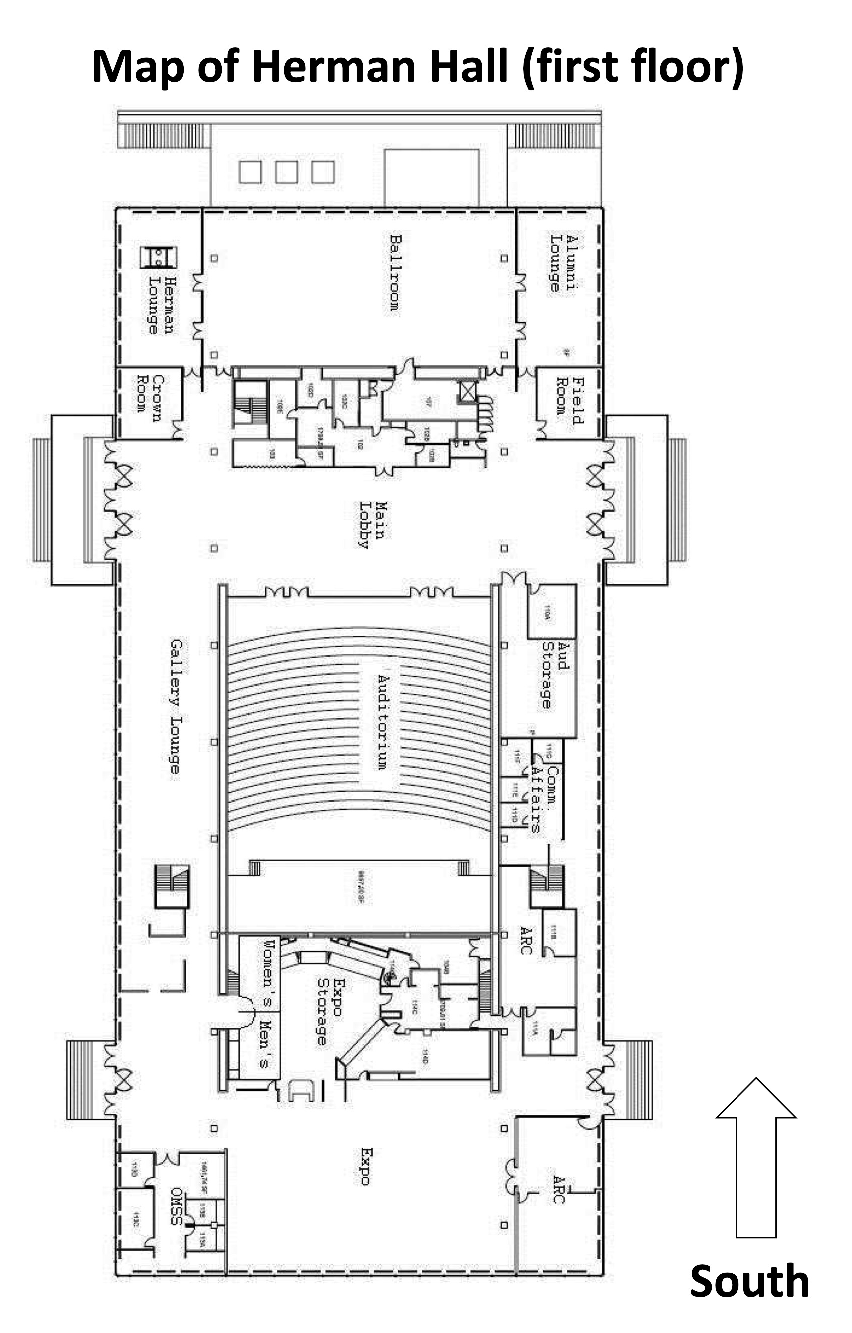
\includegraphics[width =0.95 \textwidth] {Photos/MapHermannHallFirstFloor_cropped.eps}
\end{center}
\clearpage

\section{Getting to Illinois Tech}

\subsection{Local Transportation}
Illinois Tech is located several miles south of downtown.  You  can reach Illinois Tech via 
\begin{itemize}
	\item the Chicago Transit Authority (\href{https://www.transitchicago.com/schedules/}{CTA}) `L' Green or Red Lines, which stop at 35th Street, 
	\item the href{https://www.transitchicago.com/schedules/}{CTA} Route 29 bus, which stops at the corner of State and 32nd Streets, or
	\item taxi, Uber, or Lyft.
	 \item If you are driving to Illinois Tech, there is paid visitor parking in the lot on the east side of State Street between 31st and 32nd Streets (enter via State Street).
\end{itemize}

\subsection{Getting to Chicago}

\begin{itemize}
  \item Two major airports, \href{https://www.flychicago.com/ohare/home/Pages/default.aspx}{O'Hare} and \href{https://www.flychicago.com/midway/pages/default.aspx}{Midway} serve Chicago, and are not far from Illinois Tech.  
  \item Our main domestic passenger rail line is \href{Amtrak}{https://www.amtrak.com/home.html}.
\end{itemize}




\section{Food}

Meals will \emph{not} be provided, except for the Wednesday night conference banquet. There are several places on campus or nearby where you can purchase meals.  They are show in \href{https://www.google.com/maps/d/u/1/edit?mid=1QH5guZDg-m8_f1oO9HgZ5sIL76q1gdk&usp=sharing}{this map}


\arrayrulecolor{black}

\begin{center}
 \begin{longtable}{|| l || l | l | l l||} 
 \hline
 \hline  
  \textbf{JKU Mensa}  & \url{www.mensen.at}  & Mon--Fri & 11:00--13:30  \\ \hline
  1B & \textbf{Cafe Ch@t} & Keplergeb\"{a}ude &  Mon--Thu & 08:00--19:00 \\
     &                    &                         &  Fri & 08:00--14:00 \\ \hline
  1C & \textbf{Science Cafe} & Science Park 3 &  Mon--Thu & 08:00--16:00 \\ 
     &                    &                         &  Fri & 08:00--14:00 \\ \hline
  1D & \textbf{Cafe Sassi} & Bankengeb\"{a}ude &  Mon--Thu & 08:00--16:00 \\
     &                    &  \url{www.sassi.at}  &  Fri & 08:00--14:00 \\ \hline
  1E & \textbf{Teichwerk} & University pond &  Mon--Thu & 08:00--16:00 \\
     &                    & \url{www.dasteichwerk.at}  &  Fri & 08:00--14:00 \\ \hline
  2  & \textbf{KHG Mensa} & Mengerstr. 23 & Mon--Fri & 11:00--13:00  \\ 
  
     &                    & \texttt{https://www.dioezese-linz.at/} & & \\
     &                    &  \texttt{khg/mensa/menueplan}  & & \\ \hline
  3  & \textbf{Winklermarkt} &  Altenbergerstr. 40 & Mon--Thu & 07:30--18:30 \\
     & (Supermarket \& &  \texttt{https://winklermarkt.at/}  & Fri & 07:30--19:00 \\
     & Restaurant) &  \texttt{menuplan/}  & Sat & 07:30--17:00 \\ \hline
  4a  & \textbf{Pizzeria} & Aubrunnerweg 1a & Mon--Sun & 11:00--15:00 \\
     & \textbf{Bella Casa} & Phone: +43-732-245646 &          & 17:00--24:00 \\ \hline
  4b  & \textbf{Chinese Restaurant} & Aubrunnerweg 11 & Mon--Sun & 11:00--14:30 \\
     & \textbf{Jadegarten} & Phone: +43-732-750160 &          & 17:00--23:00 \\ \hline
  5  & \textbf{Restaurant} & Altenbergerstr. 6--8 & Mon--Thu & 10:30--22:00 \\
     & \textbf{Burgerista} &  Phone: +43-50-666666 &  Fri--Sat & 10:30--23:00 \\ 
     &  &                     &  Sun & 10:30--23:00 \\ \hline
  6  & \textbf{Restaurant} & Freist\"{a}dter Str. 297 & Mon--Sat & 11:00--23:00 \\
     & \textbf{Peter's Platz} &  Phone: +43-732-251112                   &  Sun & 11:00--17:00 \\ \hline
  7 & \textbf{Subway} & Freist\"{a}dter Str. 313 & Mon--Sun & 11:00--22:00 \\ \hline
  8  & \textbf{Asian Restaurant} & Freist\"{a}dter Str. 315 & Tue & 11:30--14:30 \\
     & \textbf{Ost18} &  Phone: +43-732-244042              &  Wed--Mon & 11:30--14:30 \\ 
     &  &   &   & 17:30--23:00 \\ \hline
  9  & \textbf{Raab Mensa} & Julius-Raab-Str. 10 & Bar: & \\
     & (Restaurant \& Bar)   & Phone: +43-732-24570 & Mon--Thu & 06:30--23:30\\
     &             & \texttt{www.sommerhaus-hotel.at/} & Sat--Sun & 06:30--11:00 \\
     &                            & \texttt{de/linz\#{}speiseplan} & Restaurant:& \\
     &                            &  & Mon--Sun & 11:30--14:30\\
     &                            &  &  & 17:00--21:00\\ \hline
 10  & \textbf{McDonald's \&} & Freist\"{a}dter Str. 298 & Sun--Thu & 07:00--00:00 \\
     & \textbf{McCafe} &               &  Fri--Sat & 07:00--02:00 \\ \hline
 11  & \textbf{``Penny''} & J.W.-Klein-Str. 58 & Mon--Fri & 07:40--20:00 \\
     & (Supermarket)      &                    & Sat      & 07:40--18:00 \\ \hline 
 12  & \textbf{``Hofer''} & Freist\"{a}dter Str. 401 & Mon--Fri & 07:40--20:00 \\
     & (Supermarket)      &                    & Sat      & 07:40--18:00 \\ \hline 
 13  & \textbf{``Billa''} & Freist\"{a}dter Str. 400 & Mon--Fri & 07:40--20:00 \\
     & (Supermarket)      &                    & Sat      & 07:40--18:00 \\ \hline      
 14  & \textbf{``Spar''} & Altenbergerstr. 69 & Mon--Fri & 07:30--19:45 \\
     & (Supermarket)      &  (on JKU campus)  & Sat      & 08:00--18:00 \\ \hline  
\hline   
\end{longtable}
\end{center}



%\begin{center}
% \includegraphics[width=14cm]{Food_map}
%\end{center}


\section{Technology}

\subsubsection{Equipment in classrooms used for conference}

Each lecture hall is equipped with a desktop computer running Windows,
with USB port access and internet connection, a data projector and screen, 
and blackboards. One MCQMC staff member 
%(with a yellow name tag) 
will be present 
in each lecture hall to assist with IT related issues.

We strongly encourage you to make yourself known to your session chair and (if necessary) 
the MCQMC staff member assigned to your lecture room, prior to your talk. Please prepare your talk in the form of a PDF or PPT document. A slides repository will be created shortly before the conference to facilitate the uploading of slides to the desktop computer in each room prior to each session by MCQMC staff. More detailed instructions will be sent to speakers and session chairs prior to the conference. An alternative option is to bring 
a USB storage device with your slides copied on it and make sure that your talk is copied onto
the desktop computer during the break prior to your talk. 
%We cannot guarantee 
%that other file formats than PDF can be displayed correctly.

If you require access to other software packages or other audio-visual
equipment, please communicate with the conference organizers well ahead of time to
see if it can be arranged. It is possible to connect your personal laptop
to the data projector, but we prefer that you avoid this option due to the
tight conference schedule. If you need to use your own laptop, please make
sure that you discuss this with a MCQMC staff member %assigned to your room 
and 
that you test the connection well before your talk.


\subsubsection{Internet and Computer Access}

University of Waterloo has eduroam to provide free wireless access for visitors whose home
institutions also have eduroam. For more information on eduroam see
\url{http://www.eduroam.org}. Please check with your institution whether you have access to eduroam and
for instructions on how to set up eduroam (this depends on your home
institution and not on local institutions).

If you cannot use eduroam, conference participants will be granted access to the Waterloo wireless network on campus via self-registration. Further details on how to do so will be announced during the opening of the conference. 

%Please note that we are unable to set up new accounts at the conference.

In any case, please use the wireless connections provided responsibly. 

\subsubsection{Power Plugs in Canada}

In Canada, the standard power sockets are:

\begin{itemize}
	\item Type A:
	\begin{itemize}
		\item Description: This socket has two flat parallel pins.
		\item Voltage: 120 V
		\item Frequency: 60 Hz
	\end{itemize}
	
	\item Type B:
	\begin{itemize}
		\item Description: This socket has two flat parallel pins and a grounding pin (three-pronged).
		\item Voltage: 120 V
		\item Frequency: 60 Hz
	\end{itemize}
\end{itemize}

%\begin{center}
%\includegraphics[width=5cm]{Power_Pic}
%\end{center}

\section{Health and Safety}


\subsubsection{Emergency Contacts, Hospitals and Services on Campus}

The emergency phone number in Canada is \textbf{911}. For emergency calls on-campus, call the UW Special Constable at 519-888-4911. There is a Special Constable on campus 24 hours a day, 7 days a week.


\textbf{Local Kitchener-Waterloo Hospitals}

\begin{itemize}
    \item Grand River Hospital, 835 King Street West, Kitchener (519-742-3611)

    \item St. Mary’s General Hospital, 911 Queen’s Boulevard, Kitchener (519-744-3311)
\end{itemize}


\subsubsection{Conference Statistics (as of July 5)}

\begin{center}
 \begin{tabular}{ll}
 Number of participants & 151 \\
 Number of plenary lectures & 8 \\
 Number of tutorials & 2 \\
 Number of talks & 137 \\
 Number of special sessions & 24 (85 talks) \\
 Number of technical sessions & 12 (42 talks) \\
 \end{tabular}
\end{center}  % old

\chapter{List of Participants}

\setlength{\columnsep}{1cm}

\begin{multicols}{2}

\small\raggedright

\participantne{Christiane Lemieux}
{University of Waterloo}
{P2}
{}
\participantne{Peter Glynn}
{Stanford University}
{P3}
{}
\participantne{Roshan Joseph}
{Georgia Institute of Technology}
{P4}
{}
\participantne{Michaela Szölgyenyi}
{University of Klagenfurt}
{P5}
{}
\participantne{Uros Seljak}
{University of California, Berkeley}
{P6}
{}
\participantne{Nicolas Chopin}
{ENSAE, Institut Polytechnique de Paris}
{P7}
{}
\participantne{Veronika Ročková}
{University of Chicago}
{P8}
{}
\participantne{Stefan Heinrich}
{RPTU Kaiserslautern-Landau}
{S1}
{}
\participantne{Thomas Muller-Gronbach}
{University of Passau}
{S1}
{}
\participantne{Andreas Neuenkirch}
{University of Mannheim}
{S1}
{}
\participantne{Christopher Rauhögger}
{University of Passau}
{S1}
{}
\participantne{Verena Schwarz}
{University of Klagenfurt}
{S1}
{}
\participantne{Larisa Yaroslavtseva}
{University of Graz}
{S1}
{}
\participantne{Murat Erdogdu}
{University of Toronto}
{S10}
{}
\participantne{Sebastiano Grazzi}
{Bocconi University}
{S10}
{}
\participantne{Federica Milinanni}
{KTH Royal Institute of Technology}
{S10}
{}
\participantne{Alex Shestopaloff}
{Queen Mary University of London}
{S10}
{}
\participantne{Xingyu Wang}
{University of Amsterdam}
{S10}
{}
\participantne{Jun Yang}
{University of Copenhagen}
{S10}
{}
\participantne{Nikhil Bansal}
{University of Michigan, Ann Arbor}
{S11}
{}
\participantne{Sou-Cheng Choi}
{Illinois Institute of Technology}
{S11}
{}
\participantne{Yuhan Ding}
{Illinois Institute of Technology}
{S11}
{}
\participantne{Hwanwoo Kim}
{Duke University}
{S11}
{}
\participantne{Michael Mascagni}
{Florida State University}
{S11}
{}
\participantne{Jonathan Weare}
{New York University}
{S11}
{}
\participantne{Stefan Heinrich}
{RPTU Kaiserslautern-Landau}
{S12}
{}
\participantne{Fred Hickernell}
{Illinois Institute of Technology}
{S12}
{}
\participantne{Gunther Leobacher}
{University of Graz}
{S12}
{}
\participantne{Thomas Muller-Gronbach}
{University of Passau}
{S12}
{}
\participantne{Alexander Steinicke}
{Technical University of Leoben}
{S12}
{}
\participantne{Larisa Yaroslavtseva}
{University of Graz}
{S12}
{}
\participantne{Alen Alexanderian}
{North Carolina State University}
{S13}
{}
\participantne{Tommie Catanach}
{Sandia National Laboratories}
{S13}
{}
\participantne{Florence Forbes}
{Inria}
{S13}
{}
\participantne{Xun Huan}
{University of Michigan}
{S13}
{}
\participantne{Jacopo Iollo}
{Inria}
{S13}
{}
\participantne{Youssef Marzouk}
{Massachusetts Institute of Technology}
{S13}
{}
\participantne{Eya Ben Amar}
{King Abdullah University of Science and Technology}
{S14}
{}
\participantne{Victor Elvira}
{University of Edinburgh}
{S14}
{}
\participantne{Shyam Mohan Subbiah Pillai}
{RWTH Aachen University}
{S14}
{}
\participantne{Nadhir Ben Rached}
{University of Leeds}
{S14}
{}
\participantne{Shyam Mohan Subbiah Pillai}
{RWTH Aachen University}
{S14}
{}
\participantne{Raúl Tempone}
{King Abdullah University of Science and Technology}
{S14}
{}
\participantne{Bruno Tuffin}
{Inria}
{S14}
{}
\participantne{Sou-Cheng Choi}
{Illinois Institute of Technology}
{S15}
{}
\participantne{Yuhan Ding}
{Illinois Institute of Technology}
{S15}
{}
\participantne{Takashi Goda}
{University of Tokyo}
{S15}
{}
\participantne{Joshua Isaacson}
{Fermilab}
{S15}
{}
\participantne{Ziang Niu}
{University of Pennsylvania}
{S15}
{}
\participantne{Chenyang Zhong}
{Columbia University}
{S15}
{}
\participantne{Stefan Heinrich}
{RPTU Kaiserslautern-Landau}
{S16}
{}
\participantne{Bernd Käßemodel}
{Chemnitz University of Technology}
{S16}
{}
\participantne{Iosif Lytras}
{Athena/archimedes Research Centre, Greece}
{S16}
{}
\participantne{Nikolaos Makras}
{University of Edinburgh}
{S16}
{}
\participantne{Thomas Muller-Gronbach}
{University of Passau}
{S16}
{}
\participantne{Larisa Yaroslavtseva}
{University of Graz}
{S16}
{}
\participantne{Chaofan Huang}
{Georgia Institute of Technology}
{S17}
{}
\participantne{Lulu Kang}
{University of Massachusetts Amherst}
{S17}
{}
\participantne{Chunfang Lin}
{Queen's University}
{S17}
{}
\participantne{Simon Mak}
{Duke University}
{S17}
{}
\participantne{Chih-Li Sung}
{Michigan State University}
{S17}
{}
\participantne{Qian Xiao}
{Shanghai Jiao Tong University}
{S17}
{}
\participantne{Nawaf Bou-Rabee}
{Rutgers University}
{S18}
{}
\participantne{Trevor Campbell}
{University of British Columbia}
{S18}
{}
\participantne{Bob Carpenter}
{Flatiron Institute}
{S18}
{}
\participantne{Chirag Modi}
{New York University}
{S18}
{}
\participantne{Art Owen}
{Stanford University}
{S18}
{}
\participantne{Raghu Bollapragada}
{University of Texas at Austin}
{S19}
{}
\participantne{Shane Henderson}
{Cornell University}
{S19}
{}
\participantne{Raghu Pasupathy}
{Purdue University}
{S19}
{}
\participantne{Jürgen Dölz}
{University of Bonn}
{S2}
{}
\participantne{Philipp Guth}
{Austrian Academy of Sciences}
{S2}
{}
\participantne{Harri Hakula}
{Aalto University}
{S2}
{}
\participantne{Carlos Jerez-Hanckes}
{Universidad Adolfo Ibáñez}
{S2}
{}
\participantne{Vesa Kaarnioja}
{Free University of Berlin}
{S2}
{}
\participantne{André-Alexander Zepernick}
{Free University of Berlin}
{S2}
{}
\participantne{Haotian Jiang}
{University of Chicago}
{S20}
{}
\participantne{Aleksandar Nikolov}
{University of Toronto}
{S20}
{}
\participantne{Peng Zhang}
{Rutgers University}
{S20}
{}
\participantne{Arash Fahim}
{Florida State University}
{S21}
{}
\participantne{Sharanya Jayaraman}
{Florida State University}
{S21}
{}
\participantne{Michael Mascagni}
{Florida State University and National Institute of Standards and Technology}
{S21}
{}
\participantne{Rohan Sawahney}
{Nvidia Corporation}
{S21}
{}
\participantne{Silei Song}
{Florida State University}
{S21}
{}
\participantne{Felix Bartel}
{University of New South Wales}
{S22}
{}
\participantne{Mou Cai}
{University of Tokyo}
{S22}
{}
\participantne{Michael Gnewuch}
{University of Osnabrück}
{S22}
{}
\participantne{Takashi Goda}
{University of Tokyo}
{S22}
{}
\participantne{Zhijian He}
{South China University of Technology}
{S22}
{}
\participantne{Peter Kritzer}
{Austrian Academy of Sciences}
{S22}
{}
\participantne{Frances Y. Kuo}
{University of New South Wales}
{S22}
{}
\participantne{Krishnakumar Balasubramanian}
{University of California, Davis}
{S23}
{}
\participantne{Yifan Chen}
{New York University}
{S23}
{}
\participantne{Xiaoou Cheng}
{New York University}
{S23}
{}
\participantne{Lihan Wang}
{Carnegie Mellon University}
{S23}
{}
\participantne{Jonathan Weare}
{New York University}
{S23}
{}
\participantne{Peter Whalley}
{ETH Zurich}
{S23}
{}
\participantne{Arved Bartuska}
{King Abdullah University of Science and Technology/RWTH Aachen University}
{S24}
{}
\participantne{André Gustavo Carlon}
{RWTH Aachen University}
{S24}
{}
\participantne{Philipp Guth}
{Johann Radon Institute for Computational and Applied Mathematics}
{S24}
{}
\participantne{Matteo Raviola}
{École Polytechnique Fédérale de Lausanne}
{S24}
{}
\participantne{Raúl Tempone}
{King Abdullah University of Science and Technology/RWTH Aachen University}
{S24}
{}
\participantne{Michael Gnewuch}
{University of Osnabrück}
{S25}
{}
\participantne{Takashi Goda}
{University of Tokyo}
{S25}
{}
\participantne{Peter Kritzer}
{Austrian Academy of Sciences}
{S25}
{}
\participantne{Dirk Nuyens}
{KU Leuven}
{S25}
{}
\participantne{Art B. Owen}
{Stanford University}
{S25}
{}
\participantne{Zexin Pan}
{Austrian Academy of Sciences}
{S25}
{}
\participantne{Kosuke Suzuki}
{Yamagata University}
{S25}
{}
\participantne{Yifan Chen}
{New York University}
{S26}
{}
\participantne{Xiaoou Cheng}
{New York University}
{S26}
{}
\participantne{Siddharth Mitra}
{Yale University}
{S26}
{}
\participantne{Molei Tao}
{Georgia Institute of Technology}
{S26}
{}
\participantne{Jonathan Weare}
{New York University}
{S26}
{}
\participantne{Fuzhong Zhou}
{Columbia University}
{S26}
{}
\participantne{Jose Blanchet}
{Stanford University}
{S27}
{}
\participantne{Jing Dong}
{Columbia University}
{S27}
{}
\participantne{Chang-Han Rhee}
{Northwestern University}
{S27}
{}
\participantne{Maksim Chupin}
{King Abdullah University of Science and Technology}
{S28}
{}
\participantne{Zhou Fang}
{Chinese Academy of Sciences}
{S28}
{}
\participantne{Chiheb Ben Hammouda}
{Utrecht University}
{S28}
{}
\participantne{Sophia Münker}
{RWTH Aachen University}
{S28}
{}
\participantne{Muruhan Rathinam}
{University of Maryland, Baltimore}
{S28}
{}
\participantne{Raul Tempone}
{RWTH Aachen University}
{S28}
{}
\participantne{Niklas Baumgarten}
{University of Heidelberg}
{S29}
{}
\participantne{Sou-Cheng Choi}
{Illinois Institute of Technology}
{S29}
{}
\participantne{Joseph Farmer}
{University of Notre Dame}
{S29}
{}
\participantne{Mike Giles}
{University of Oxford}
{S29}
{}
\participantne{Johannes Krotz}
{University of Notre Dame}
{S29}
{}
\participantne{Pieterjan Robbe}
{Sandia National Laboratories}
{S29}
{}
\participantne{Aleksei Sorokin}
{Illinois Institute of Technology}
{S29}
{}
\participantne{Arved Bartuska}
{King Abdullah University of Science and Technology/RWTH Aachen University}
{S3}
{}
\participantne{Truong Vinh Hoang}
{RWTH Aachen University}
{S3}
{}
\participantne{Vesa Kaarnioja}
{Free University of Berlin}
{S3}
{}
\participantne{Sebastian Krumscheid}
{Karlsruhe Institute of Technology}
{S3}
{}
\participantne{Raúl Tempone}
{King Abdullah University of Science and Technology/RWTH Aachen University}
{S3}
{}
\participantne{Sou-Cheng Choi}
{Illinois Institute of Technology}
{S4}
{}
\participantne{Mike Giles}
{University of Oxford}
{S4}
{}
\participantne{Irina-Beatrice Haas}
{University of Oxford}
{S4}
{}
\participantne{Chung Ming Loi}
{Durham University}
{S4}
{}
\participantne{Pieterjan Robbe}
{Sandia National Laboratories}
{S4}
{}
\participantne{Michael Gnewuch}
{Osnabruck University}
{S5}
{}
\participantne{Stefan Heinrich}
{RPTU Kaiserslautern-Landau}
{S5}
{}
\participantne{Larysa Matiukha}
{Illinois Institute of Technology}
{S5}
{}
\participantne{Thomas Muller-Gronbach}
{University of Passau}
{S5}
{}
\participantne{Leszek Plaskota}
{University of Warsaw}
{S5}
{}
\participantne{Kateryna Pozharska}
{Chemnitz University of Technology}
{S5}
{}
\participantne{Larisa Yaroslavtseva}
{University of Graz}
{S5}
{}
\participantne{Arved Bartuska}
{RWTH Aachen University}
{S6}
{}
\participantne{Philipp A. Guth}
{Austrian Academy of Sciences}
{S6}
{}
\participantne{Tapio Helin}
{LUT University}
{S6}
{}
\participantne{Vesa Kaarnioja}
{Free University of Berlin}
{S6}
{}
\participantne{Karina Koval}
{University of Heidelberg}
{S6}
{}
\participantne{Johannes Milz}
{Georgia Institute of Technology}
{S6}
{}
\participantne{Makram Chahine}
{Massachusetts Institute of Technology}
{S7}
{}
\participantne{François Clément}
{University of Washington}
{S7}
{}
\participantne{Nathan Kirk}
{Illinois Institute of Technology}
{S7}
{}
\participantne{Gregory Seljak}
{University of Montréal}
{S7}
{}
\participantne{Jean-Francois Chassagneux}
{ENSAE Paris}
{S8}
{}
\participantne{Goncalo Dos Reis}
{University of Edinburgh}
{S8}
{}
\participantne{Noufel Frikha}
{Paris 1 Pantheon-Sorbonne University}
{S8}
{}
\participantne{Stefan Heinrich}
{RPTU Kaiserslautern-Landau}
{S8}
{}
\participantne{Thomas Muller-Gronbach}
{University of Passau}
{S8}
{}
\participantne{Sotirios Sabanis}
{University of Edinburgh}
{S8}
{}
\participantne{Larisa Yaroslavtseva}
{University of Graz}
{S8}
{}
\participantne{Ayoub Belhadji}
{Massachusetts Institute of Technology}
{S9}
{}
\participantne{Adrien Corenflos}
{University of Warwick}
{S9}
{}
\participantne{Steven Damelin}
{Zbmath Open, European Mathematical Society}
{S9}
{}
\participantne{Florence Forbes}
{Inria}
{S9}
{}
\participantne{Xun Huan}
{University of Michigan}
{S9}
{}
\participantne{Youssef Marzouk}
{Massachusetts Institute of Technology}
{S9}
{}
\participantne{Zhihao Wang}
{University of Copenhagen}
{T1-1}
{}
\participantne{Ruben Seyer}
{Chalmers University of Technology and University of Gothenburg}
{T1-2}
{}
\participantne{Philippe Gagnon}
{Université de Montréal}
{T1-3}
{}
\participantne{Attila Lovas}
{Hun-Ren Alfréd Rényi Institute of Mathematics}
{T10-1}
{}
\participantne{Sara Pérez-Vieites}
{Aalto University}
{T10-2}
{}
\participantne{Fabio Zoccolan}
{EPFL}
{T11-1}
{}
\participantne{Adrien Richou}
{Université de Bordeaux}
{T11-2}
{}
\participantne{Anke Wiese}
{Heriot-Watt University}
{T11-3}
{}
\participantne{Riccardo Saporiti}
{EPFL}
{T11-4}
{}
\participantne{Abdujabar Rasulov}
{University of World Economy and Diplomacy}
{T12-1}
{}
\participantne{Miguel Alvarez}
{King Abdullah University of Science and Technology}
{T12-2}
{}
\participantne{Håkon Hoel}
{University of Oslo}
{T12-3}
{}
\participantne{Noufel Frikha}
{Université Paris 1 Panthéon Sorbonne}
{T12-4}
{}
\participantne{Frédéric Blondeel}
{Kuleuven and Unife}
{T13-1}
{}
\participantne{Du Ouyang}
{Tsinghua University}
{T13-2}
{}
\participantne{Wei Cai}
{Southern Methodist University}
{T13-3}
{}
\participantne{Yiqing Zhou}
{KU Leuven}
{T13-4}
{}
\participantne{Reuben Cohn-Gordon}
{University of California, Berkeley}
{T14-1}
{}
\participantne{Philip Schaer}
{Friedrich Schiller University Jena}
{T14-2}
{}
\participantne{Annabelle Carrell}
{University of Cambridge}
{T14-3}
{}
\participantne{Philippe Blondeel}
{Belgian Military Academy}
{T15-1}
{}
\participantne{Rino Persiani}
{INFN Catania}
{T15-2}
{}
\participantne{Prasanth Shyamsundar}
{Fermi National Accelerator Laboratory}
{T15-3}
{}
\participantne{Nicole Aretz}
{University of Texas at Austin}
{T15-4}
{}
\participantne{Kazeem Adeleke}
{University of the West of England}
{T16-1}
{}
\participantne{Carles Domingo-Enrich}
{Microsoft Research New England}
{T16-2}
{}
\participantne{Christopher Draper}
{Florida State University}
{T16-3}
{}
\participantne{Yiming Xu}
{University of Kentucky}
{T16-4}
{}
\participantne{Lorenzo Nagar}
{Basque Center for Applied Mathematics}
{T2-1}
{}
\participantne{Hamza Ruzayqat}
{King Abdullah University of Science and Technology}
{T2-2}
{}
\participantne{Arghya Datta}
{Université de Montréal}
{T2-3}
{}
\participantne{Jimmy Lederman}
{University of Chicago}
{T2-4}
{}
\participantne{Yashveer Kumar}
{INESC-ID}
{T3-1}
{}
\participantne{Serena Fattori}
{Istituto Nazionale di Fisica Nucleare (INFN)}
{T3-2}
{}
\participantne{Muhammad Noor ul Amin}
{COMSATS University Islamabad, Lahore}
{T3-3}
{}
\participantne{Chi-Ok Hwang}
{Gwangju Institute of Science and Technology}
{T3-4}
{}
\participantne{Christian Weiss}
{Ruhr West University of Applied Sciences}
{T4-1}
{}
\participantne{Sifan Liu}
{Flatiron Institute}
{T4-2}
{}
\participantne{Ambrose Emmett-Iwaniw}
{University of Waterloo}
{T4-3}
{}
\participantne{Claude Hall}
{Illinois Institute of Technology}
{T4-4}
{}
\participantne{Peter Kritzer}
{Austrian Academy of Sciences}
{T5-1}
{}
\participantne{Yang Liu}
{King Abdullah University of Science and Technology}
{T5-2}
{}
\participantne{Jakob Dilen}
{KU Leuven}
{T5-3}
{}
\participantne{Aadit Jain}
{Rancho Bernardo High School}
{T5-4}
{}
\participantne{Akash Sharma}
{Chalmers Institute of Technology}
{T6-1}
{}
\participantne{Joonha Park}
{University of Kansas}
{T6-2}
{}
\participantne{Arne Bouillon}
{KU Leuven}
{T6-3}
{}
\participantne{Alex Shkolnik}
{University of California, Santa Barbara}
{T6-4}
{}
\participantne{Kun-Lin Kuo}
{National University of Kaohsiung}
{T7-1}
{}
\participantne{Sascha Holl}
{Max Planck Institute for Informatics}
{T7-2}
{}
\participantne{Josephine Westermann}
{Heidelberg University}
{T7-3}
{}
\participantne{Soumyadip Ghosh}
{IBM Research}
{T7-4}
{}
\participantne{Matyokub Bakoev}
{MGIMO, Tashkent}
{T8-1}
{}
\participantne{Leon Wilkosz}
{King Abdullah University of Science and Technology}
{T8-2}
{}
\participantne{Vincent Zhang}
{University of Southern California}
{T8-3}
{}
\participantne{Hao Quan}
{University of Waterloo}
{T8-4}
{}
\participantne{Nicola Branchini}
{University of Edinburgh}
{T9-1}
{}
\participantne{Daniel Yukimura}
{Impa, Rio de Janeiro}
{T9-2}
{}
\participantne{Toon Ingelaere}
{KU Leuven}
{T9-3}
{}
\participantne{Amit Subrahmanya}
{Virginia Tech}
{T9-4}
{}
\participantne{Hongmei Chi}
{Florida Aandm University}
{}
{}
\participantne{Toni Karvonen}
{LUT University}
{}
{}
\end{multicols}

 % generated by MakeListPart.py

\end{document}